\chapter{Calibration Hardware for Single-Phase}
\label{ch:sp-calib}

%%%%%%%%%%%%%%%%%%%%%%%%%%%%%%%%%%%%%%%%%%%%%%%%%%%%%%%
\section{Calibration Hardware Overview}
\label{sec:sp-calib-ov}

%\section{Calibration Hardware Overview}
%\label{sec:sp-calib-ov}


%%%%%%%%%%%%%%%%%%%%%%%%%%%%
%\fixme{SG:A paragraph length preamble 0 goes before Introduction as suggested by Tim; SG to edit in}

%\subsection{DUNE Calibration Strategy}
\label{sec:sp-calib-ov-intro}

%\fixme{(from Nora) I must point out that the headings in this document are problematic. They go to five levels, in some places (see page 7 on the PDF) with no text until the fifth level heading. This is extremely troubling. Generally, no heading should appear without at least transitional text following it, and here we have three headings with nothing, no content, no transitions, no indications of anything. This will not do. This is especially troublesome later in the chapter when bold is used to designate sections without using headings at all (see page 8 of the PDF). I strongly advise cutting the levels of heading down to three and making sure that text follows each heading. Major headings could use introductory text for that section/chapter while most subheadings should have content following. If you look, you will note that you already have text that can be used for those purposes. For instance, Section 1.1.1 is an introduction to the entire chapter. Some portions of this introduction appear to go with Section 1.1, the overview of the first part. One way to handle this is to put all the headings into a separate file and find the information that goes with the headings. You can then copy and paste the text to the appropriate section with the appropriate heading. If the heading has no text, that heading would be eliminated or text would be provided. This gives you a visual of how the paper fits together. One final note: too many headings cause confusion. (Too few headings also cause confusion.)}

A detailed understanding of the overall detector response is essential for achieving \dword{dune} physics goals. The precision with which each calibration parameter must be measured is spanned by the requirements on the %JM
systematic uncertainties for the \dword{lbl} %, low-energy (\dword{snb}), and other 
and \dword{snb} physics programs at \dword{dune}. The calibration 
program 
%plan %JM;
must generally provide measurements at the few-percent-or-better 
%few-percent %JM; SG: this was a language edit from editors
level stably across an enormous volume and over a long period and provide sufficient redundancy. The Physics volume of the \dword{tdr} provides a detailed description of the calibration strategy for the \dword{dune} \dword{fd}; here, we provide a brief summary.

The current calibration strategy for \dword{dune} uses existing sources of particles, external measurements, and dedicated external calibration hardware systems. Existing calibration sources for \dword{dune} include beam or atmospheric neutrino-induced samples, cosmic rays, argon isotopes, and instrumentation devices such as \dword{lar} purity and temperature monitors. Dedicated calibration hardware systems consist of laser  and neutron source deployment systems.  External measurements by \dword{protodune} and \dword{sbn} experiments  will validate techniques, tools, and the design of systems applicable to the \dword{dune} calibration program. These sources and systems provide measurements of the detector response model parameters, or provide tests of the response model itself. Calibration measurements can also provide corrections to data, data-driven efficiencies, systematics, and particle responses.

%Chapter~4 of the Physics volume of the \dword{tdr} provides a more detailed description of the calibration strategy for the \dword{dune} \dword{fd}. 
%using existing sources of particles (e.g., cosmic ray muons), external measurements (e.g., \dword{protodune}), monitors (e.g., purity monitors), and dedicated calibration hardware systems. 

This chapter focuses on describing the dedicated calibration hardware systems to be deployed for the \dword{dune} \dword{spmod} that provide necessary information beyond the reach of external measurements and existing sources and monitors. These include an ionization laser system, a \phel laser system, and a \dlong{pns} system. The possibility of deploying a radioactive source system is also currently being explored. The responsibility of the calibration hardware systems falls under the joint \dword{sp} and \dword{dp} calibration consortium, which was formed in November 2018.

%This chapter describes the design of the dedicated calibration systems to be deployed for the DUNE \spmod.  As discussed in the Physics TDR\fixme{proper reference}, the calibration strategy includes external measurements (e.g. ProtoDUNE), monitors (e.g. purity, thermal), existing sources of particles (e.g. muons from cosmic rays), and dedicated external calibration hardware systems.  This chapter discusses the calibration hardware systems. Monitoring systems are discussed in other chapters: CISC (purity, thermal monitors, slow control), PDS (LED stability system\fixme{proper name is?}), and CE (charge injection system). The physics TDR discusses the use of existing sources of particles, and external measurements. 

Once the far detector is filled and at the desired high voltage, it immediately becomes live for \dword{snb} and proton decay signals (beam and atmospheric neutrino physics will require a few years of data accumulation), at which point %it is critical for %for %JM
early calibration must track %to track %JM
the space-time dependence of the detector. Dedicated early calibration runs using calibration hardware systems will develop and tune calibration tools to beam data taking and correct for any space-time irregularities observed in the \dword{tpc}. Given the expected low rate of cosmic ray events at the underground location, calibration with cosmic rays is not possible over short time scales and will proceed from coarse-grained to fine-grained over the course of years, as statistics accumulate. 
The experiment will rely on calibration hardware systems, such as a laser system, for calibrations that require an independent probe with reduced or removed interdependencies, fine-grained measurements (both in space and time), and detector stability monitoring on the time scales required by physics. The neutron source system will provide low-energy electromagnetic response at the precision required for low-energy \dword{snb} physics. 
Once the detector is running stably, dedicated calibration runs, ideally before, during, and after each run period, will ensure that detector conditions have not significantly changed. As \dword{dune} becomes systematics-limited, dedicated precision-calibration campaigns using the calibration hardware systems will become crucial for meeting the stringent physics requirements on energy scale reconstruction and detector resolution.

%Section~\ref{sec:sp-calib-ov-scope} describes the baseline calibration hardware designs. 
%and outlines alternative designs that may improve the physics capability and/or reduce overall cost. 
Section~\ref{sec:sp-calib-ov} describes the baseline calibration hardware designs. Section~\ref{sec:sp-calib-sys-las-ion} describes the baseline design for the ionization laser system that provides an independent, fine-grained measurement of the electric field throughout the detector, which is an essential parameter that affects the spatial and energy resolution of physics signals. 
Volume~\volnumberphysics, \voltitlephysics of this \dword{tdr}
%The DUNE \dword{cdr}~\cite{Acciarri:2015uup} 
assumes that the \dword{fv} is known to the \SI{1}{\%} level. Through measurements of the spatial distortions and drift velocity map, the laser calibration system mainly helps define the detector \dword{fv}, thus allowing for the correct prediction of the \dword{fd} spectra. The laser system also offers many secondary uses such as alignment checks, stability monitoring, and diagnosing detector performance issues. Alternative designs for the ionization laser system that may improve the physics capability and/or reduce overall cost are also under development and are described in Appendix~\ref{sec:lasertopfcpen}. %{sec:sp-calib-laser-alter}.
Section~\ref{sec:sp-calib-sys-las-pe} describes the \phel laser system that can be used to rapidly diagnose electronics or \dword{tpc} response issues along with many other useful measurements such as integrated field across drift, drift velocity, and electronics gain. 

Section~\ref{sec:sp-calib-sys-pns} describes the baseline design for the \dword{pns} system, which provides a triggered, well defined, energy deposition from neutron capture in Ar detectable throughout the detector volume. Neutron capture is an important component of signal processes for \dword{snb} and \dword{lbl} physics, enabling direct testing of the detector response spatially and temporally for the low-energy program and the efficiency of the detector in reconstructing the low-energy spectra. The proposed \dword{rsds}, 
%radioactive source system
which is in many ways complementary to the \dword{pns}
%pulsed neutron source 
system, can provide at known locations inside the detector a source of gamma rays in the same energy range of \dword{snb} and solar neutrino physics. But the \dword{rsds} is the only calibration system that could probe the detection capability for single isolated solar neutrino events and study how well radiological backgrounds can be suppressed. In contrast, the \dword{pns} is externally triggered and does not provide such a well defined source location for gamma rays inside the detector. On the other hand, the \dword{pns} can probe the uniformity of the full detector, while the \dword{rsds} could only scan the ends of the detector. A possible  complementary \dword{rsds} system is described in the Appendix~\ref{sec:sp-calib-sys-rsds}. 

The \dword{daq} requirements for calibration systems are described in Section~\ref{sec:sp-calib-daqreq}. For all the calibration hardware systems, the goal is to deploy prototype designs and validate them at \dword{protodune} during the post long shutdown 2 (LS2) running  at \dword{cern}. The validation plan for calibration systems at \dword{protodune} and other experiments is described in Section~\ref{sec:sp-calib-val}. 
The schedule and milestones for calibration systems is discussed in Section~\ref{sec:sp-calib-sched}.

%The calibration consortium was formed in November 2018. Significant development plans exist, and their timeline is in Section~\ref{sec:sp-calib-sched}.
%A large part of the work done so far has been done within the Calibration Task Force; 

%%%%%%%%%%%%%%%%%%%%%%%%%%%%
\subsection{Scope}
\label{sec:sp-calib-ov-scope}
% KM outline
%% Scope is: baseline designs for Laser system and neutron system.
%% Alternative designs, including additional capabilities of the laser system, radioactive source are considered.

%%calibration review in May. "what's the scope? How many lasers we need? How many ports needed? Do we need crossing tracks? do we need to penetrate FC ? what does the HV consortium think about that?"

The scope of the calibration consortium includes a laser ionization system, a \phel laser system, a laser positioning system, and a \dlong{pns}
%pulsed neutron source 
system. In addition, the consortium is evaluating a \dlong{rsds}.
%radioactive source system
 The calibration consortium is responsible for design through commissioning in the \dword{sp} module for these calibration devices and their associated feedthroughs. Validating the designs of calibration systems at \dword{protodune} (and other experiments as relevant) is also included under the scope of the consortium. Figure~\ref{fig:calib_scope_chart} shows the subsystems included under the calibration consortium. 

Chapters 3, 4, 5, and 8 \fixme{add refs} describe other hardware essential for calibration such as \dword{ce} external charge injection systems, \dword{hv} monitoring devices, \dword{pds},
stability monitoring system, and cryogenic instrumentation and detector monitoring devices. The scope of these systems is described by their respective consortia, and the calibration consortium has substantial interfaces with these consortia. 

The use of other calibration sources such as external measurements and existing sources of particles (e.g., muons, pions) is discussed in the physics volume of the \dword{tdr}. The calibration task force is pursuing the effects of calibration on physics and related studies, and the consortium works closely with the task force to make physics connections. Calibrations also require simulations (e.g. \efield) to identify desirable locations for calibration devices in the cryostat, away from regions of high \efield, so that their presence does not induce large field distortions. 
%Calibration has additional activities outside the scope of the consortium that require coordination with other groups. This is discussed in Section~\ref{sec:sp-calib-intfc}. 
The design of the calibration systems and understanding the related physics requires coordination with other consortia and groups. This is discussed in Section~\ref{sec:sp-calib-intfc}.
%, which also includes necessary tools (e.g., physics simulations) developed in conjunction with the physics groups and calibration task force.

%\fixme{Please use dunefigures! Here's a template (the label should be fig:filename):}

%\begin{dunefigure}[short caption]{label}
%{long caption}
%\includegraphics[width=0.8\textwidth]{filename}
%\end{dunefigure}

%\begin{figure}[tbp]
%\centering
%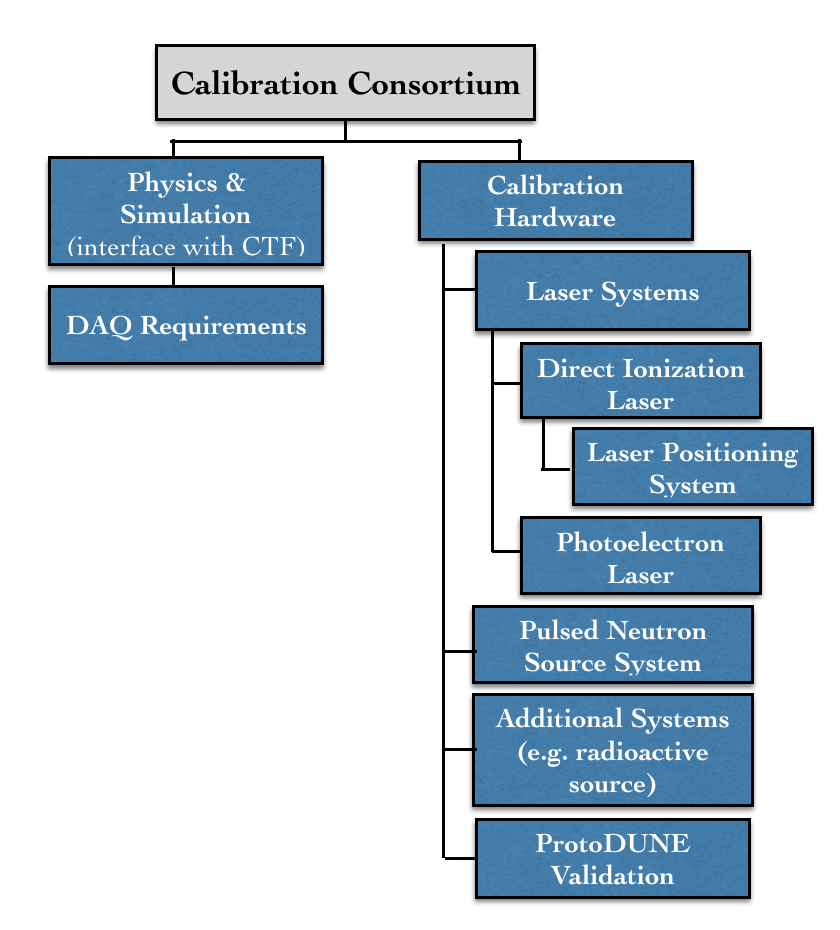
\includegraphics[height=4.0in]{graphics/calib_scope_chart.png}
%\caption{Calibration consortium subsystem chart.}
%\label{fig:scope_chart}
%\end{figure}

\begin{dunefigure}[Calibration consortium subsystem chart]{fig:calib_scope_chart}
{Calibration consortium subsystem chart.}
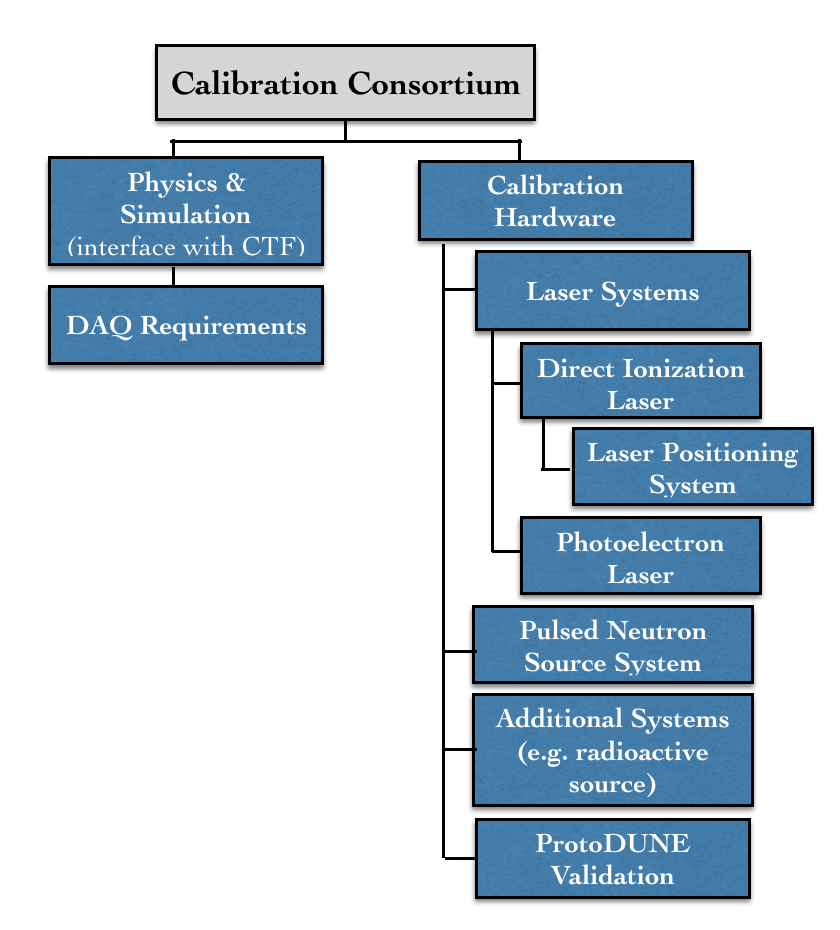
\includegraphics[height=4.0in]{graphics/calib_scope_chart.png}
\end{dunefigure}

%%%%%%%%%%%%%%%%%%%%%%%%%%%%
%\subsection{Requirements}
%\label{sec:sp-calib-ov-req}

%\input{vol-sp/ch-sp-calib-requirements}


%%%%%%%%%%%%%%%%%%%%%%%%%%%%
\subsection{Design Considerations and Requirements}
\label{sec:sp-calib-ov-consid}
%\fixme{SG, KM: Done; JM please check. }
%To-DO: Need more information on requirements from neutron source and RA source, once we have it, we can update the text/table as needed.}

Some common design considerations for calibration devices include stability, reliability, and longevity, so calibration systems can be operated for the lifetime of the experiment (\dunelifetime). Such longevity is uncommon for any device, so the overall design permits replacing devices where possible. The systems must also adhere to relevant global requirements of the \dword{dune} detector. Table~\ref{tab:specs:SP-CALIB} shows the top-level overall requirements for calibration subsystems. For example, \dword{dune} requires the \efield  on any instrumentation devices inside the cryostat to be less than 30 kV/cm to minimize the risk of dielectric breakdown in \dword{lar}. Another consideration important for reconstructing events is the maximum noise level the readout electronics can tolerate from calibration devices. \dword{pdsp} is evaluating this. 

 For the laser system, the energy and position reconstruction requirements for physics measurements lead to requirements for the necessary precision in measuring the laser \efield as well as its spatial coverage and granularity. The laser \efield measurement precision must be about \SI{1}{\%} so that the effect on the collected charge is well below \SI{1}{\%}. This is also motivated by consistency with the high level \dword{dune} specification of \SI{1}{\%} on field uniformity throughout the volume for component alignment and the \dword{hv} system. For laser coverage, to keep the \efield measurement at the $\sim$\SI{1}{\%} level, we are aiming for a coverage of \SI{75}{\%} or more of the total \dword{fv}. The requirement on granularity for the laser is estimated based on the \dword{fv} uncertainty requirements (\SI{1}{\%}) and corresponding uncertainty requirements (\SI{1.5}{\cm}) in each coordinate. A voxel size of \num{30}$\times$\num{30}$\times$\SI{30}{\cubic\cm} should be sufficient to satisfy the \dword{fv} uncertainty requirements. 

The laser beam position must also meet the level of reconstruction requirement in each coordinate, approximately \SI{5}{\milli\m} over \num{5} to \SI{10}{\m}, where the latter is the distance between two consecutive laser ports in the beam direction. This results in a stringent requirement of \ang{0.03} (or \SI{0.5}{\mrad}). The data volume for the ionization laser system must be at least \num{90}~TB/year/\SI{10}{\kt}, assuming \num{800}k laser pulses, \num{10}$\times$\num{10}$\times$\SI{10}{\cubic\cm} voxel sizes, a \SI{100}{\micro\s} zero suppression window, and one dedicated calibration campaign per year.

For the \dword{pns} system, the system must provide a sufficient neutron event rate to make spatially separated precision measurements across the detector of a comparable size to the voxels probed by the laser (\num{30}$\times$\num{30}$\times$\SI{30}{\cubic\cm}) for most regions of the detector (\SI{75}{\%}). 
% 1st draft
%For the supernova program, measurements from the \dword{pns} \fixme{This abbreviation is in neither glossary.} should demonstrate 1\% energy scale, 5\% energy resolution, and 0.5 MeV detection threshold, so each voxel should have sufficient neutron event rate to achieve this. %\todo{KM: Improve or remind connection to SN program? even though it's comparable? SG: maybe for 2nd draft?}
%rewritten for 2nd draft
For the \dword{snb} program, the sensitivity to distortions of the neutrino energy spectrum depends on the uncertainties in the detection threshold and the reconstructed energy scale and resolution. Studies discussed in the physics \dword{tdr} present target ranges for the uncertainties in these parameters as a function of energy. The measurements with the \dword{pns} aim to provide response corrections and performance estimates, so those uncertainty targets are met throughout the whole volume, and so each voxel has a sufficient neutron event rate (percent level statistical uncertainty).

%\fixme{Insert correct reference to physics TDR ch7}
%\fixme{Put PNS in glossary and use that.}


In terms of data volume requirements, the \dword{pns} system requires about \num{84}~TB/year/\SI{10}{\kt} assuming \num{e6} neutrons/pulse, \num{1000} neutron captures/\si{\cubic\m},
%m$^{3}$ 
and \num{1300} observed neutron captures per pulse, and six calibration runs per year. 



Table~\ref{tab:fdgen-calib-all-reqs} shows the full set of requirements related to all calibration subsystems. More details on each of the requirements can be found under corresponding consortia.   
\todo{SP-CALIB-3 is coming out weird in table 1.1, needs to be fixed.}

%\fixme{Can the second part of this title be put in a footnote to Table 1.1? SG: we would prefer to leave it here}


%% This file is generated, any edits may be lost.

\begin{longtable}{p{0.14\textwidth}p{0.13\textwidth}p{0.18\textwidth}p{0.22\textwidth}p{0.20\textwidth}}
\caption{Specifications for SP-CALIB \fixmehl{ref \texttt{tab:spec:SP-CALIB}}} \\
  \rowcolor{dunesky}
       Label & Description  & Specification \newline (Goal) & Rationale & Validation \\  \colhline

   \newtag{SP-CALIB-1}{ spec:efield-calib-precision }  & Ionization laser electric field measurement precision  &  \SI{1}{\%} \newline ( $<$\SI{1}{\%} ) &  Electric field affects energy and position measurements. &  ProtoDUNE and external experiments. \\ \colhline
     % 1
   \newtag{SP-CALIB-2}{ spec:efield-calib-coverage }  & Ionization laser \efield measurement coverage  &  $>\,\SI{75}{\%}$ \newline ( \SI{100}{\%} ) &  Allowable size of the uncovered detector regions is set by the highest reasonably expected field distortions, 4%. &  ProtoDUNE \\ \colhline
     % 2
   \newtag{SP-CALIB-3}{ spec:efield-calib-granularity }  & Ionization laser \efield measurement  granularity  &  $<\,\SI{30\times30\times30}{\centi\meter}$ \newline ( $<\,\SI{10\times10\times10}{\centi\meter}$ ) &  Minimum measurable region is set by the maximum expected distortion and position reconstruction requirements. &  ProtoDUNE \\ \colhline
     % 3
   \newtag{SP-CALIB-4}{ spec:laser-position-precision }  & Laser beam position precision  &  $~\SI{0.5}{\milli\radian}$ \newline ($<\SI{0.5}{\milli\radian}$) &  The necessary spatial precision does not need to be smaller than the APA wire gap. &  ProtoDUNE \\ \colhline
     % 4
   \newtag{SP-CALIB-5}{ spec:neutron-source-coverage }  & Neutron source coverage  &  $>$\SI{75}{\%} \newline ( \SI{100}{\%} ) &  The coverage of the pulsed neutron system depends on the energy resolution requirements at low energy. &  Simulations \\ \colhline
     % 5
   \newtag{SP-CALIB-6}{ spec:data-volume-laser }  & Ionization laser data volume per year (per 10 kt)  &  $>\SI{184}{TB/yr/10 kt}$ \newline ($>\SI{368}{TB/yr/10 kt}$) &  The laser data volume must allow the needed coverage and granularity. &  ProtoDUNE and simulations \\ \colhline
     % 6
   \newtag{SP-CALIB-7}{ spec:data-volume-pns }  & Neutron source DAQ rate per year (per 10 kton)  &  $>$\SI{84}{TB/yr/10 kton} \newline ( $>$\SI{168}{TB/yr/10 kton} ) &  The coverage of the pulsed neutron system depends on the energy resolution requirements at low energy. &  Simulations \\ \colhline
     % 7


\label{tab:specs:just:SP-CALIB}
\end{longtable}

% This file is generated, any edits may be lost.

\begin{longtable}{p{0.14\textwidth}p{0.13\textwidth}p{0.18\textwidth}p{0.22\textwidth}p{0.20\textwidth}}
\caption{Specifications for SP-CALIB \fixmehl{ref \texttt{tab:spec:SP-CALIB}}} \\
  \rowcolor{dunesky}
       Label & Description  & Specification \newline (Goal) & Rationale & Validation \\  \colhline

   \newtag{SP-FD-1}{ spec:min-drift-field }  & Minimum drift field  &  $>$\,\SI{250}{ V/cm} \newline ( $>\,\SI{500}{ V/cm}$ ) &  Lessens impacts of $e^-$-Ar recombination, $e^-$ lifetime, $e^-$ diffusion and space charge. &  ProtoDUNE \\ \colhline
    
   
  \newtag{SP-FD-2}{ spec:system-noise }  & System noise  &  $<\,\SI{1000}\,e^-$ &  Provides $>$5:1 S/N on induction planes for  pattern recognition and two-track separation. &  ProtoDUNE and simulation \\ \colhline
    
   
  \newtag{SP-FD-3}{ spec:light-yield }  & Light yield  &  $>\,\SI{20}{PE/MeV}$ (avg), $>\,\SI{0.5}{PE/MeV}$ (min) &  Gives PDS energy resolution comparable that of the TPC for 5-7 MeV SN $\nu$s, and allows tagging of $>\,\SI{99}{\%}$ of nucleon decay backgrounds with light at all points in detector. &  Supernova and nucleon decay events in the FD with full simulation and reconstruction. \\ \colhline
    
    \\ \rowcolor{dunesky} \newtag{SP-FD-4}{ spec:time-resolution-pds } & Name: Time resolution \\
    Description & The time resolution of the photon detection system shall be less than 1 microsecond in order to assign a unique event time.   \\  \colhline
    Specification (Goal) &  $<\,\SI{1}{\micro\second}$  ( $<\,\SI{100}{\nano\second}$ ) \\   \colhline
    Rationale &   Enables \SI{1}{mm} position resolution for \SI{10}{MeV} SNB candidate events for instantaneous rate $<\,\SI{1}{m^{-3}ms^{-1}}$.  \\ \colhline
    Validation &   \\
   \colhline

   \newtag{SP-FD-5}{ spec:lar-purity }  & Liquid argon purity  &  $<$\,\SI{100}{ppt} \newline ($<\,\SI{30}{ppt}$) &  Provides $>$5:1 S/N on induction planes for  pattern recognition and two-track separation. &  Purity monitors and cosmic ray tracks \\ \colhline
    
    \\ \rowcolor{dunesky} \newtag{SP-FD-7}{ spec:misalignment-field-uniformity } & Name: Drift field uniformity due to component alignment \\
    Description & Misalignments of the various TPC components shall not introduce drift-field nonuniformities beyond those specified in the HVS requirements.   \\  \colhline
    Specification &  $<\,1\,$\% throughout volume \\   \colhline
    Rationale &   Maintains APA, CPA,  FC orientation and shape.  \\ \colhline
    Validation & ProtoDUNE  \\
   \colhline

    
   
  \newtag{SP-FD-9}{ spec:apa-wire-spacing }  & APA wire spacing  &  \SI{4.669}{mm} for U,V; \SI{4.790}{mm} for X,G &  Enables 100\% efficient MIP detection, \SI{1.5}{cm} $yz$ vertex resolution. &  Simulation \\ \colhline
    
    \\ \rowcolor{dunesky} \newtag{SP-FD-11}{ spec:hvs-field-uniformity } & Name: Drift field uniformity due to HVS \\
    Description & Design of TPC cathode and FC components shall ensure uniform field.  Production tolerances shall be set so as to maintain flatness of component surfaces and, by extension, the shape of the drift field volume.   \\  \colhline
    Specification &  $<\,\SI{1}{\%}$ throughout volume \\   \colhline
    Rationale &   High reconstruction efficiency.  \\ \colhline
    Validation & ProtoDUNE and simulation  \\
   \colhline

    
   \newtag{SP-FD-13}{ spec:fe-peak-time }  & Front-end peaking time  &  \SI{1}{\micro\second} \newline ( Adjustable so as to see saturation in less than \SI{10}{\%} of beam-produced events ) &  Vertex resolution; optimized for \SI{5}{mm} wire spacing. &  ProtoDUNE and simulation \\ \colhline
    
   
  \newtag{SP-FD-16}{ spec:det-dead-time }  & Detector dead time  &  $<\,\SI{0.5}{\%}$ &  Meet physics goals in timely fashion. &  ProtoDUNE \\ \colhline
    
   
  \newtag{SP-FD-22}{ spec:data-rate-to-tape }  & Data rate to tape  &  $<\,\SI{30}{PB/year}$ &  Cost.  Bandwidth. &  ProtoDUNE \\ \colhline
    
   
  \newtag{SP-FD-23}{ spec:sn-trigger }  & Supernova trigger  &  $>\,\SI{90}{\%}$ efficiency for SNB within \SI{100}{kpc} &  $>\,$90\% efficiency for SNB within 100 kpc &  Simulation and bench tests \\ \colhline
    
    \\ \rowcolor{dunesky} \newtag{SP-FD-24}{ spec:local-e-fields } & Name: Local electric fields \\
    Description & The integrated detector design shall minimize potential pathways for HV discharges.   \\  \colhline
    Specification &  $<\,\SI{30}{kV/cm}$ \\   \colhline
    Rationale &   Maximize live time; maintain high S/N.  \\ \colhline
    Validation & ProtoDUNE  \\
   \colhline

   
  \newtag{SP-FD-25}{ spec:non-fe-noise }  & Non-FE noise contributions  &  $<<\,\SI{1000}{enc} $ &  High S/N for high reconstruction efficiency. &  Engineering calculation and ProtoDUNE \\ \colhline
    
    \\ \rowcolor{dunesky} \newtag{SP-FD-26}{ spec:lar-impurity-contrib } & Name: LAr impurity contributions from components \\
    Description & Contributions to LAr contamination from detector components, through outgassing or other processes, shall remain << 30 ppt so as to avoid significantly increasing the nominal level of contamination.   \\  \colhline
    Specification &  $<<\,\SI{30}{ppt} $ \\   \colhline
    Rationale &   Maintain HV operating range for high live time fraction.  \\ \colhline
    Validation & ProtoDUNE  \\
   \colhline

    \\ \rowcolor{dunesky} \newtag{SP-FD-27}{ spec:radiopurity } & Name: Introduced radioactivity \\
    Description & Introduced radioactivity shall be less than that from 39Ar.   \\  \colhline
    Specification &  less than that from $^{39}$Ar \\   \colhline
    Rationale &   Maintain low radiological backgrounds for SNB searches.  \\ \colhline
    Validation & ProtoDUNE and assays during construction  \\
   \colhline


   \newtag{SP-CALIB-1}{ spec:efield-calib-precision }  & Ionization laser electric field measurement precision  &  \SI{1}{\%} \newline ( $<$\SI{1}{\%} ) &  Electric field affects energy and position measurements. &  ProtoDUNE and external experiments. \\ \colhline
    
   \newtag{SP-CALIB-2}{ spec:efield-calib-coverage }  & Ionization laser \efield measurement coverage  &  $>\,\SI{75}{\%}$ \newline ( \SI{100}{\%} ) &  Allowable size of the uncovered detector regions is set by the highest reasonably expected field distortions, 4%. &  ProtoDUNE \\ \colhline
    
   \newtag{SP-CALIB-3}{ spec:efield-calib-granularity }  & Ionization laser \efield measurement  granularity  &  $<\,\SI{30\times30\times30}{\centi\meter}$ \newline ( $<\,\SI{10\times10\times10}{\centi\meter}$ ) &  Minimum measurable region is set by the maximum expected distortion and position reconstruction requirements. &  ProtoDUNE \\ \colhline
    
   \newtag{SP-CALIB-4}{ spec:laser-position-precision }  & Laser beam position precision  &  $~\SI{0.5}{\milli\radian}$ \newline ($<\SI{0.5}{\milli\radian}$) &  The necessary spatial precision does not need to be smaller than the APA wire gap. &  ProtoDUNE \\ \colhline
    
   \newtag{SP-CALIB-5}{ spec:neutron-source-coverage }  & Neutron source coverage  &  $>$\SI{75}{\%} \newline ( \SI{100}{\%} ) &  The coverage of the pulsed neutron system depends on the energy resolution requirements at low energy. &  Simulations \\ \colhline
    
   \newtag{SP-CALIB-6}{ spec:data-volume-laser }  & Ionization laser data volume per year (per 10 kt)  &  $>\SI{184}{TB/yr/10 kt}$ \newline ($>\SI{368}{TB/yr/10 kt}$) &  The laser data volume must allow the needed coverage and granularity. &  ProtoDUNE and simulations \\ \colhline
    
   \newtag{SP-CALIB-7}{ spec:data-volume-pns }  & Neutron source DAQ rate per year (per 10 kton)  &  $>$\SI{84}{TB/yr/10 kton} \newline ( $>$\SI{168}{TB/yr/10 kton} ) &  The coverage of the pulsed neutron system depends on the energy resolution requirements at low energy. &  Simulations \\ \colhline
    
   
  \newtag{SP-CALIB-8}{ spec:rate-gammas-source }  & Rate of 9 MeV capture gamma events in the proposed radioactive source  &  $<\,\SI{1}{\kilo\hertz}$ &  The source rate must be such that there is no more than one event per drift time. &  Lab tests \\ \colhline
    


\label{tab:specs:SP-CALIB}
\end{longtable}

\begin{comment}
%comment the old "hand-made" latex table

\begin{dunetable}
[Top-level specifications for calibration subsystems]
{p{0.45\linewidth}p{0.25\linewidth}p{0.25\linewidth}}
{tab:fdgen-calib-toplevel-reqs} 
{List of Top-Level Specifications for the Calibration Subsystems. Global DUNE requirements are listed in bold.}   Quantity/Parameter	& Specification	& Goal		 \\ \toprowrule      
{\bf Noise from calibration devices}	 & $\ll$ 1000 enc   & \\ \colhline    
{\bf Max. \efield near calibration devices} & < 30 kV/cm & <15 kV/cm \\ \colhline     
Ionization Laser \efield measurement precision & 1\% & <1\% \\ \colhline
Ionization Laser \efield measurement coverage & > 75\% & 100\% \\ \colhline
Ionization Laser \efield measurement granularity & < \num{30}x\num{30}x\num{30}~cm & \num{10}x\num{10}x\num{10}~cm \\ \colhline
Laser beam position precision & 0.5 mrad & 0.5 mrad \\ \colhline
Neutron source coverage & > 75\% & 100\% \\ \colhline % neutron source
Ionization laser DAQ rate (per 10 kton) & 90~TB/year & 185~TB/year\\ \colhline
Neutron source DAQ rate (per 10~kton) & 84~TB/year & 168~TB/year\\ \colhline
Rate of 9~MeV capture $\gamma$-events inside the proposed radioactive source & < 1~kHz & \\ \colhline 
\end{dunetable}
\end{comment}

\begin{dunetable}
[Full specifications for calibration subsystems]
{p{0.45\linewidth}p{0.25\linewidth}p{0.25\linewidth}}
{tab:fdgen-calib-all-reqs}
{Full list of Specifications for the Calibration Subsystems.}   
Quantity/Parameter	& Specification	& Goal		 \\ \toprowrule      

Noise from calibration devices	 & $\ll$ 1000 enc   & \\ \colhline    Max. \efield near calibration devices & < 30 kV/cm & <15 kV/cm \\ \colhline                     

\textbf{Direct Ionization Laser System} &    &   \\ \colhline   
\efield measurement precision & 1\% & <1\% \\ \colhline
\efield measurement coverage & > 75\% & 100\% \\ \colhline
\efield measurement granularity & < \num{30}x\num{30}x\num{30}~cm & \num{10}x\num{10}x\num{10}~cm \\ \colhline
Top field cage penetrations (alternative design) & to achieve desired laser coverage & \\ \colhline
DAQ rate per 10~kton & 90 TB/year & 185 TB/year \\ \colhline
Longevity	& \dunelifetime			& > \dunelifetime   \\ \colhline        
%Stability & Match precision requirement at all places/times	&  \\ \colhline  Reliability	& Measurements as needed & Measurements as needed \\ \colhline 
\textbf{Laser Positioning System} & & \\ \colhline                      
Laser beam position precision & 0.5~mrad & 0.5~mrad \\ \colhline
Longevity	& \dunelifetime			& > \dunelifetime   \\ \colhline        
%Stability & Match precision requirement at all places/times	&  \\ \colhline  Reliability	& Measurements as needed & Measurements as needed \\ \colhline    
\textbf{Photoelectron Laser System}	   &   &  \\ \colhline            
Longevity	& \dunelifetime			& > \dunelifetime   \\ \colhline        
%Stability & Match precision requirement at all places/times	&  \\ \colhline  Reliability	& Measurements as needed & Measurements as needed \\ \colhline

\textbf{Pulsed Neutron Source System}	   &   &  \\ \colhline        
Coverage & > 75\% & 100\% \\ \colhline
DAQ rate per 10~kton & 84~TB/year & 168~TB/year \\ \colhline 
Longevity	& 3 years			& \dunelifetime   \\ \colhline        
%Stability & Match precision requirement at all places/times	&  \\ 
%\colhline  Reliability	& Measurements as needed & Measurements as needed \\ \colhline

%\textbf{Proposed Radioactive Source System}	   &   &  \\ \colhline  
%Distance of the source from the field cage & 30 cm & \\ \colhline
%Rate of 9~MeV capture $\gamma$-events inside the source & < 1kHz & \\ \colhline 
%Data volume per 10~kton & 50~TB/year & 100~TB/year \\ \colhline 
%Longevity	& \dunelifetime			& > \dunelifetime   \\ \colhline    
%Stability & Match precision requirement at all places/times	&  \\ \colhline  Reliability	& Measurements as needed & Measurements as needed \\ \colhline

\end{dunetable}







\subsection{Cryostat Configuration for Calibration}
\label{sec:calib-ports}
Figure~\ref{fig:FTmap} shows the current cryostat design for the %DUNE SP FD 
\spmod with penetrations for various sub-systems. The penetrations dedicated to calibrations are the highlighted black circles. The ports on far east and far west are outside the \dword{fc}. The current plan is to use these penetrations for several different purposes. For example, the penetrations on the far east and west will be used both by laser and radioactive source systems (if deployed). In addition to these dedicated ports, the \dword{dss} and cryogenic ports (orange and blue dots in Figure~\ref{fig:FTmap}) will also be used as needed to route cables for calibration systems (e.g., the \dword{sp} \dword{pds}). \dword{dss} and cryogenic ports can be accommodated by feedthroughs with a CF63 side flange for this purpose.   

%\begin{figure}[tbp]
%\centering
%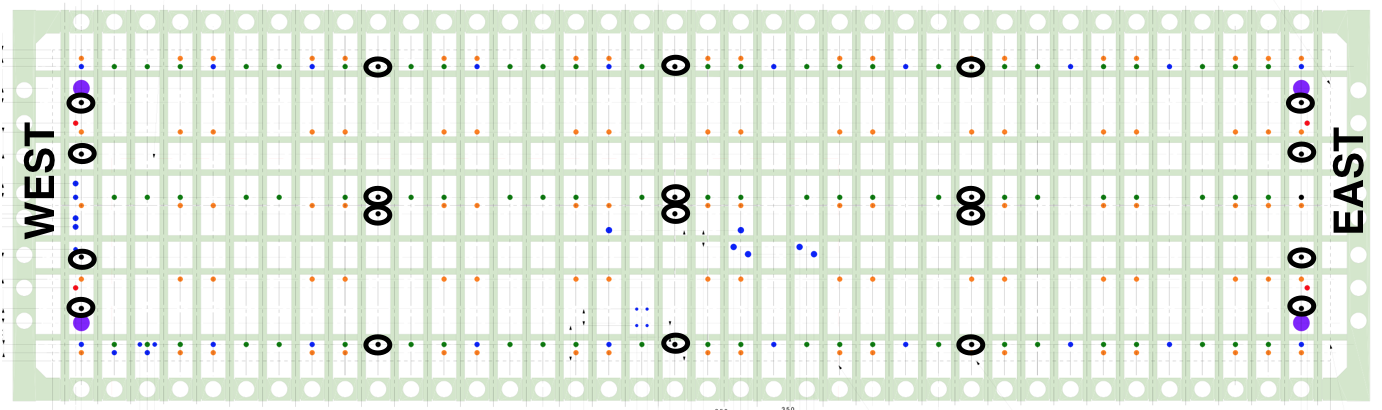
\includegraphics[height=2.0in]{FTmap.png}
%\caption{Top view of the \spmod %DUNE SP FD 
%cryostat showing various penetrations. Circles highlighted in black are multi-purpose calibration penetrations. The green dots are \dword{tpc} signal cable penetrations. The blue ports are cryogenic ports. The orange ports are \dword{dss} penetrations. The larger purple ports at the four corners of the cryostat are human access ports.}
%\label{fig:ftmap}
%\end{figure}

\begin{dunefigure}[Cryostat penetration map with calibration ports]{fig:FTmap}
{Top view of the \spmod %DUNE SP FD 
cryostat showing various penetrations. Circles highlighted in black are multi-purpose calibration penetrations. The green dots are \dword{tpc} signal cable penetrations. The blue ports are cryogenic ports. The orange ports are \dword{dss} penetrations. The larger purple ports at the four corners of the cryostat are human access ports.}
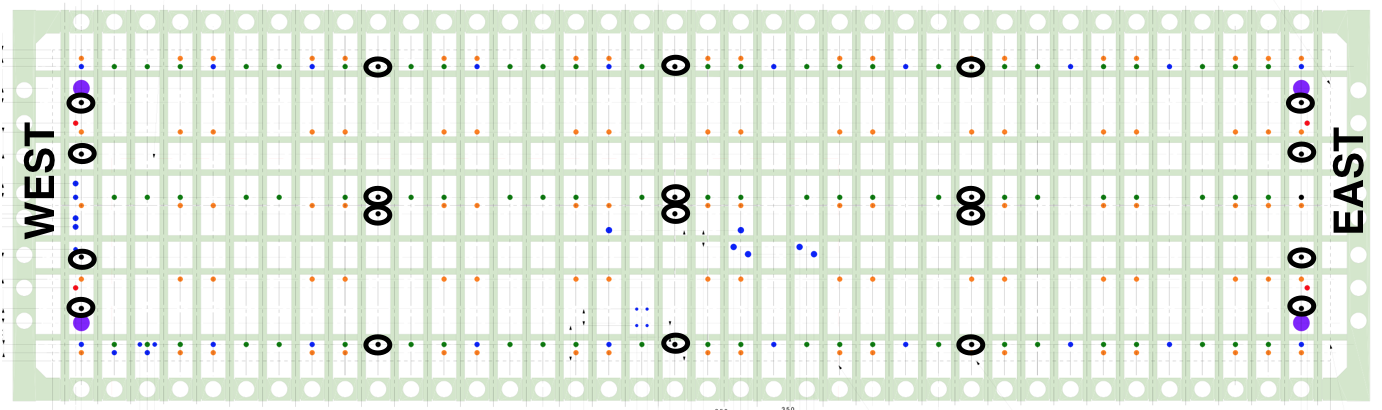
\includegraphics[height=2.0in]{FTmap.png}
\end{dunefigure}





Placement of these penetrations is largely driven by requirements for the ionization track laser. %and radioactive source system. 
The ports %that are %inwards 
toward the center of the cryostat are placed near the \dwords{apa} where the \efield is small \fixme{check} to minimize any risks due to the \dword{hv} discharge. For the far east and west ports, \dword{hv} is not an issue because they are located outside the \dword{fc} and the penetrations are located near mid-drift (location favorable to possible source deployment).
%to meet radioactive source requirements. 
%\fixme{The amendment above may need some work. I won't look at it until it's ready.}
Implementing the ionization track laser system as proposed in Section~\ref{sec:sp-calib-sys-las-ion} requires \num{20} feedthroughs at the four \dword{tpc} drift volumes; this arrangement allows lasers to be used for full volume calibration of the \efield and associated diagnostics (e.g., \dword{hv}). 

The distance between any two consecutive feedthrough columns in Figure~\ref{fig:FTmap} should be approximately \SI{15}{\m}, which is reasonable because experience from the \dword{microboone} laser system shows that tracks will propagate over that detector's full \SI{10}{\m} length. Assuming that the effects of Rayleigh scattering and self-focusing (Kerr effect) do not limit the laser track length, this laser arrangement could illuminate the full volume with crossing track data.  Please note that, at this time, the maximum usable track length is unknown, and it may be that the full \SI{60}{\m} \detmodule length could be covered by the laser system after optimization.




%%%%%%%%%%%%%%%%%%%%%%%%%%%%%%%%%%%%%%%%%%%%%%%%%%%%%%%
%\cleardoublepage

\section{Calibration Systems}
\subsection{Laser Calibration Systems}
\label{sec:sp-calib-sys-las}

%\fixme{KM: Some of the "possible measurements" read more like development plans.}


Through its effect on drift velocity, recombination, and lifetime, the \efield is a critical parameter for physics signals as it ultimately affects the spatial resolution and energy response of the detector. The primary purpose of a laser system is to provide an independent, fine-grained estimate of the \efield in space and time.
It would be extremely valuable to achieve measurements of electron lifetime with the laser system, but the feasibility of that is still under discussion. %and will be the goal of dedicated R\&D in the validation plan. 
The R\&D plan in \dword{protodune2} will address the feasibility of carrying out charge-based measurements which, if successful, would open up the possibility of using the laser to measure electron lifetime. So, except where specifically indicated, the rest of this section will focus on 
%be concerned with the 
drift velocity and \efield measurement.

\subsubsection{Physics Motivation}
Because it measures spatial distortions of straight tracks, the laser system actually measures the local drift velocity field directly and helps define the detector \dword{fv}, and this in itself is an important input for the \dword{lbl} analysis. 
%, and this is in itself an input to the analysis.
%Still,
However, it is still important to use information independent of the charge in order to disentangle effects like lifetime and recombination from \efield distortions. The laser system can do this, by using the position information to derive the \efield from the local velocity map, taking into account the colinearity between both vectors, and the relatively well studied relation between the magnitude of the drift velocity and the \efield, considering a temperature dependence (see~\cite{Li:2015rqa} and references [29, 45-58] therein). A laser system also has the intrinsic advantage of being immune to recombination effects, thus eliminating particle-dependent effects.  

Several sources may distort the \efield temporally  and/or spatially in the detector. Current simulation studies indicate that positive ion accumulation and drift (space charge) due to ionization sources such as cosmic rays or \Ar39 is small in the \dword{dune} \dword{fd}, causing \efield distortions of at most \SI{0.1}{\%}~\cite{bib:mooney2018}.
However, not enough is known yet about the fluid flow pattern in the \dword{fd} to exclude the possibility of stable eddies that may amplify the effect for both \single and \dual modules. %\dword{spmod} and \dword{dpmod}. 
This effect can be further amplified significantly in the \dword{dpmod} due to accumulation in the liquid of ions created by the electron multiplication process in the gas phase.
%due to ion accumulation at the liquid-gas interface. 
Additionally, other sources in the detector (especially detector imperfections) can cause \efield distortions. For example, \dword{fc} resistor failures, non-uniform resistivity in the voltage dividers, \dword{cpa} misalignment, \dword{cpa} structural deformations, and \dword{apa} and \dword{cpa} offsets and  deviations from flatness can create localized \efield distortions. These effects are presented in Figures~\ref{fig:efield_cpa_distortions_boyu2017} and \ref{fig:efield_resistorfailure_mooney2019}, showing the effect of a few \% on the \efield from \SI{2}{\cm} \dword{cpa} position tilts and %of 
up to \SI{4}{\%} from \dword{fc} single resistor failures.

\begin{dunefigure}[Impact on \efield of \dshort{cpa} position distortions]{fig:efield_cpa_distortions_boyu2017}
{Illustration of a possible distortion of the \dword{cpa} position~\cite{bib:yu2017a}, assuming a \SI{2}{\cm} swing, and its impact on \efield (right).}
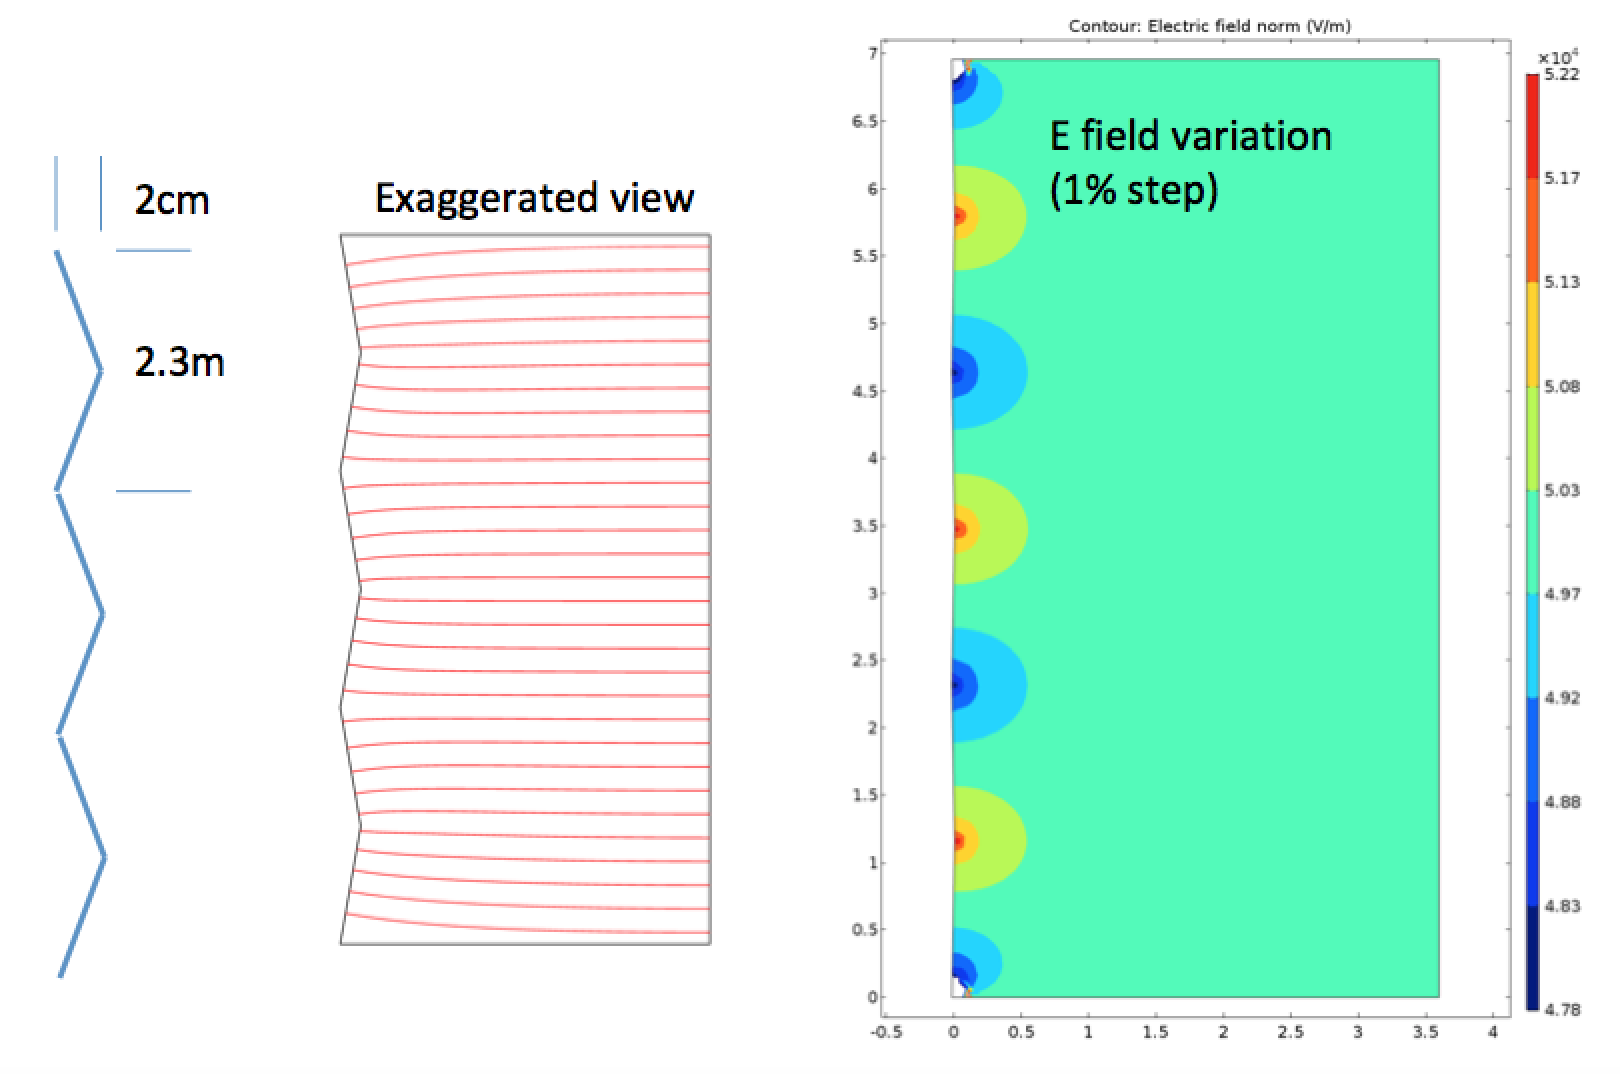
\includegraphics[width=0.8\textwidth]{efield_cpa_distortions_boyu2017.png}
\end{dunefigure}

\begin{dunefigure}[Impact on \efield of \dshort{fc} resistor failures]{fig:efield_resistorfailure_mooney2019}
{Impact on \efield magnitude distortions of a single \dword{fc} resistor failure~\cite{bib:mooney2019a}.}
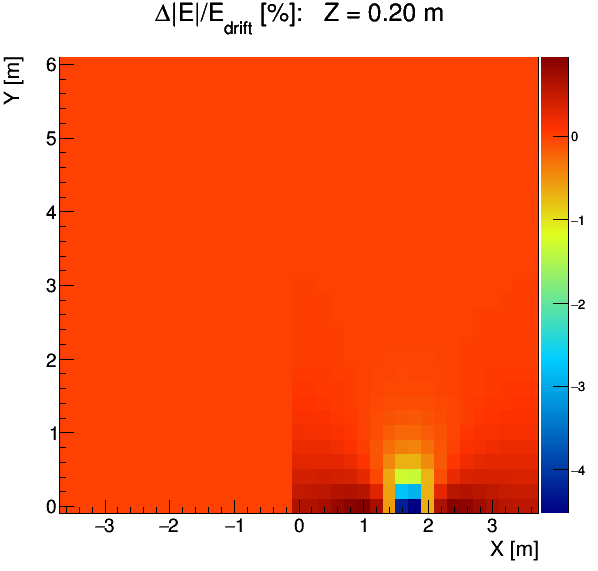
\includegraphics[width=0.5\textwidth]{efield_resistorfailure_mooney2019.png}
\end{dunefigure}

In both \single and \dual modules, %\dword{spmod} and \dword{dpmod} systems, 
a resistor failure will create significant, local \efield distortions that must be identified. In the \dword{dpmod}, %system, 
four resistors would have to fail to cause a failure across the \dword{fc} gap, but even one failure in the \dword{spmod} can have an effect; this may be partly, but not completely, mitigated by modifying the \dword{hv}. While the resistor failure will be detected temporally, its location in space is not possible to determine from slow controls monitoring data. Misalignments of detector objects or deformations may also create \efield distortions; while individual effects may be small, it is possible to have a combined, significant effect.
Each individual \efield distortion may add in quadrature with other effects, and can aggregate up to \SI{4}{\%} under certain conditions. Understanding all these effects requires in situ  measurement of \efield for proper calibration. 

Useful secondary uses of laser include alignment (especially modes that are weakly constrained by cosmic rays),
%; see Figure~\ref{fig:apacurtainalign}),
stability monitoring, and diagnosing detector performance issues
%failures 
(e.g., \dword{hv}).  
Misalignment may include physical deformation and/or rotations of objects within the detector. Given the expected low rate of cosmic ray events (about 3500/day/10-kt, inclusive) at the underground location, calibration with cosmic rays is not possible over short time scales. Even over long time scales, certain alignment directions  are difficult to assess with cosmic rays alone, such as distortions of the detector that preserve the gap widths and do not shift the \dwords{apa} in $x$ near the gaps relative to one another.
These distortions include global shifts and rotations in the locations of all detector elements, and crumpling modes where the edges of the \dwords{apa} hold together but angles are slightly different from nominal.   

%\fixme{SG: Can you check if you agree with this text below?}
With respect to electron lifetime, the preliminary results from \dword{pdsp} purity monitors and cosmic ray analyses indicate significant variations with time and space, both between monitors at different vertical coordinates (see \dword{tdr} \spchcisc), and between the regions inside and outside the \dword{tpc}. The possibility of carrying out such measurements with the ionization laser is therefore quite interesting. The ArgonTUBE experiment obtained lifetime measurements with laser~\cite{Ereditato:2013xaa} compatible with the cosmic ray ones, but it is not clear yet if this is possible at very large scales, since the modelling of the density of ionization charge created along the tracks presents challenges related to the previously mentioned self-focusing. Therefore the characterization of the ionization charge density from laser tracks will be an important goal of the development plan in \dword{protodune2}.


%A laser system also has the intrinsic advantage of being immune to recombination, thus eliminating particle-dependent effects.  





%%%%%%%%%%%%%%%%%%%%%%%%%%%%
\subsubsection{Requirements}
\label{sec:sp-calib-laser-req}



The energy and position reconstruction requirements for physics measurements lead to requirements on the necessary precision of the laser %calibration 
\efield measurement, its spatial coverage and granularity. The next sections discuss the rationale behind each requirement, which we take as the \dword{dune} specification.
%, with ALARA (or AHARA for the coverage) as goal.

\paragraph{\efield precision:}


In the \dword{lbl} and high-energy range, \physchlbl of this \dword{tdr}
%the \dword{dune} physics \dword{tdr} 
states that the calibration information must provide approximately \num{1} to \SI{2}{\%} understanding of normalization, energy scale and resolution, and position resolution within the detector.
Because a smaller \efield leads to higher electron-ion recombination and therefore a lower collected charge, distortions of the \efield can introduce
%are one of the possible causes of an 
energy scale bias. To connect this
%that requirement 
to a specification for the necessary precision of the \efield measurement, we note that, via recombination studies~\cite{bib:mooney2018}, we expect a \SI{1}{\%} distortion on \efield to lead to a \SI{0.3}{\%} bias on collected charge.
Because other effects will contribute to the lepton energy scale uncertainty budget, we consider a goal for the 
%calibration 
laser system to measure the \efield to a precision of $\sim$\SI{1}{\%} so that its effect on the collected charge is well below \SI{1}{\%}.
This is also motivated by consistency with the high level DUNE specification on field uniformity throughout the volume due to component alignment and \dword{hv} system, that 
%was 
is set at \SI{1}{\%}.
Together with two other high-level \dword{dune} specifications, the \dword{apa} wire spacing (\SI{4.7}{\mm}) and the front end peaking time (\SI{1}{\micro\s}), the effect of this \efield precision requirement on engineering parameters of the calibration laser system is discussed further %ahead, 
in Section~\ref{sec:sp-calib-sys-las-ion-meas}.

\paragraph{\efield measurement coverage:}

In practice, measuring the \efield  throughout the whole volume of the \dword{tpc} will be difficult, so we must establish a goal for the coverage and granularity of the measurement. 
Until a detailed study of the propagation of the coverage and granularity into a resolution metric is available, a rough estimate of the necessary coverage can be made as follows.

Assuming \SI{4}{\%} as the maximum \efield distortion %resulting 
that is %expectable 
expected from a compounding of multiple possible effects in the \dword{dune} \dword{fd} %as stated in the physics volume of the \dword{tdr},
as described in the previous section,
%(\cite{Abi:2018dnh}, page~4-53), 
we can then ask what would be the maximum acceptable size of the spatial region uncovered by the calibration system, if a distortion of that magnitude (systematically biased in the same direction) were present in that region. Our criterion of acceptability is to keep the overall \efield distortion, averaged over the whole detector, at the \SI{1}{\%} level. 
%, so then that 
To meet this requirement, the aforementioned spatial region should be no larger than \SI{25}{\%} of the total fiducial volume. Therefore, we aim to have a coverage of \SI{75}{\%} or more.

In addition, we need to consider that the method used to estimate \efield distortions is based on obtaining position displacement maps~\cite{bib:uBlaser2019}, and that the comparison between the reconstructed and true direction of a single track does not %univocally  %unequivocally
unambiguously determine a specific displacement map. Having tracks coming from different origins crossing in the same position is a direct way to eliminate that ambiguity, since the displacement vector is given simply by the vector connecting the intersections of the two reconstructed and the two true tracks. A joint iterative analysis of several close-by tracks is the default method for all other positions, but the system design should allow for the maximum possible number of positions %where there can be 
for crossing tracks from different beams.

\paragraph{\efield measurement granularity:}

Volume~\volnumberphysics~(\voltitlephysics) of this \dword{tdr} states that a \dword{fv} uncertainty of \SI{1}{\%} is required. 
This translates to a position uncertainty of \SI{1.5}{\cm} in each coordinate (see Chapter~\ref{ch:fdsp-apa}). 
In the $y$ and $z$ coordinates, position uncertainty is given mainly by the \dword{apa} wire pitch, and since this is about \SI{4.7}{\mm}, the requirement is met. In the drift ($x$) direction, the position is calculated from timing, and considering the electronics peaking time of \fepeaktime, the uncertainty should be even smaller.

The position uncertainty, however, also depends on the \efield, via the drift velocity. Because the position distortions accumulate over the drift path of the electron, it is not enough to specify an uncertainty on the field. We must accompany it by specifying the size of the spatial region of that distortion. For example, a \SI{10}{\%} distortion would not be relevant if it was confined to a \SI{2}{\cm} region and if the rest of the drift region was at nominal field.
%So 
Therefore, what matters is the product of [size of region] $\times$ [distortion]. Moreover, one can distinguish distortions into two types:
\begin{enumerate}
\item Those affecting the magnitude of the field. Then the effect on the drift velocity $v$ is also a change of magnitude. According to the function provided in \cite{Walkowiak:2000wf}, close to \SI{500}{\V\per\cm}, the variation of the velocity with the field is such that a \SI{4}{\%} variation in field $E$ leads to a \SI{1.5}{\%} variation in $v$.
\item Those affecting the direction of the field. Nominally, the field $E$ should be along $x$, so $E = E_L$ (the longitudinal component). If we consider that the distortions introduce a new transverse component $E_T$, in this case, this translates directly into the same effect in the drift velocity, which gains a $v_T$ component, $v_T=v_L  E_T/E_L $, i.e., a \SI{4}{\%} transverse distortion on the field leads to a \SI{4}{\%} transverse distortion on the drift velocity.
\end{enumerate}

Thus, a \SI{1.5}{\cm} shift comes about from a constant \SI{1.5}{\%} distortion in the velocity field over a region of \SI{1}{\m}. In terms of \efield, that could be from a \SI{1.5}{\%} distortion in $E_T$ over \SI{1}{\m} or a \SI{4}{\%} distortion in $E_L$ over the same distance.

%From ref.~\cite{Abi:2018dnh}, page~4-53, 
\efield distortions can be caused by space-charge effects due to accumulation of positive ions caused by \Ar39 decays (cosmic ray rate is low in \dword{fd}), or detector defects, such as \dword{cpa} misalignments (Figure~\ref{fig:efield_cpa_distortions_boyu2017}), \dword{fc} resistor failures (Figure~\ref{fig:efield_resistorfailure_mooney2019}), resistivity non-uniformities, etc.
%~\cite{Abi:2018dnh}. 
These effects added in quadrature can be as high as \SI{4}{\%}. 
%From ref. ~\cite{bib:mooney2018}, 
The space charge effects due to \Ar39~\cite{bib:mooney2018} can be approximately \SI{0.1}{\%} for the \dlong{sp} (\dshort{sp}), and \SI{1}{\%} for the \dshort{dp} (\dlong{dp}), so in practice these levels of 
%that kind of distortion 
distortions must cover several meters to be relevant.
Other effects due to \dword{cpa} or \dword{fc} imperfections can be higher because of space charge, but they are also much more localized. If we assume there are no foreseeable effects that would distort the field more than \SI{4}{\%}, and considering the worst case scenario (transverse distortions), then the smallest region that would produce a \SI{1.5}{\cm} shift is \SI{1.5}{\cm}/\num{0.04}~=~\SI{37.5}{\cm}. This provides a target for the granularity of the measurement of the \efield distortions in $x$ to be smaller than approximately \SI{30}{\cm}, with, of course, a larger region if the distortions are smaller. Given the above considerations, then a voxel size of \num{10}$\times$\num{10}$\times$\SI{10}{\cubic\cm} appears to be enough to measure the \efield with the granularity needed for a good position reconstruction precision. In fact, because the effects that can likely cause bigger \efield distortions are problems or alignments in the \dword{cpa} (or \dword{apa}) or in the \dword{fc}, it is conceivable to have different size voxels for different regions, saving the highest granularity of the probing for the walls/edges of the drift volume.









\subsubsection{Design}
\label{sec:sp-calib-sys-las-ion-des}
%\paragraph{Baseline design}

The design of the laser calibration system for \dword{dune} is largely based on the design of the system built for \dword{microboone}~\cite{microboone}, which in turn was based on several previous developments~\cite{Rossi:2009im,Zeller:2013sva,Ereditato:2014lra,Ereditato:82014tya}. A similar system was also built for \dword{captain}~\cite{Berns:2013usa} and in the near future, will be built for \dword{sbnd}~\cite{Antonello:2015lea}. Operation of the \dword{microboone} system has already taken place. A preliminary report was given in~\cite{bib:chen2018}, and more details on the data analysis are available in~\cite{bib:uBlaser2019}.
%\todo{link the reference once uB publishes the laser paper in 2019}

\paragraph{Design overview}
Ionization of \dword{lar} by laser can occur via a multiphoton process in which two-photon absorption~\cite{Badhrees:2010zz} leads the atom to the excited states band, and a third photon subsequently causes ionization. This can only occur with high photon fluxes, and so the lasers must provide pulse energies of \SI{60}{\milli\joule} or more within a few ns. Unlike muons, the laser beams do not suffer multiple scattering and travel along straight lines determined by the steering mirror optics. The basic measurement consists of %recording the laser beams 
generating laser ionization tracks in the \dword{tpc} and comparing the reconstructed tracks with the direction known from the steering hardware. 
An apparent curvature of the measured track is attributed to drift velocity, and therefore \efield, distortions (either in direction or magnitude).


While the Rayleigh scattering length for \SI{266}{\nano\m}  light is approximately \SI{40}{\m}, additional optics effects may limit the maximum practical range of laser beams of that wavelength to a distance smaller than that. Those can include the Kerr effect  due to the dependency of the refractive index on the \efield. In the presence of an intense field, such as that caused by the laser beam itself, the change in refractive index can lead to lensing, or focusing, that distorts the coherence of the beam\footnote{The Kerr effect is so far believed to be the cause of non-homogeneity of the ionization along the laser beam observed in \dword{microboone}, which prevents the use of the charge information. Its effect on the position measurement and \efield uncertainty has been studied by \dword{microboone}.}. 
%Still, 
Despite this, laser beams with lengths of \SI{10}{\m} in \dword{lar} have been observed in \dword{microboone}, and beams with \SI{20}{\m} lengths (possibly more) can be reasonably expected to obtain with a similar system.
This has determined the choice of locating five calibration ports in the cryostat roof at \SI{15}{\m} intervals along each of the four drift volumes of the \dword{spmod}, for a total of \num{20} ports. In fact, there are four ports just outside each of the \dword{fc} end-walls, and \num{12} ports located over the top \dword{fc}, close to the \dword{apa} of each drift volume, as shown in Figure~\ref{fig:calib-FTmap}. As is discussed further below, the number of ports %actually used 
currently assigned for the ionization laser system in the baseline design is \num{12}, a compromise between having the maximum possible coverage with crossing tracks and cost considerations.

\paragraph{Mechanical and optical design for a single port sub-system}

For each of %those 
the used calibration ports, a laser sub-system can be schematically represented by Figure~\ref{fig:uB_laser_schematic} (left) and consists of the following elements:
\begin{itemize}
    \item a laser box (see Figure \ref{fig:uB_laser_schematic}, right) that provides
    \begin{itemize}
        \item a Nd:YAG laser, with the fourth harmonic option providing \SI{266}{\nano\m} in intense \SI{60}{\milli\joule} pulses with about \SI{5}{\nano\s} width, with a divergence of \SI{0.5}{\milli\radian}. The Surelite SL I-10 laser\footnote{Amplitude Surelite\texttrademark{} https://amplitude-laser.com/wp-content/uploads/2019/01/Surelite-I-II-III.pdf} is a possible choice since it has been successfully used in the past in other experiments.
        \item an attenuator and a collimator to control the intensity and size of the beam;
        \item a photodiode that gives a \dword{tpc}-independent trigger signal;
        \item a low-power red laser, aligned with the UV laser, to facilitate alignment operations; and
        \item a Faraday cage to shield the surrounding electronics from the accompanying electromagnetic pulse. %EM \fixme{EM is defined as emergency management in the common glossary. Perhaps this should be spelled out? (Anne agrees and fixed.}
    \end{itemize}
    \item a feedthrough (see Figure \ref{fig:uB_laser_ft}, left) into the cryostat that provides
    \begin{itemize}
        \item the optical coupling that allows the UV light to pass through into the cryostat directly into the liquid phase, avoiding distortions due to the gas-liquid interface and the gas itself;
        \item a rotational coupling that allows the whole structure to rotate while maintaining the cryostat seal;
        \item a periscope structure (see Figure~\ref{fig:uB_laser_ft}; Right) mounted under the rotating coupling that supports a mirror within the \dword{lar};
        \item the additional theta rotation of the mirror accomplished by a precision mechanism coupled to an external linear actuator; and
        \item both the rotation and linear movements of the steering mechanism read out by precision encoders.
    \end{itemize}
    
\end{itemize}

\begin{dunefigure}[\dshort{microboone} laser calibration system schematics]{fig:uB_laser_schematic}
{Left: Schematics of the ionization laser system in one port~\cite{Antonello:2015lea}. Right: Schematics of the laser box~\cite{microboone}.}
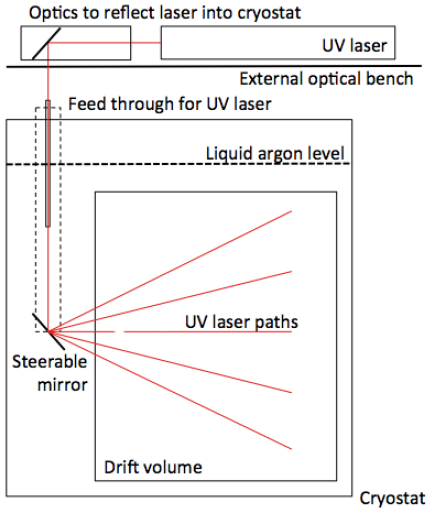
\includegraphics[width=0.45\linewidth]{uB_laser_schematic}
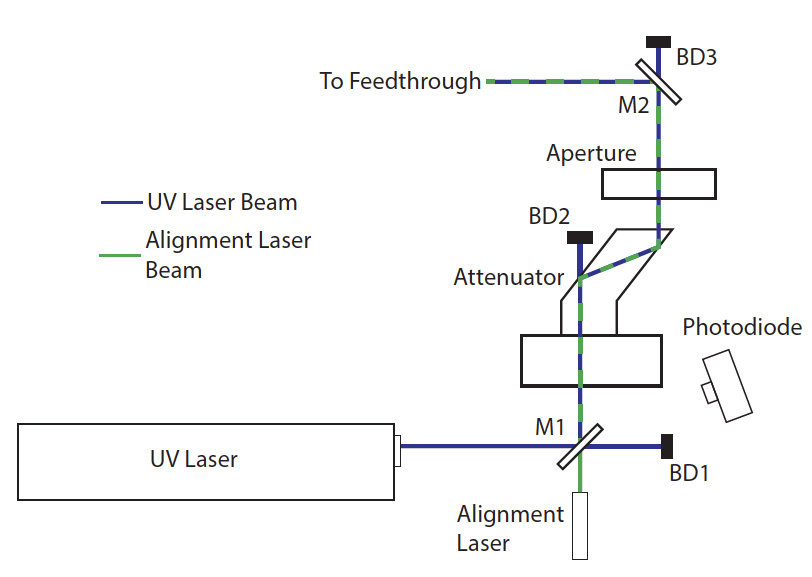
\includegraphics[width=0.5\linewidth]{uB_laser_box}
\end{dunefigure}

\begin{dunefigure}[\dshort{microboone} laser calibration system drawings]{fig:uB_laser_ft}
{CAD drawings of the \dword{microboone} laser calibration system~\cite{microboone}. Left: calibration port feedthrough. Right: laser beam periscope. %Both figures from~\cite{microboone}.
}
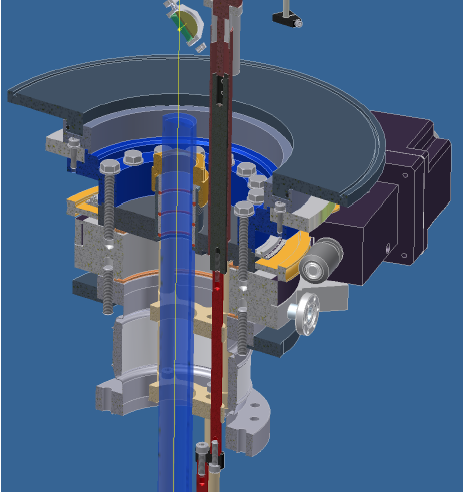
\includegraphics[width=0.49\linewidth]{uB_laser_ft}
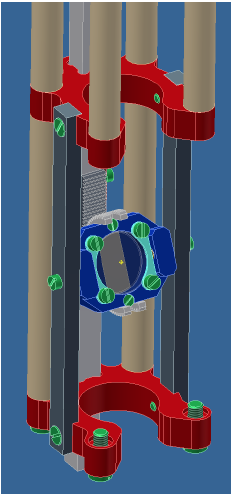
\includegraphics[width=0.248\linewidth]{uB_laser_periscope}
\end{dunefigure}

The goal of the mechanical design of the system is to achieve a precision close to that of the \dword{tpc} position measurements, so that no single factor dominates %in 
the overall systematics. The \dword{tpc} precision of about \SI{5}{\milli\m} in the $y$, $z$ coordinates is given primarily by the wire spacing of \uvpitch and \xgpitch. The precision of about \SI{2}{\milli\m} on the $x$ coordinate comes essentially from the \fepeaktime peaking time of the front-end electronics and the typical drift velocity (\driftvelocity).

The starting point of the laser beams is given by the position of the mirror in the periscope, which is known from construction drawings, warm surveys and cool down calculations. The angle of the beam is given by the angles ($\theta$, $\phi$) of the mirror, which are set by the periscope motors and read out by the encoders. 
For \dword{microboone}, reference~\cite{bib:chen2018} quotes a very good \SI{0.05}{\mrad} precision (\SI{0.5}{\milli\m} at \SI{10}{\m}) from the encoders alone, and an overall pointing precision of \SI{2}{\milli\m} at \SI{10}{\m}, driven mostly by beam size and divergence. In fact, with a \SI{0.5}{\mrad} divergence, we expect the beam to be \SI{5}{\milli\m} wide at \SI{10}{\m}.

In \dword{dune}, we aim to reach a similar precision. This will require a number of design and installation considerations: having encoders of similar high accuracy, carrying out surveys in various reference frames, and a capability to do location checks with a precision of about \SI{5}{\milli\m}  at \SI{20}{\m} from the beam origin. Therefore we aim to have a system that can locate the beam end point in few positions and attached to different references, at least one per drift volume and laser beam. 
%The goal of the laser system mechanical design and the laser location/positioning system is to achieve a precision close to that of the \dword{tpc} measurements, so that no single factor dominates the overall systematics.
%This corresponds to  providing the position of the beam to an accuracy of \SI{5}{\milli\m} with positioning systems located at about \SI{20}{\m} from the beam origin.
The independent laser beam location system is described in Section~\ref{sec:sp-calib-sys-las-loc}. 


\paragraph{Coverage estimations and top \dword{fc} penetration}
\label{sec:lasercoverage}

%\fixme{New sentences below. SG, please check and remove this.}
A crucial aspect of the design of the full array is the position of the periscope and the cold mirror with respect to the \dword{fc}, since its profiles can induce significant shadows and limit the beam's coverage. In order to address this aspect and motivate the design choices, we carried out a set of shadowing calculation studies.

Given that the \dword{fc} profiles are \SI{4.6}{\cm} wide with only a small \SI{1.4}{\cm} gap between them, the shadows produced if the laser source is located outside the \dword{fc} would be substantial. We estimate that the maximum angle at which beams can go through is about \ang{45}. Given the limitations of the region above the \dword{fc} (shown in Figure~\ref{fig:laser_topfc}, left), especially the geometry of the ground plane, it is likely that the mirror cannot be placed much higher up than \SI{40}{\cm} away from the \dword{fc}. 
With those assumptions, we have carried out a rough estimation of the fraction of voxels that would be crossed by any unblocked track. For simplicity, we are considering only a single vertical plane, so the coverage is actually overestimated since it does not consider the effect of the \dword{fc} I-beams, transverse to the \dword{fc} profiles.
Figure~\ref{fig:laser_topfc} (right) shows an example of those calculations. Assuming \SI{10}{\cm} voxels and no track directed at the \dword{apa}, the coverage is at most \SI{30}{\%}. Assuming \SI{30}{\cm} voxels and allowing all tracks directed at the \dword{apa}, the maximum coverage would be \SI{58}{\%}.

\begin{dunefigure}[View of top field cage and laser coverage estimation]{fig:laser_topfc}
{View of the top field cage (left) and laser 2D voxel coverage estimation for one drift volume (right).}
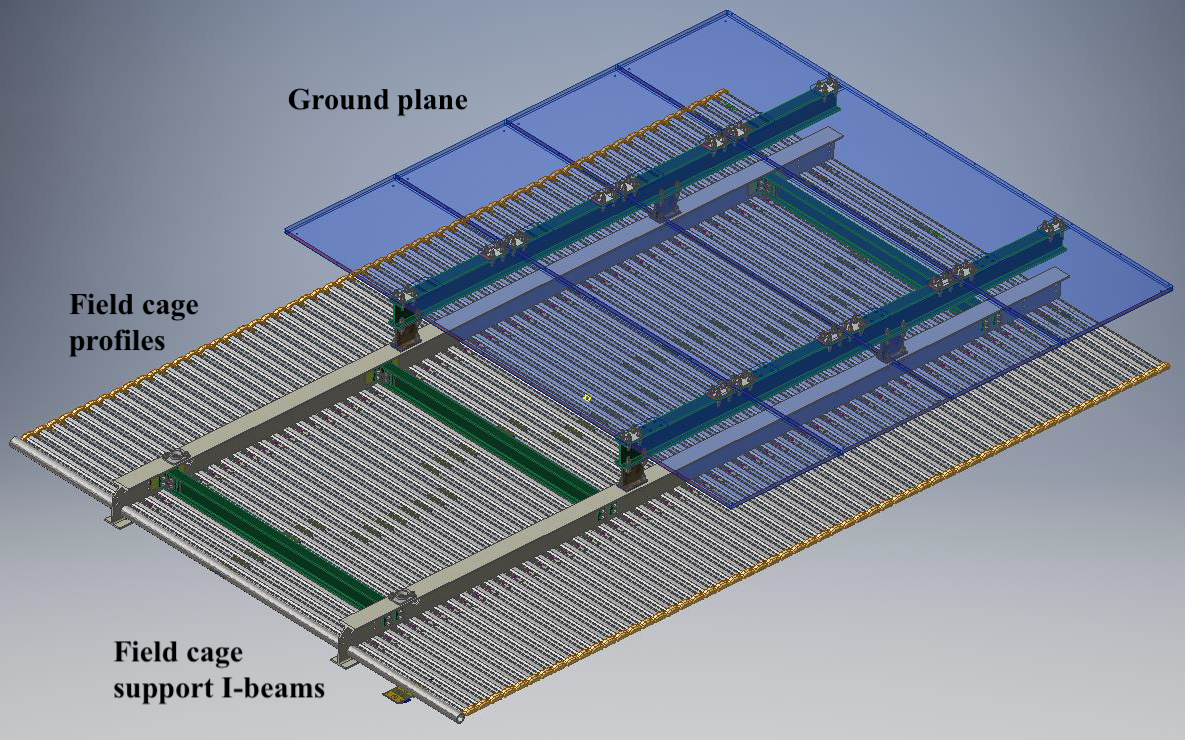
\includegraphics[width=0.7\linewidth]{calib-topFC_edit.png}
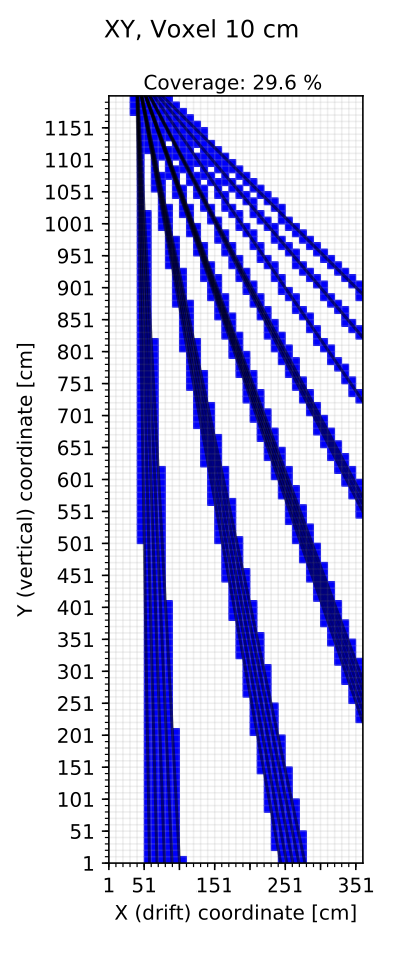
\includegraphics[width=0.29\linewidth]{calib-cov_XY_vox10_top_np1_noAPA_edit.png}
\end{dunefigure}

Penetration of the \dword{fc} would eliminate most of these shadows and allow for a practically unimpeded coverage. Depending on the depth of the periscope within the \dword{tpc}, some partial shadowing from the field cage support I-beam would still remain.
Figure~\ref{fig:laser_fcpenetration} shows a possible way to accomplish this for the top-of-TPC ports~\cite{bib:yu2019a}. A CAD model of the \dword{sbnd} laser calibration system periscope was used as 
%an example the design 
reference design for \dword{dune}. The \dword{sbnd} periscope, when rotating over its axis, requires a \SI{12}{\cm} diameter circular region free of impediments. In order to take into account a tolerance for the estimated \SI{0.3}{\%} shrinkage of the \dword{fc} at cryogenic temperatures, we chose an opening of three profiles, equivalent to \SI{18}{\cm}. 
%\fixme{New sentence below. SG, please check and remove this.}
Still, in order to minimize any risk associated with the presence of material close to the \dword{fc}, ongoing design studies will evaluate the feasibility of implementing vertically retractable periscopes, with a travel range sufficient for them to clear the top of the \dword{fc}. 

\begin{dunefigure}[Laser periscope penetrating the field cage]{fig:laser_fcpenetration}
{CAD drawing of one way the periscope could penetrate the \dword{fc}~\cite{bib:yu2019a}.}
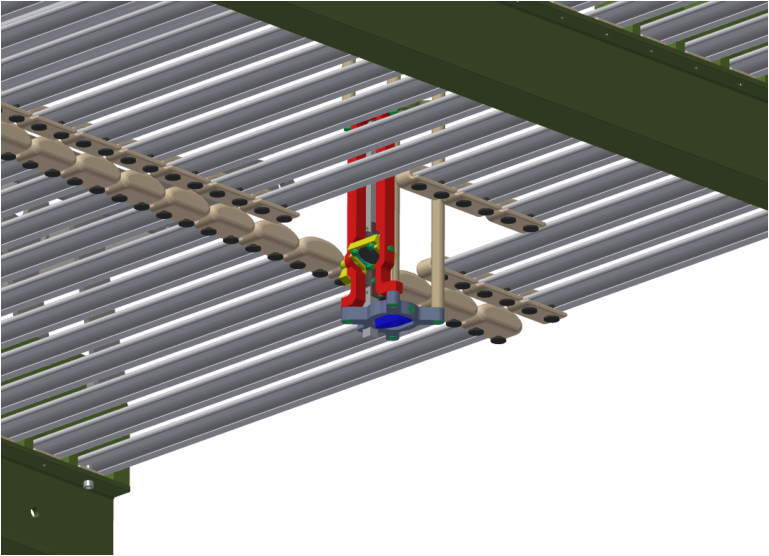
\includegraphics[width=0.6\linewidth]{laser_fcpenetration.pdf}
\end{dunefigure}

Simulations of the effect of \dword{fc} penetrations on the \efield were carried out~\cite{bib:yu2017b}, and are illustrated in Figure~\ref{fig:efield_penetration_boyu2017}. These have shown that the effect of a \SI{12x12}{\cm} opening (equivalent to two profiles), located at \SI{40}{\cm} (along the $x$ direction) from the \dword{apa}, is small and tolerable, with a maximum \SI{10}{\kilo\volt\per\cm} \efield caused by the opening and periscope.
These simulations need to be redone with a larger opening of \SI{18x18}{\cm}  (i.e., three profiles).
Still, if we were to choose, conservatively, to discard from the physics data analysis the volume within the \dword{tpc} determined by the periscope lateral size, a vertical penetration of \SI{10}{\cm}, and the full drift length (\SI{12x10x360}{\cm} = \SI{43}{\litre} for each of the \num{12} periscopes), it would represent only a very small fraction of \num{5e-6} of the full detector volume.

\begin{dunefigure}[Simulation of impact on \efield of \dshort{fc} penetration]{fig:efield_penetration_boyu2017}
{Simulation of the effect on the \efield of a laser periscope penetration of the \dword{fc}. In this case, an opening of only two profiles was considered.}
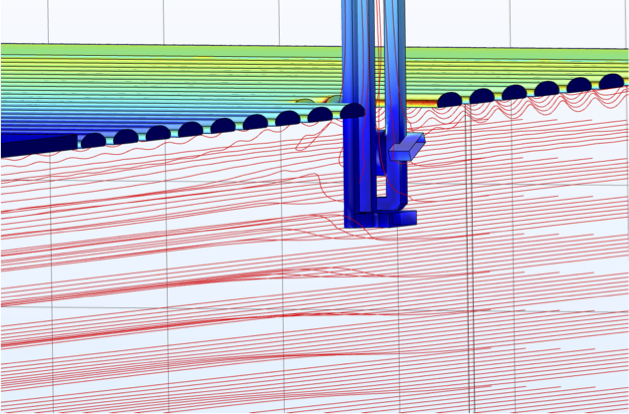
\includegraphics[width=0.6\linewidth]{efield_penetration_boyu2017.png}
\end{dunefigure}


\paragraph{Full array scope considerations}

As mentioned earlier (Section~\ref{sec:sp-calib-laser-req}), the system should allow for crossing laser beam tracks wherever possible. In order to %have 
collect them in the full \dword{spmod} volume, that would require using all the available \num{20} calibration ports. Since it is possible to use an iterative method to obtain displacement maps in regions where no crossing tracks are available, 
%for cost compromise reasons 
to minimize the overall cost of the system, the baseline design will use only the \num{12} central ports, providing crossing tracks in essentially \SI{50}{\%} of the detector volume. 
%Actually, 
In addition, for the six most central ports, close to the central \dword{apa}, the distance between them is small enough that we can consider having the same laser box serve two feedthroughs to reduce the costs associated with the laser and its optics. In that case, the total number of lasers needed would be nine.

Usage of the end-wall ports, which are not %over 
on top of the \dword{tpc}, is therefore not part of the baseline design, and is considered only as an alternative in Section~\ref{sec:sp-calib-laser-alter}. A coverage calculation for possible end-wall periscopes, taking into account the shadowing of both the \dword{fc} profiles and the support beams, gives a maximum of \SI{56}{\%} coverage for \SI{30}{\cm} voxels (allowing all tracks directed at the \dword{apa}). In this case the laser beams would enter the \dword{fc} laterally and \dword{fc} penetration would be harder to consider, so an alternative mechanical design aimed at improving the coverage, is considered in Section~\ref{sec:sp-calib-laser-alter}.



%a \SI{266}{\nano\m} laser would be mounted on the top of the cryostat, and service two adjacent feedthroughs. A steerable head and fiber interface would be mounted in the feedthrough, which is coated in a insulator. Two options are under investigation: (1) the \dword{fc} (but not the \dword{gp}) is penetrated, and (2) the \dword{fc} is not penetrated. In the former case, the \dword{fc} penetration has been shown to create a small distortion to the E-field, for the benefit of full volume E-field mapping. When the \dword{fc} is not penetrated, the laser shines through the \dword{fc} tubes, producing some regions that are not mappable by the laser. Unlike the ports that are inwards of the cryostat, the lasers through penetrations that are outside the \dword{fc} on the far east and west side of the cryostat will not penetrate the field cage. The photo-electron system would include a fiber and no steering; the necessity of penetrating the \dword{fc} is unlikely but has not been assessed yet.

A scan of the full detector using \num{10}$\times$\num{10}$\times$\SI{10}{\cubic\cm}
volume elements would require a number of tracks approximately \num{8e5} 
%would 
and can take about three days. Shorter runs could be done to investigate specific regions. The sampling granularity, and therefore the amount of data taken, depends on \dword{daq} requirements. In fact, even to be able to record the desired \num{8e5} tracks, a dedicated data reduction algorithm must be devised, so that only a drift window of about \SI{100}{\micro\s}
of data is recorded, and the position of that window depends on the beam position and direction and which wires are being read out. More details on this are given in Section~\ref{sec:sp-calib-daqreq}.

%The direct ionizing laser system may also be used to create \phel{}s from the cathode, even under low power operation.

%% JM %% end % from early IDR version




%%%%%%%%%%%%%%%
%\subsubsubsection{Possible Measurements}
\subsubsubsection{Measurement Program}
\label{sec:sp-calib-sys-las-ion-meas}

This section describes the methods used to measure 
%drift velocity and \efield 
parameter maps and their expected precision, given the design outlined above.

\paragraph{\efield and drift velocity measurement}
The method for \efield measurement is based on the measurement of apparent position displacements of the straight laser tracks. The laser produces straight tracks with a known starting position and direction. If, when reconstructed under the assumption of uniform and homogeneous drift velocity, any deviations from that are observed, they are attributed to \efield distortions. 

The first step in the analysis~\cite{bib:uBlaser2019} is to obtain a field of position displacements by comparing the known and reconstructed tracks. If two crossing tracks are used, the displacement vector is simply given by the vector connecting the point where the reconstructed tracks cross and the point where the known tracks cross. However, since those displacements can vary both in direction and magnitude, there will be ambiguity in that determination if only one track is used in a given spatial region. An iterative procedure was developed by the \dword{microboone} collaboration~\cite{bib:chen2018,bib:uBlaser2019} to obtain a displacement map from a set of several non-crossing tracks from opposite directions. Following this, a set of drift velocity field lines, which are the same as \efield lines, can be obtained from the displacement map, assuming that all charge deposits along a field line will be collected in the same position. Using the relationship between \efield and drift velocity~\cite{Li:2015rqa,Walkowiak:2000wf}, we can then also obtain the magnitude of the \efield.

Since the observed position distortion in one location depends on \efield distortions in many locations along the drift path, this method of analysis clearly requires the acquisition of data from many different tracks crossing each detector drift volume at many different angles. 

As already indicated in the previous section (section~\ref{sec:sp-calib-sys-las-ion-des}), the pointing precision will be on average \SI{2}{\milli\m} (at average distances of \SI{10}{\m}), and the \dword{tpc} precision is \SI{2}{\milli\m} in $x$ and \SI{5}{\milli\m} in $y$, $z$. Conservatively taking those in quadrature, we get $\sigma_x$ =  \SI{3}{\milli\m} and $\sigma_{yz}$ = \SI{5.4}{\milli\m}.
If we would use only one track per direction, in regions of size $l$ = \SI{300}{\milli\m}, we would therefore be sensitive to drift velocity field distortions of $\sigma /l$, i.e., \SI{1}{\%} in $x$ and \SI{1.8}{\%} in $y$, $z$. 

In order to estimate the \efield precision, we must distinguish between the $x$ and $y$, $z$ coordinates. To first order, distortion in $y$, $z$ do not affect the magnitude of the field, and so the relative distortions on \efield are equal to the relative distortions of the velocity. Along $x$, we must consider the relation between the magnitudes of the drift velocity and \efield. Using the formula from~\cite{Li:2015rqa,Walkowiak:2000wf} we can see that, at \spmaxfield, a \SI{1}{\%} change in \efield leads to a corresponding change of \SI{0.375}{\%} in drift velocity. We therefore reach the values of \SI{2.7}{\%} ($=1./0.375$) in $x$ and \SI{1.8}{\%} in $y$, $z$ for a conservative estimate of \efield precision using a single track per direction. 

This is a conservative estimate because it does not take into account the fact that the centroid of the beam should be known better than its full width, and because it is based on the assumption of a single track per direction.  
As observed in \dword{microboone}~\cite{bib:uBlaser2019}, using several tracks improves the precision, and in most of the volume an accuracy of \SI{1}{\%} was reached so the amount of statistics needed to reach \SI{1}{\%} will be an important question to address in the development plan. 



On one side, this gives us an ultimate limit to the \efield precision achievable with the laser system, but on the other side, since these \dword{tpc} precision considerations apply to physics events also, it tells us that an \efield precision much better than \SI{1}{\%} should not have an effect on the physics.



\paragraph{Charge-based measurements}

Electron drift-lifetime~\cite{bib:uBlifetime, Antonello:2014eha} is the parameter that governs the dependence of the amount of collected charge on the drift time. A possible measurement of electron drift-lifetime would therefore require a very good control over the charge profile of the ionization laser tracks. This was achieved in a small scale experiment that measured lifetime with laser beams~\cite{Ereditato:2013xaa}, but is harder with longer distances. The charge produced by the laser tracks along its path depends on distance because the light intensity is reduced due to beam divergence and scattering, as well as non-linear effects such as the self-focusing, or Kerr effect. For this reason, the first steps in any laser-based charge measurement are a fine-tuning of the laser intensity in order to reduce self-focusing to a minimum, and ``charge profile calibration scan'' which consists of acquiring tracks parallel to the \dword{apa}. In order to get good statistical precision, several tracks could be acquired, in the same or different direction, but always parallel to the \dword{apa} in order to factorize out any effect from electron drift-lifetime. This set of data provides a calibrated laser beam charge profile that can then be used to analyse and normalize the measured charge profile from tracks that do have an angle with respect to the \dword{apa} and therefore span different drift times.

As for electron-ion recombination, since the $dE/dx$ for laser beams is much smaller than for charged particles, the effect should also be much smaller. However, that small effect has been observed~\cite{Badhrees:2010zz}, so a similar method than described above could be used to evaluate any dependence of the electron-ion recombination factor on the angle $\phi$ between the track and the electric field, that is predicted in some models~\cite{Acciarri:2013met}. This would entail taking data with tracks as parallel as possible to the \efield, in order to enhance the angular dependence term on the recombination expression (that goes with $1/sin \phi$), and to compensate for the smaller $dE/dx$ for laser beams.






\subsection{Laser positioning system}
\label{sec:calib-laser-pos}

Since the precision of the \efield measurement is heavily reliant on a precise knowledge of the laser beam tracks, an independent measurement of their direction for some specific positions, is required. The laser positioning system addresses this requirement.
%\subsubsection{Physics Motivation}
While the direction of the laser beam will be very well known based on the reading from the encoders on the laser beam steering mechanism,  residual uncertainty or unpredictable shift in the pointing direction will remain. 
%Having 
Keeping in mind the long length of the ionization track of more than \SI{15}{\m}, even a small offset in the pointing direction can lead to vastly different ionization track location, especially close to the end of the track. Such inaccuracies will directly impact the ability to precisely calibrate any variations in the \efield.

\subsubsection{Design}

The laser positioning system (LPS) is designed to address the problem of precise and accurate knowledge of the laser track coordinates. %University of Hawaii group has 
Two complementary systems are planned, one based on PIN diodes and another based on mirrors.

\paragraph{Pin-diode system for laser positioning}

A system based on PIN diodes 
%(consisting of 1$\times$3) array 
was built for the miniCAPTAIN experiment \fixme{needs ref} and the installed version is visible in the photo of the miniCAPTAIN TPC as shown in  Figure~\ref{fig:LPS_miniCAPTAINlabeled}.  

%\begin{figure}[htb!] 
%\centering 
%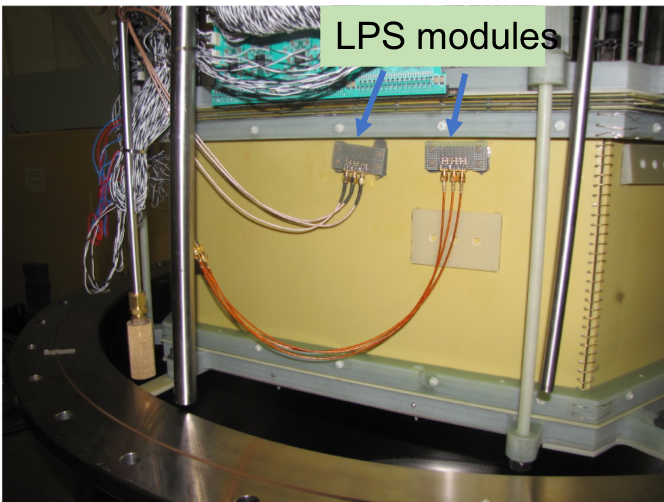
\includegraphics[width=0.6\linewidth]{LPS_miniCAPTAINlabeled.png} 
%\caption{Photo of the miniCAPTAIN TPC with two LPS modules glued on the outside to detect laser beam spot location via fluorescence of the TPC FR4 wall when illuminated by the laser beam.}
%\label{fig:miniCAPTAIN} 
%\end{figure}

\begin{dunefigure}[Laser positioning system modules in the miniCAPTAIN TPC]{fig:LPS_miniCAPTAINlabeled}
{Photo of the miniCAPTAIN TPC with two LPS modules glued on the outside to detect laser beam spot location via fluorescence of the TPC FR4 wall when illuminated by the laser beam.}
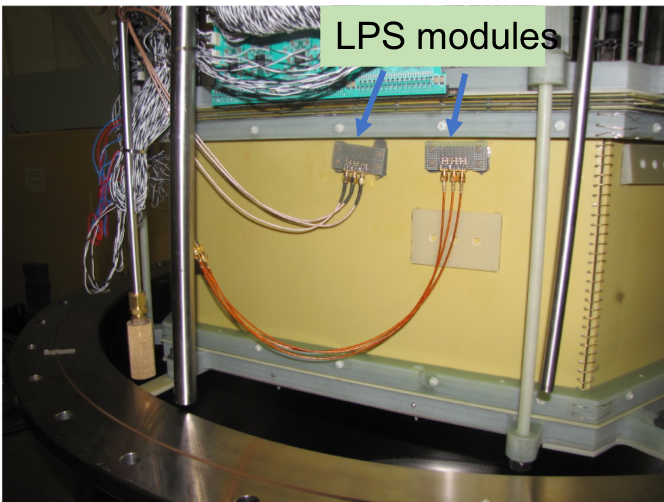
\includegraphics[width=0.6\linewidth]{LPS_miniCAPTAINlabeled} 
\end{dunefigure}

The LPS consists of groups of \num{9} PIN diodes, operating in passive, photovoltaic mode. These are GaP diodes whose sensitivity range extends down to  \SI{200}{\nano\m} wavelength --- thus detecting \SI{266}{\nano\m} light is straightforward. Figure~\ref{fig:GaP_diode_room_temp} shows signal detected at room and cryogenic temperatures. PIN diode was illuminated by the \SI{266}{\nano\m} light from the Nd:Yag
laser in the lab 
%(in the lab at University of Hawaii) 
set at lowest possible setting for minimal power.  \fixme{add lps to gloss}

PIN diodes are placed at the bottom of the cryostat and receive light passing through the gaps between the field cage profiles to minimize interference with the field cage. Drawings of one such group of PIN diodes are shown in Figure~\ref{fig:GaP_assembly}. With the group of \num{9} photodiodes, one cannot only detect the beam but also crudely characterize its profile, giving a more precise location of the central beam pulse axis.


%\begin{figure}[htb!] 
%\begin{minipage}[b]{0.47\textwidth}
%\centering 
%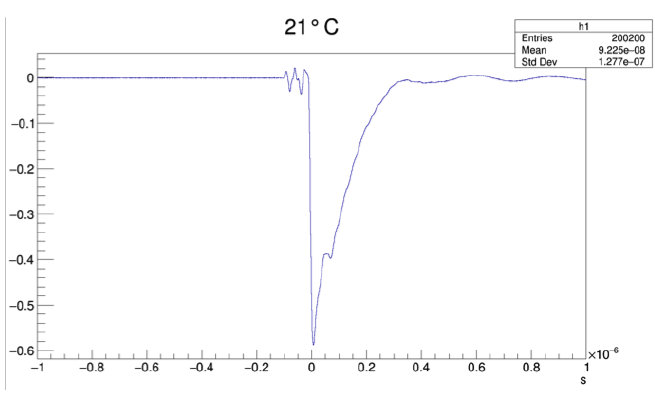
\includegraphics[width=0.95\linewidth]{GaP_diode_room_temp.png} 
%\caption{Signal from the GaP pin diode. The signal was a result of illumination of the PIN diode face with a 266\,nm laser at room temperature.}
%\label{fig:LPS1} 
%\end{figure}
%\end{minipage}
%\hfill
%\begin{minipage}[b]{0.47\textwidth}
%\begin{figure}[htb!] 
%\centering 
%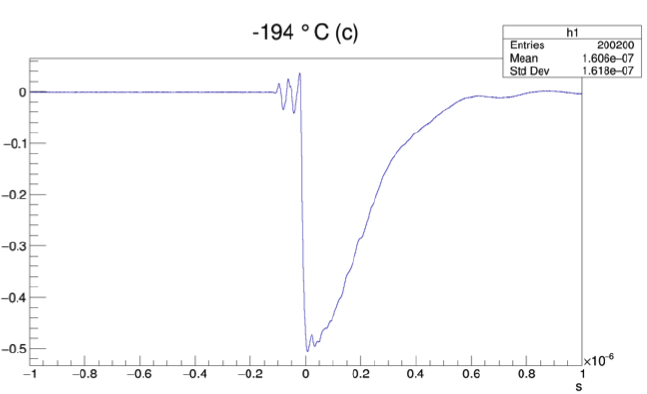
\includegraphics[width=0.95\linewidth]{GaP_diode_cryo_temp.png} 
%\caption{Signal from the GaP pin diode. The signal was result of illumination of the PIN diode face with a 266\,nm laser at cryogenic temperature.}
%\label{fig:LPS2} 
%\end{minipage}
%\hfill
%\end{figure} 


%\begin{figure}[htb!] 
%\begin{minipage}[b]{0.47\textwidth}
%\centering 
%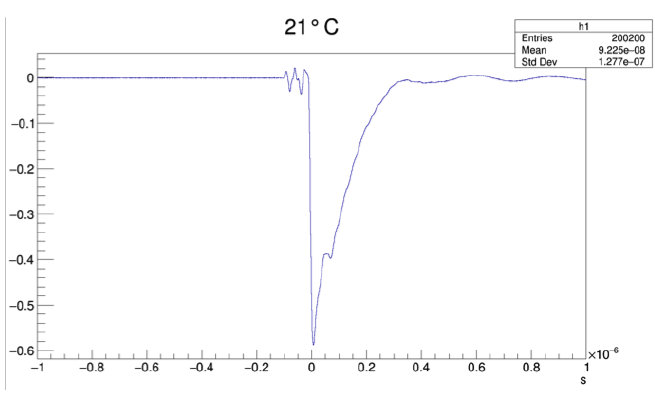
\includegraphics[width=1.0\linewidth]{GaP_diode_room_temp.png} 
%\caption{Signal from the GaP pin diode. The signal was a result of illumination of the PIN diode face with a 266\,nm laser at room temperature.}
%\label{fig:LPS1} 
%\end{minipage}
%\hfill
%\begin{minipage}[b]{0.47\textwidth}
%\centering 
%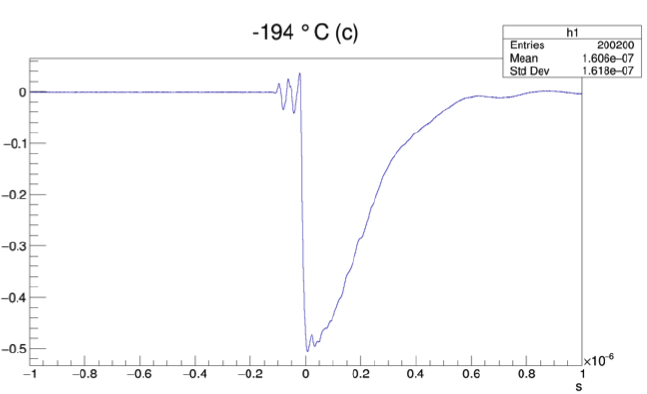
\includegraphics[width=1.0\linewidth]{GaP_diode_cryo_temp.png} 
%\caption{Signal from the GaP pin diode. The signal was result of illumination of the PIN diode face with a 266\,nm laser at cryogenic temperature.}
%\label{fig:LPS2} 
%\end{minipage}
%\hfill
%\end{figure} 


\begin{dunefigure}[Signal from the miniCAPTAIN laser positioning system at room and cryogenic temperatures]{fig:GaP_diode_room_temp}
{Signal from the miniCAPTAIN laser positioning system GaP PIN diode. The signal was a result of illumination of the PIN diode face with a \SI{266}{\nano\m} laser at room (left) and cryogenic (right) temperatures.}
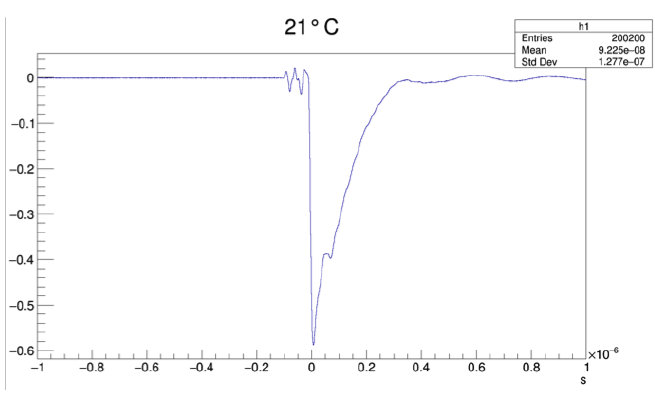
\includegraphics[width=0.47\linewidth]{GaP_diode_room_temp.png} 
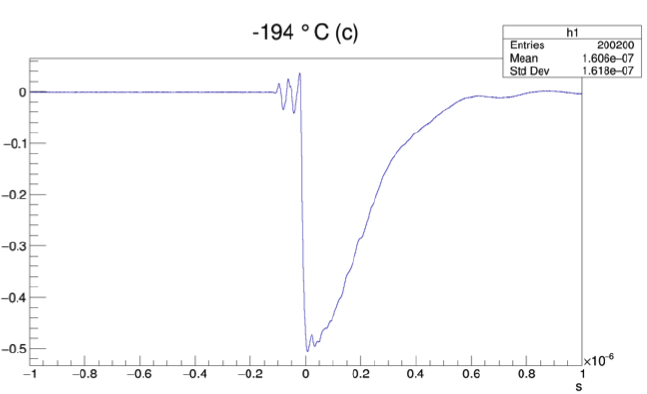
\includegraphics[width=0.47\linewidth]{GaP_diode_cryo_temp.png} 
\end{dunefigure}



\begin{dunefigure}[Cluster assembly of the miniCAPTAIN laser positioning system]{fig:GaP_assembly}
{(Left) LPS cluster mounted on the opposite wall from the laser periscope to detect and accurately determine the end point of the laser beam. (Right)
Profile of the LPS group mounted on the PCB. GaP diodes come with pins that use pair of twisted wires to transport the signal.
}
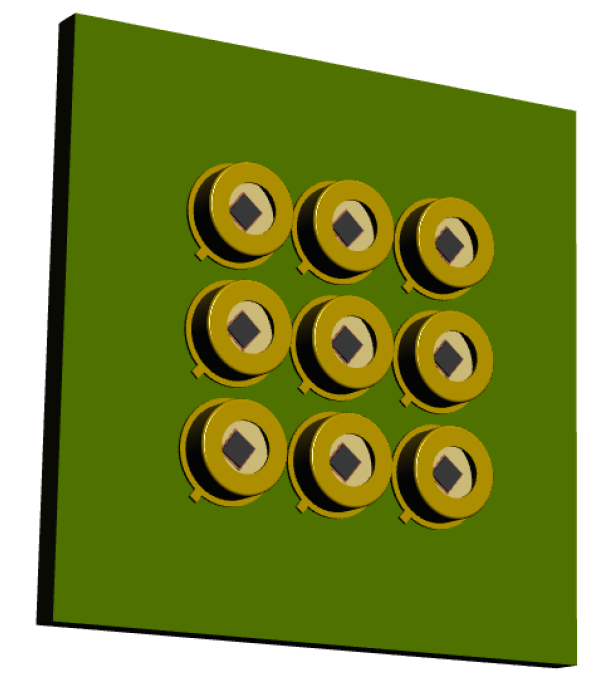
\includegraphics[width=0.47\linewidth]{GaP_assembly.png} 
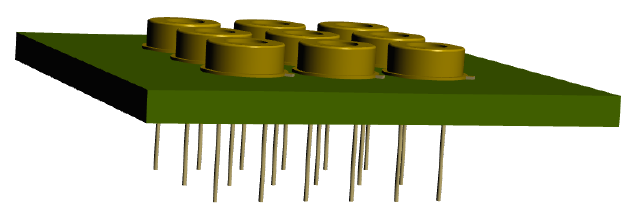
\includegraphics[width=0.47\linewidth]{GaP_assembly_profile.png} 
\end{dunefigure}


There will be one LPS pad per laser. The laser would always send the first pulse in the direction of the LPS before proceeding into a calibration sequence. 
%The electronics used to collect signals from the LPS will be provided by \dword{cisc}.\todo{CISC doesn't provide electronics. SG emails Jelena to clarify this.}


\paragraph{Mirror-based beam positioning system}

In addition to the pin-diode system, we will also have clusters of small mirrors, that allow the measurement of the beam end position via its reflections.

Figure~\ref{fig:laser_mirror_positioning} shows a conceptual sketch, with a cluster of 6 mirrors located close to each other, but with different angles. When the beam hits one of the mirrors, it will be reflected back into the TPC, and the reflection angle unambiguously identifies which mirror was actually hit. With small mirrors, of \SI{5}{\milli\m} diameter, the required positioning precision would be met, if these mirrors are place at distances of over \SI{10}{\m}. The preferred location is therefore at the bottom \dword{fc}. Since the cluster can be small (a few cm), it can fit inside the \dword{fc} profiles. For each drift volume segment seen by two lasers, we plan to install at least two clusters, for redundancy, so the total number of clusters would be \num{32}. 

The simplest solution would be to have the reflecting surface be polished aluminum, so that the cluster could be a single block. Tests will have to be made for the actual reflectivity of the (oxidized) surface. An alternative could be the use of small dielectric mirrors.

\begin{dunefigure}[Mirror-based laser beam positioning system]{fig:laser_mirror_positioning}
{View of the mirror cluster for the beam positioning system, inserted within the \dword{fc} profiles~\cite{bib:yu2019a}.}
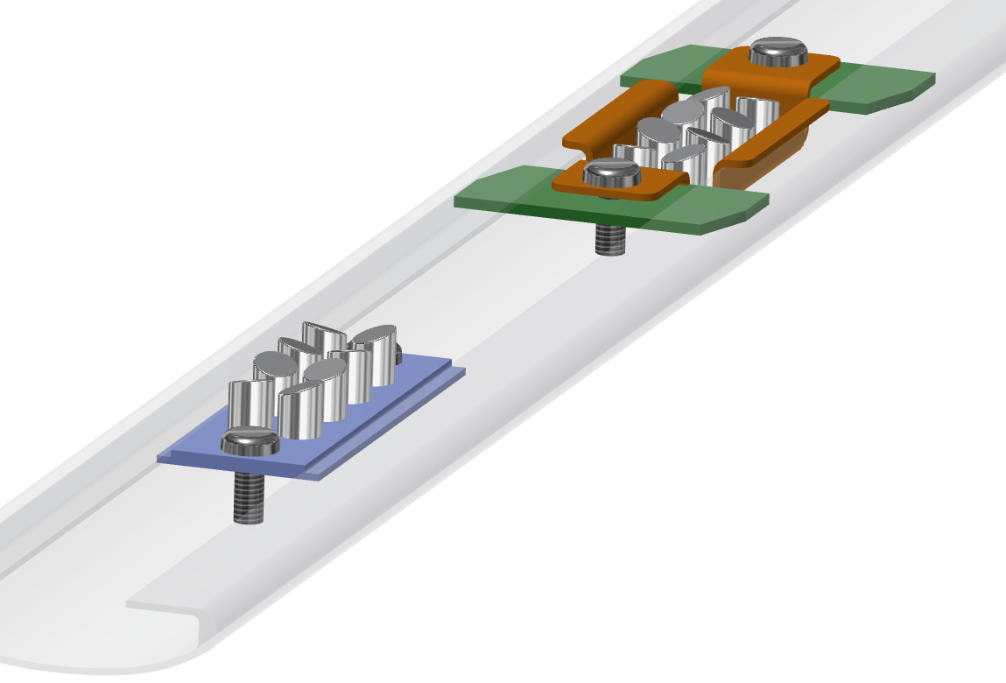
\includegraphics[width=0.7\linewidth]{laser_mirror_positioning.pdf}
\end{dunefigure}

\subsubsection{Development plan}
 Further optimization of the LPS assembly to reduce electronic noise and cross-talk is required. Also, the size and shape of the cluster that would best collect the light coming through the field cage gaps needs to be optimized.  Another important aspect is durability of the system that will require extensive running in the cryogenic conditions with  a large number of cool-downs to validate GaP for extended use in DUNE. Finally, alternatives to GaP diodes such as SiPMs are under consideration. While SiPMs require power, their sensitivity to single photons makes them a desirable candidate for low light signals and more accurate beam direction reconstruction. 

















%\fixme{KM: I think I got the number of subsections wrong for the positioning system, it should be under the ionization laser.}

\subsection{Photoelectron Laser System}
\label{sec:sp-calib-sys-las-pe}
%\subsubsection{Physics Motivation}
%\label{sec:sp-calib-sys-las-pe-phys} 
Well localized electron sources represent excellent calibration tool for study of the electron transport in the \dword{lartpc}, identification of the inhomogeneities in the TPC \efield in all directions, and precise determination of the electron drift velocity. Verification and calibration of the \efield distortions play an important role in particle vertex reconstruction and identification and affects the associated systematic errors, leading to increased rate of mis-identification and poorer energy reconstruction. Photoelectron laser can provide well localized electron sources on the cathode at predetermined locations leading to improved characterization of the \efield, and consequent reduction of detector instrumentation systematic errors. Also, photoeletron laser system, being a simpler system operationally compared to the ionization laser system, can be used as a wake-up system to quickly diagnose if the detector is alive. This is especially important due to the low cosmic ray environment in the detector underground. 

\subsubsection{Design}
\label{sec:sp-calib-sys-las-pe-des}

In order to produce localized clouds of electrons using a photoelectric effect, small aluminum discs or thin discs with evaporated gold film, will be used as targets. As stated in reference~\cite{Li:2016ods}, gold film can be just \SI{22}{\nano\m} thick. Several photoelectric strips will complement the circular targets to calibrate the rate of transverse diffusion in \dword{lar}. Based on the experience from T2K and BNL \dword{lar} test-stands~\cite{Li:2016ods}, \SIrange{8}{10}{\milli\m} diameter targets are sufficient. Targets will be placed on the cathode and distance between the dots will be determined based on the calibration needs and simulation outcomes. Nominally, dot spacing should be \SI{1}{\m} with photocathode strips every \SI{5}{\m}. The photoelectric dots and strips layout will be further refined based on the calibration requirements and performance simulation results. It will be essential to conduct a survey of the photocathode disc locations on the cathode  after installation and prior to detector closing. In this way, the absolute spatial calibration of the electric field can be achieved. 
At \SI{266}{\nano\m} Nd:Yag quadrupled wavelength, the single photon energy of \SI{4.66}{\eV} is sufficient to generate photoelectrons from aluminum, but not from gold, that requires two-photon absorption and therefore higher intensities.
%At S\I{266}{\nano\m} Nd:Yag quadrupled wavelength, the photon energy of\SI{4.66}{\eV} is sufficient to generate photoelectrons from both aluminum and gold. 
While aluminum has a lower associated cost, gold film surface is easier to protect from contamination. 
%A couple of hundred electrons 
%A couple of thousand electrons 
A few thousand electrons are expected per spill from each dot. The laser beam will be coming from the anode injection points, used as sources, guided to injection points via cryogenic optical fibers with defocusing elements on the other end. 

If aluminum is chosen, then single photon absorption is enough and a lower laser intensity is required, opening up the 
%Much lower energy required for photoelectric laser, opens up the
possibility for a rather efficient calibration of each drift volume. Namely, laser pulse can be distributed to two drift volumes at the time in order, while illuminating the entire cathode assembly. Since the photoelectron clouds from different dots are very well localized, calibration of the \efield distortion in the entire drift volume can be done with a single laser trigger, if the light is distributed to all injection fibers for one drift volume. 

The photoelectron system will use the same lasers used for argon ionization. Stability of the laser pulses will be monitored  with  power meter. Dielectric mirrors will guide the laser light to injection points, but fraction of the light will be transmitted instead of reflected to the power meter behind the mirror. 

Laser will also send forced trigger signal to the DAQ based on the photodiode that will be triggered on the fraction of the light passing through the dielectric mirror. Special mirrors reflective to \SI{266}{\nano\m} light will be utilized. 

The photoelectron system will require the following tasks to complete the design: test the mounting of the targets on the cathode plane assembly; survey of the dots position to the required level of precision; and  study thickness of the target and photoelectron yield as a function of target choice, laser power and attenuation of the laser light in the optical fibers.

%The first thing that needs to be tested is the mounting of the targets on the cathode plane assembly. In addition, survey of the dots position to the required level of precision is needed. Thickness of the target and photoelectron yield as a function of target choice, laser power and attenuation of the laser light in the optical fibers.

\subsubsection{Measurement Program}
\label{sec:sp-calib-sys-las-pe-meas}

Photoelectron systems have been used in other experiments to diagnose electronics issues by using the known time period between triggered laser signal and read out times, and to perform rapid checks of the readout of the TPC itself. The electric field (integrated along the drift direction) is also measured.



%%%%%%%%%%%%%%%%%%%%%%%%%%%%%%%%%%%%%%%%%%%%%%%%%%%%%%%
\subsection{Pulsed Neutron Source Calibration System}
\label{sec:sp-calib-sys-pns}
 
%%%%%%%%%%%%%%%%%%%%%%%%%%%%
\subsubsection{Physics Motivation}
\label{sec:sp-calib-sys-pns-phys} 

The supernova signal includes low energy (10~MeV) electrons, gammas; the final state will also include neutrons visible via capture. Such signals may be sensitive to (local) detector threshold effects, and energy scale, energy resolution; the requirements for these are 0.5~MeV, 1\%, 5\% respectively. Local detector conditions may change with time from a variety of 
%sources,
causes and include electronics noise, misalignments, fluid flow, and \efield. While these are intended to be characterized from other systems via inputs to the detector model, ``standard candles'' provide a method to assess if our detector model is incomplete or insufficient. An ideal ``standard candle'' matches one of the relevant signal processes. The Pulsed Neutron Source system, as described below, will provide a ``standard candle'' neutron capture signal (6.1~MeV multi-gamma) across the entire DUNE volume which is directly relevant to the supernova physics signal characterization.

%\fixme{SG: this intro needs fixing; our systems are not competing with each other, we need to present them as complimentary systems, so no need to say one is better than the other. I will edit this accordingly so the message is healthy for our maximum benefit.}


%In a TPC the energy reconstruction of a track depends on the amount of charge detected from electrons drifting from the track to the collection plane. For a fixed amount of ionization deposited at a point in the TPC, the amount of charge produced and collected depends on several factors: 
%\begin{enumerate}
%\item The local electric field strength affects the fraction of charge that recombines before drifting. The stronger the field, the less immediate recombination takes place, and thus the ratio of drifting electrons to energy deposited increases.
%\item The electron lifetime depends strongly on the purity of the argon liquid. Given the large size of the DUNE TPC, the restrictions to flow in the active volume, and a likely temperature gradient inside the liquid - it can be expected that there will be parts of the detecter where the electron lifetime will be shorter than others. The prediction of exactly how this manifests is difficult to predict {\it ab initio}.
%\item The distance electroncs have to drift to be collected depends on the location of the vertex inside the volume. The longer the drift, the more likeley it is an electron will be absorbed.
%\item Some parts of the detector can, in principle. be better or worse than others in terms of noise. This can affect the threshold charge collection systematically for different areas or the detector.
%\end{enumerate}

%Given these facts, it is highly desirable to be able to have a "standard candle" energy deposition of known energy that can be detected throughout the volume. Such a standard deposition would reveal variations in the local electron collection efficiency, especially if the source could be triggered such that the $t_0$ of the interaction was known.
%In principle, radioactive sources of known energy distribution could be deployed throughout the detector, but there are several problems with this approach: (1)  the source must be physically placed at the point one wishes to check, requiring multiple deployments in order to sample a significant volume of the detector, (2) the presence of the source itself can alter the electric field and ionization yield, and (3) the introduction of a foreign object into the active volume of the detector carries the risk of introducing impurities and/or radioactive contaminants. In addition, in order to have a triggered source (and hence some idea of $t_0$) one would have to introduce trigger electronics or other instrumentation - further complicating the deployment and increasing the risk.

%A way around this dilemma is to introduce short-lived radioactive atoms into the liquid argon itself, but this has the disadvantage  that there is no trigger and no way to ensure the standard candle decays spread out through the whole volume. In addition, to be useful such isotopes would have to have appreciable half-lives in order to have time to spread around the detector, and thus the whole process might take many hours. Finally, such isotopes would likely need to be made locally, which can be expensive and difficult.

%One way around these issues is to take advantage of a remarkable property of argon - the near transparency to neutrons with an energy near 57 keV due to an anti-resonance in the cross-section caused by the destructive interference between two high level states of the $^{40}$Ar nucleus. 
%As shown in Figure~\ref{fig:Arxsec}, 
%The cross-section at the anti-resonance "dip" is about 10 keV wide, and at the bottom the cross section of $1.6\times 10^{-4}\; b$ implies an elastic scattering length of over $2,000\;m$. Thus to neutrons of this energy the DUNE TPC is essentially transparent, and thus if injected from the top of the detector would reach energy part of the active volume. Of course, natural argon has three major isotopes: $^{36}$Ar (0.3336\%), $^{38}$Ar (0.0834\%), and $^{40}$Ar (99.6035\%) each with a slightly different anti-resonance. \\
%\begin{figure}[h]
%\begin{center}
%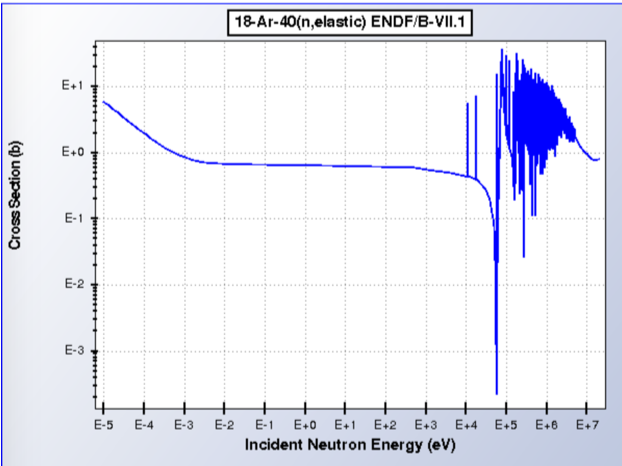
\includegraphics[width=0.4\linewidth]{Figures/Ar40xsec.png}
%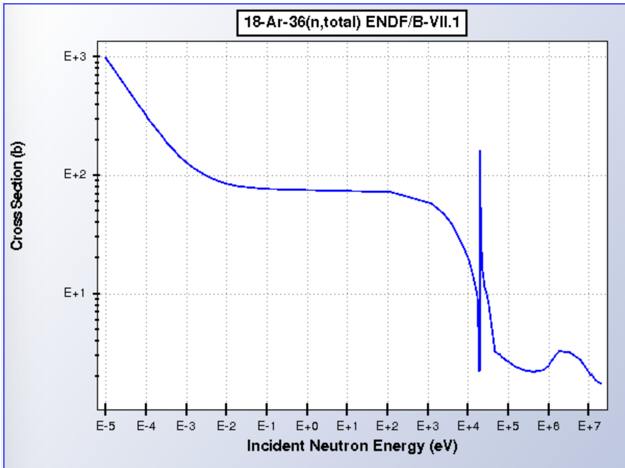
\includegraphics[width=0.4\linewidth]{Figures/Ar36xsec.png}
%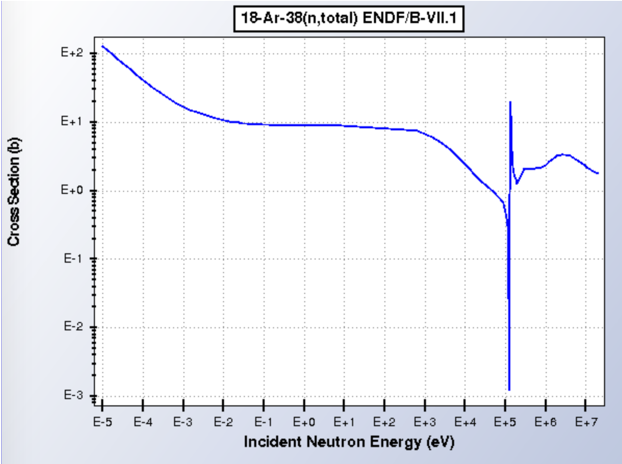
\includegraphics[width=0.4\linewidth]{Figures/Ar38xsec.png}
%\caption{Elastic scattering cross sections on 40-Ar (top left), 36-Ar (top right), and 38-Ar (bottom). From ENDF/B-VII.1~\cite{ref:ENDF}. The large anti-resonance at $57\; keV$ in 40-Ar can be clearly seen.
%{\bf NOTE: PUT IN PLOTS FOR ELASTIC}
%}
%\label{fig:Arxsec}
%\end{center}
%\end{figure}


%\begin{figure}[h]
%\begin{center}
%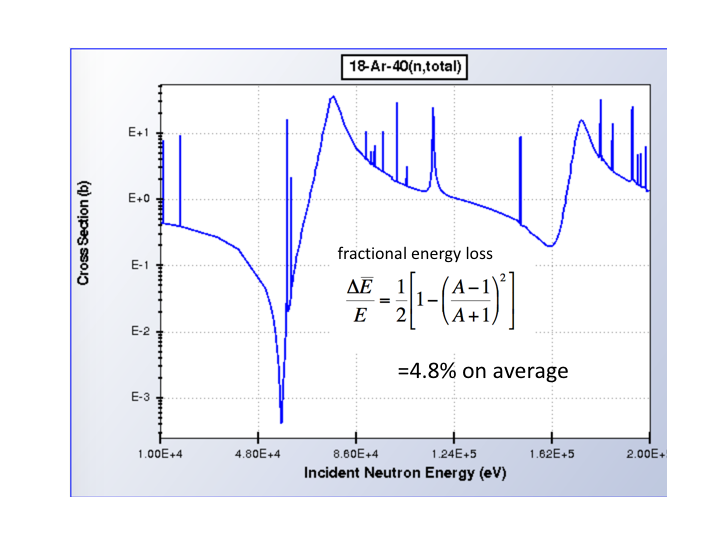
\includegraphics[width=0.75\linewidth]{Figures/Ar40Xsec2.png}
%\caption{Total scattering cross sections on 40-Ar in the range $10-200\; keV$~\cite{ref:ENDF}}
%\label{fig:Arxsec2}
%\end{center}
%\end{figure}

Liquid argon is near transparent to neutrons with an energy near or at 57~keV due to an anti-resonance in the cross-section caused by the destructive interference between two high level states of the $^{40}$Ar nucleus. The cross-section at the anti-resonance ``dip" is about 10~keV wide, and at the bottom the cross section of $1.6\times 10^{-4}\;$b implies an elastic scattering length of over $2,000\;$m. %Of course, natural 
Natural argon has three major isotopes: 36-Ar (0.3336\%), 38-Ar (0.0834\%), and 40-Ar (99.6035\%) each with a slightly different anti-resonance. The average elastic scattering length of the 57~keV neutrons in natural liquid argon is about $30\;$m.

The neutrons at the anti-resonance energy could be injected into liquid argon TPC, provided no material (e.g. hydrocarbons) blocks the path. Those that do scatter lose energy, leave the anti-resonance, quickly slow down and are captured. Each capture releases exactly the binding energy difference between $^{40}$Ar and $^{41}$Ar, about $6.1\; MeV$ in the form of $\gamma$ rays.  As will be described below, by using a {\it DD} Generator (where {\it DD} stands for "Deuterium-Deuterium"), a triggered pulse of neutrons can be generated outside the TPC, then injected via a dedicated hole in the insulation into the liquid argon, where it spreads through the 58~m volume of the detector to produce $6.1\; MeV$ energy depositions.
%Using this method, the calibration procedure would be quick (likely a few hours depending on the neutron yield of the DD generator), and there is no need to manufacture short-lived isotopes at an external facility.

The neutron capture $\gamma$ spectrum has been measured and characterized. Recently, the ACED Collaboration performed a neutron capture experiment using  the Detector  for Advanced  Neutron  Capture  Experiments  (DANCE)  at the  Los  Alamos  Neutron  Science  Center  (LANSCE). The result was published~\cite{aced} and will be used to prepare a database for the neutron capture studies.

%{\it Mention Test at LANSCE and its role?}

%%%%%%%%%%%%%%%%%%%%%%%%%%%%
\subsubsection{Design}
\label{sec:sp-calib-sys-pns-des}

The basic design concept of such a pulsed neutron source has been used successfully for Boron Neutron Capture Therapy\cite{KOIVUNORO2004853}. The design of the Pulsed Neutron Source used for energy calibration is shown in Figure~\ref{fig:PNS_Moderator}. The system will consist of four main components: a $DD$ generator, an energy moderator reducing the energy of the $DD$ neutrons down to the desired level, and the shielding materials, and a neutron monitor to confirm neutron flux and safe operation. 

\begin{figure}[tpb]
\centering
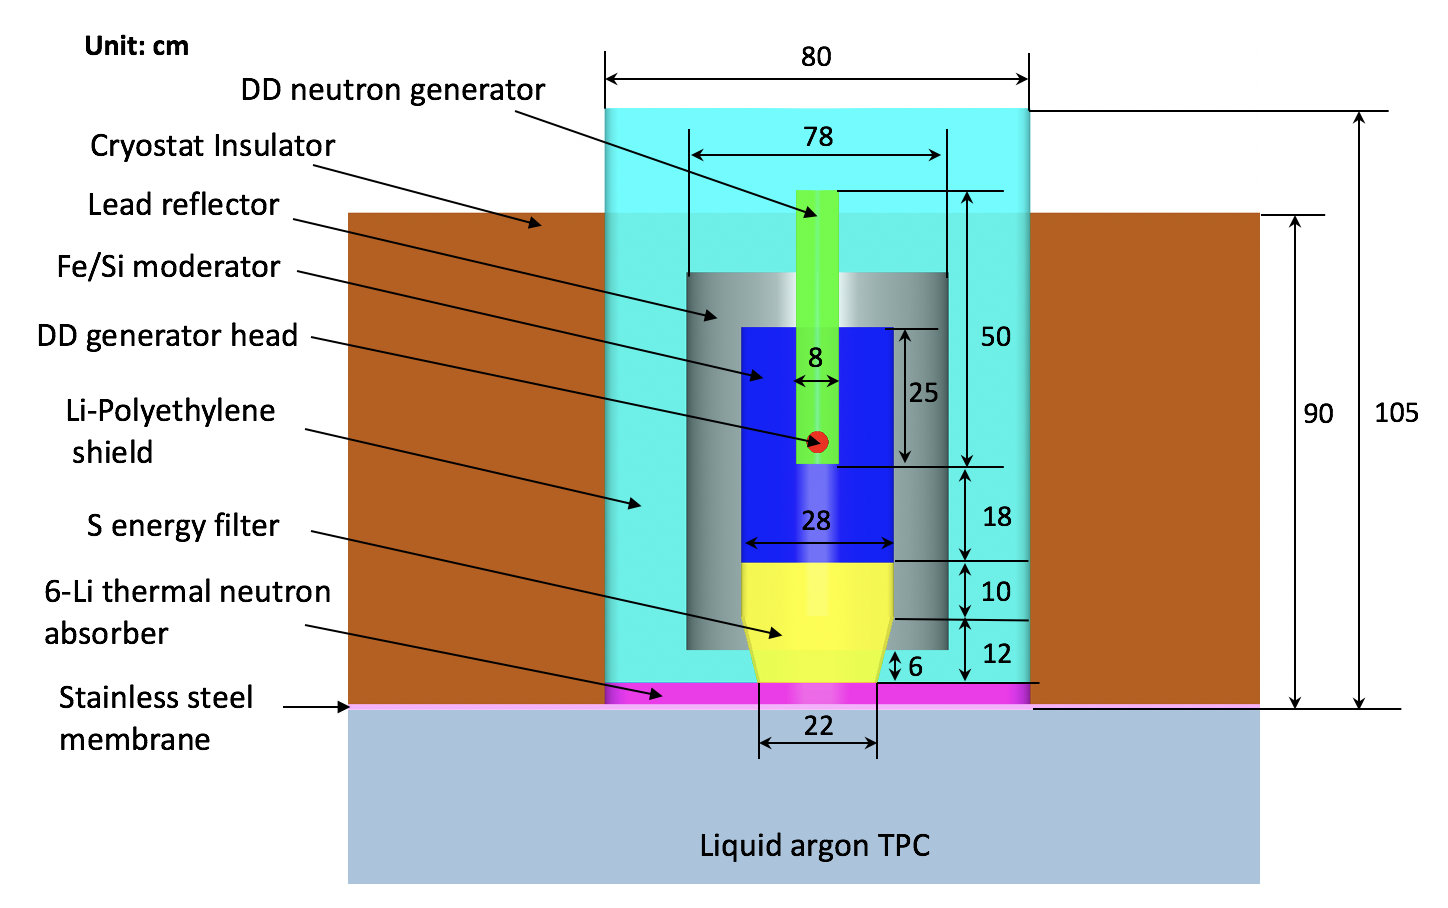
\includegraphics[width=12cm]{graphics/PNS_Moderator.png}
\caption{Conceptual design of the Pulsed Neutron Source. The whole device is placed outside the TPC volume on top of the cryostat.}
\label{fig:PNS_Moderator}
\end{figure}

{\bf DD generator source:} $DD$ generators are commercial devices that can be readily obtained from several vendors at a cost of about \$~125k each, which includes all control electronics. The pulse width is adjustable and can be delivered from about 10-1000~$\mu$s (which affects the total output). 

{\bf Moderator:}  A feasible moderator has been designed using a layered Moderator (Fe or Si)-Filter(S)-Absorber(Li) %layered 
configuration. The 2.5~MeV neutrons from the $DD$ generator are slowed down to below 1~MeV by the energy moderator. Natural iron and silicon are found to be efficient moderators for this purpose. Then an energy filter made of sulfur powder is used to further select the neutrons with desired anti-resonance energy.
The neutron anti-resonance energy in $^{32}$S is 73~keV, right above the 57~keV anti-resonance energy in $^{40}$Ar. The neutrons at this energy lose about 3.0~keV per elastic scattering length. After a few elastic scattering interactions, most of the 73~keV neutrons selected by the sulfur filter will fall into the 57~keV anti-resonance energy region in liquid argon. These materials require no cooling or special handling. Finally, a thermal absorbing volume of Lithium is placed at the entry to the argon pool in order to capture any neutrons that may have fallen below the 57~keV threshold. The reflecting volume is added around the $DD$ generator and the neutron moderator to increase downward neutron flux. 

{\bf Shielding:} The source will be encased in a shielding volume. The goal of the shield is to block both scattered neutrons and gammas which are produced in the source. Lithium-Polyethylene (7.5~$\%$) is chosen to be the material for the neutron shield because it is rich in hydrogen and lithium atoms which yield a high neutron absorption cross section. Lithium-Polyethylene is also light weight, commercially available, and relatively inexpensive. The energy spectrum entering the shield has multiple peaks between 0.5~MeV and 1.5~MeV, and one major spike at 2.2~MeV. The shield is able to effectively block the lower energy peaks but is only able to degrade the intensity of the 2.2~MeV peak. This is because 2.2~MeV gammas are a characteristic signature for neutron captures on hydrogen. A safe thickness of the lithium-polyethylene shield must be found such that it is capable of degrading the dose of 2.2~MeV gammas to safe levels. The dose of radiation from 2.2 MeV gammas was then calculated assuming a person standing 1~m away. Simulation indicates that 12~cm of Lithium-Polyethylene shield satisfies basic safety requirements. 

{\bf Neutron Monitor:} The system will need a monitoring system to confirm the source is operating as expected.  A neutron monitoring detector consisting of an Eljen EJ-420 coupled to an ADIT L51B16S 2-inch PMT will be placed just outside of the moderating material surrounding the $DD$ generator and will be read out with a CAEN waveform digitizer with neutron/$\gamma$ pulse-shape discriminating firmware. The monitoring detector will provide relative flux information to the calibration users and will ensure that the intensity of the source is constant, thereby allowing a comparison of data taking at different times.  A small collimator will be placed in front of the neutron detector, and inside the shielding material of the $DD$ source. The collimator dimensions and material specifications (likely a combination of iron, lead, and polyethylene) will be optimized from Monte Carlo simulations.

Based on the general concept, two different designs were studied with GEANT4 simulation. Figure~\ref{fig:PNS_source_design} shows a conceptual layout of the neutron injection system. %\todo{For v2, confirm updated figure; minor error in current one.}

\begin{figure}[tpb]
\centering
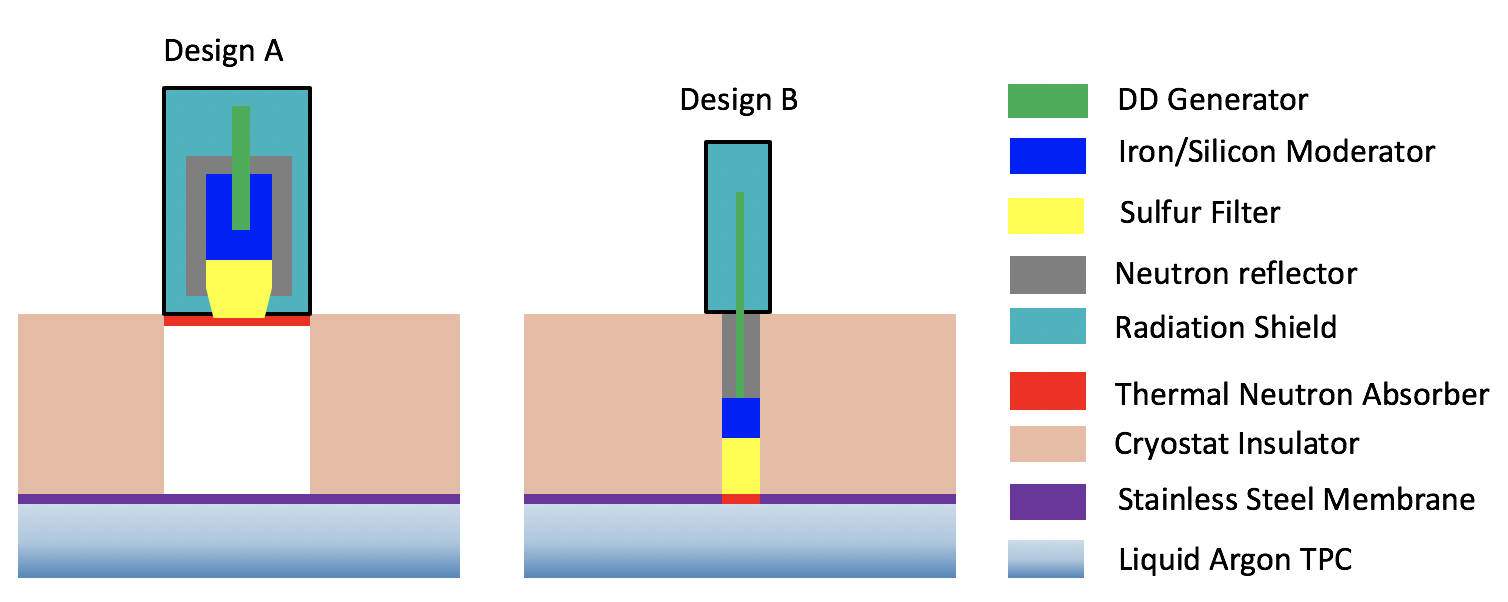
\includegraphics[width=16cm]{graphics/PNS_Two_Designs.png}
\caption{Two designs currently under development for the Pulsed Neutron Source. Design A: Large format neutron source to be deployed above/inside the human access holes or other delicate neutron injection ports; Design B: Small format neutron source to be deployed inside the calibration feedthrough ports.
%, see text for more details.
}
\label{fig:PNS_source_design}
\end{figure}

\begin{itemize}
\item Design A: Large format Moderator; \\
The neutron source is about 0.8~m wide and 1~m high. It would sit above the cryostat insulator. Beneath the neutron source, a cylinder insulator volume with a diameter of more than 50~cm has to be removed to allow the neutrons to get into the cryostat. Such an interface is provided by the human access ports near the endwalls of the detector; a picture of this is shown for \dword{protodune} in Figure~\ref{fig:humanaccessport}. The top flange is sealed, and the neutron source sits on top (Design A), providing heat insulation; The neutron source weighs about 1.6~tons and will hang on the I-beam supporting structure. This design allows a permanent deployment of the neutron source. GEANT4 simulation has shown that 0.13 ~\% of the neutrons generated by the $DD$ generator are expected to be captured inside the liquid argon TPC. It is also possible to place the neutron source inside the human access port which would allow a factor of 6 increase of the neutron flux but require a modification of the interface flange. This is currently being investigated.
% JW: I think It doesn't harm to mention that the neutron source could be placed inside the manhole. My recent simulation is based on this configuration.

%\item \fixme{KM: I do not think this is possible for quite a few reasons-- heat loss and also cost of adjusting this. Remnoving this for now.} Design B: Large format Moderator; no insulation between Moderator and cryostat membrane The design of the the neutron source itself would be same as Design A. The only difference is that the neutron source will be placed inside a hole on the cryostat insulator. The cryostat will be kept closed, but there is no vacuum insulation between the neutron moderator and the stainless steel membrane. As the neutron source is closer to the liquid argon cryostat, the neutron flux is expected to be a factor of 10 higher than that of Design A. However, the neutron source must be removed and the insulator has to be recovered after the calibration run. 
\item Design B: Small format Moderator; no insulation between Moderator liquid argon. An alternative method for delivering the neutrons is to use the existing calibration feedthroughs. In the current cryostat design, 20 calibration feedthroughs with a 20~cm inner diameter will be available on top of the cryostat. One can design the neutron source with an ultra-thin $DD$ generator that fits the size of the feedthrough. The problem is that there will be no space in the feedthrough for the shielding materials to fit in, so additional shielding will need to be placed around the feedthrough. The weight of this compact neutron source will be about 140~kg, so mounting will be simpler compared to Design A. The effective neutron flux is expected to be similar as that of Design A. 
\end{itemize}

\begin{figure}[tpb]
\centering
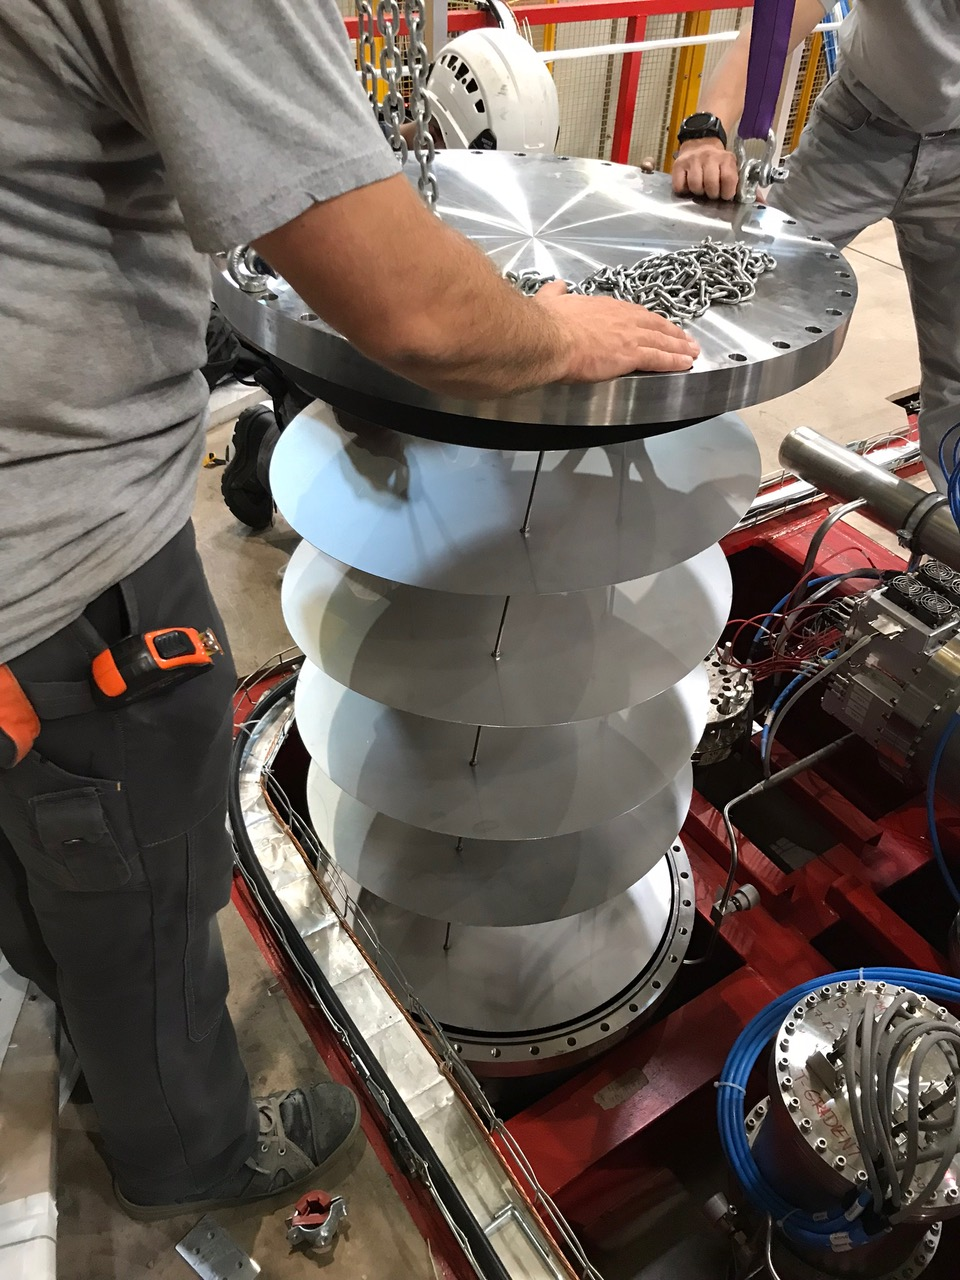
\includegraphics[width=6cm]{graphics/manhole2.jpg}
\caption{Flange for human access port on ProtoDUNE-SP and support structure (red frame).}
\label{fig:humanaccessport}
\end{figure} 

\begin{figure}[tpb]
\centering
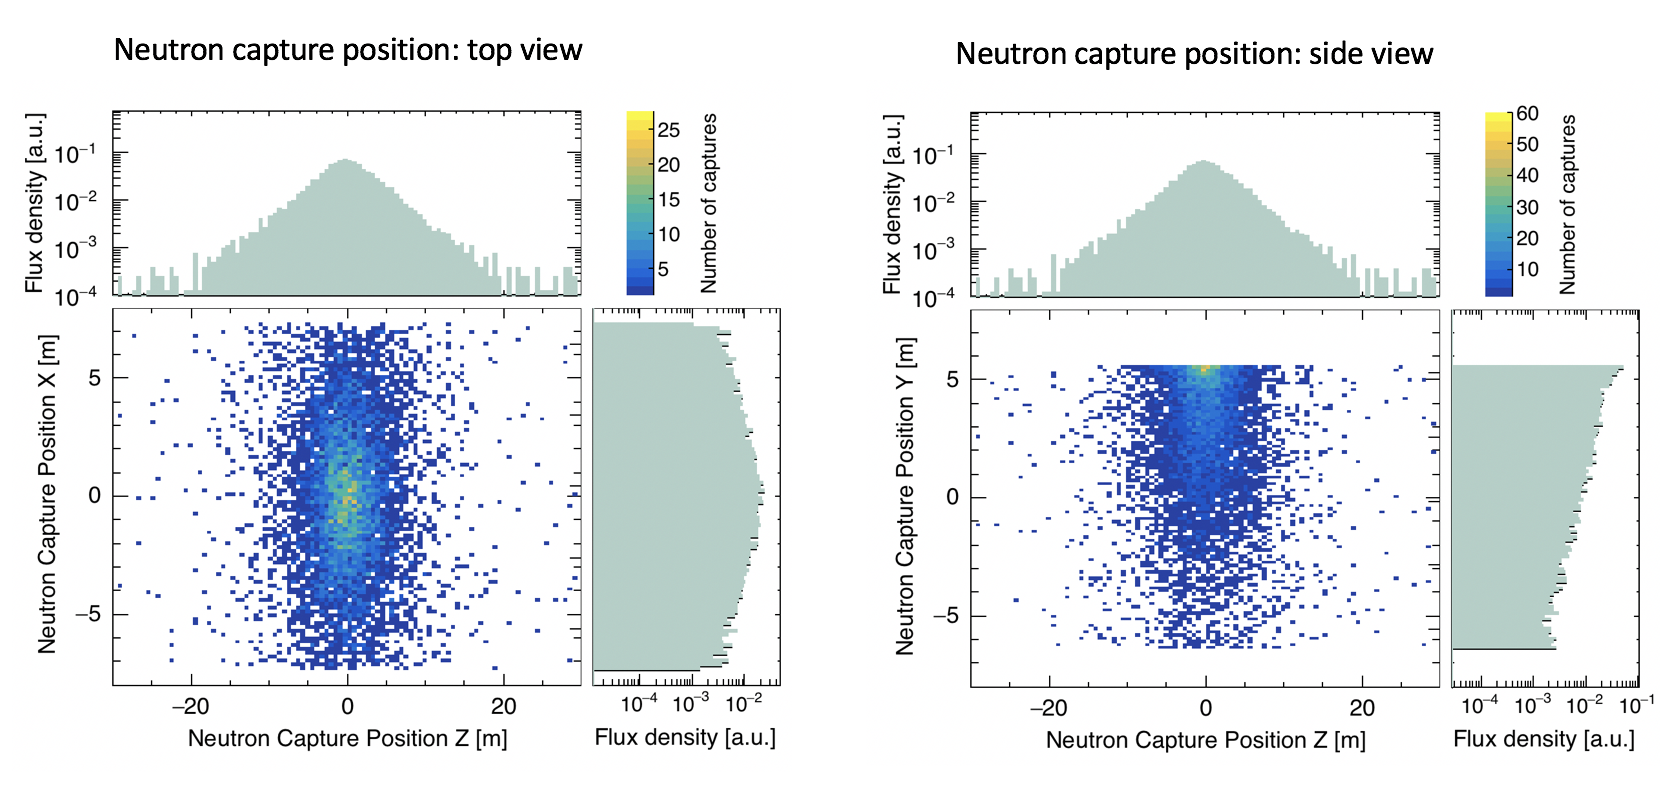
\includegraphics[width=18cm]{graphics/PNS_NcapPosition.png}
%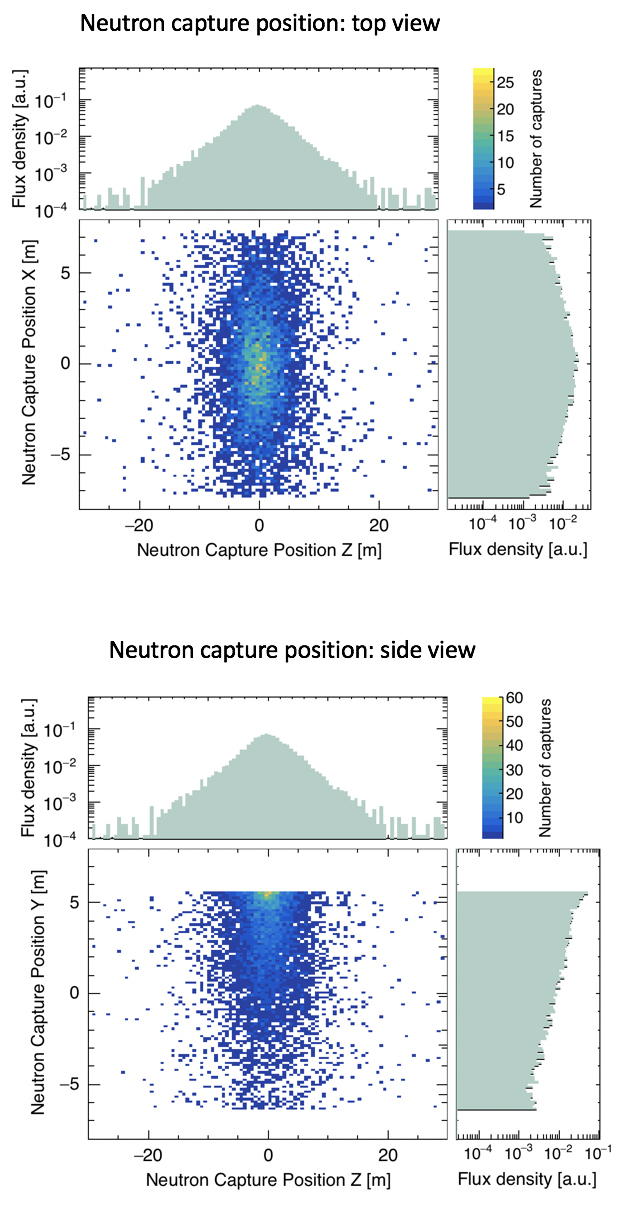
\includegraphics[width=10cm]{graphics/PNS_NcapPosition_v2.png}
\caption{Neutron capture positions inside a DUNE sized TPC. L=60~m (along Z axis, horizontally parallel to the beam direction), W=14.5~m (along X axis, horizontally perpendicular to the beam direction), H=10~m (along Y axis, vertically perpendicular to the beam direction). The neutron moderator is based on Design A, but the entire source is placed inside the injection port that is central to the cryostat. 10$^{6}$ DD generator neutrons with 2.5~MeV energy were simulated in the moderator and propagated inside the liquid argon TPC. Left: Top view of neutron capture positions. Right: Side view of neutron capture positions.} 
\label{fig:ncapposition}
\end{figure} 

The two designs were simulated in GEANT4. The position distribution of the neutron captures is shown in Fig.~\ref{fig:ncapposition}. In the simulation, the Pulsed Neutron Source is placed on top of the liquid argon cryostat with the same size as the DUNE 10~kton TPC. Initial simulation results indicate that one Pulsed Neutron Source could cover half the TPC volume, so two identical neutron sources, each central to half the cryostat top,  %\todo{SG: I assume this is with design A, right? if so, mention which design}
would illuminate the whole TPC volume of the DUNE far detector for both designs. However, this would require opening two additional neutron injection ports which are not included in the current cryostat design \footnote{Ideally,opening two identical neutron injection ports for each 10~kton TPC would make full use of the neutron source. The possibility requires further discussion with the cryostat engineers.}. Alternatively, two large format neutron sources (Design A) could be permanently deployed at the human access holes at the corners of the cryostat. One concern is that the neutrons scattered from the liquid argon volume from the human access holes may not reach the center of the TPC. This can be mitigated by using a small format neutron source (Design B) deployed on top at the center of the cryostat using the multi-purpose feedthroughs. %could be used to complement the coverage of the large format sources. 
Figure~\ref{fig:PNS_energy_design} shows the energy spectrum of the neutrons moderated and injected to the liquid argon TPC, based on Design A.
% This figure is based on Design A moderator placed inside the manhole. We can still use this figure, because the energy spectrum shape should be same. Only the flux will be a factor of 6 lower
%The neutron energy is moderated from 2.5 MeV to below 100 keV.  

\begin{figure}[tpb]
\centering
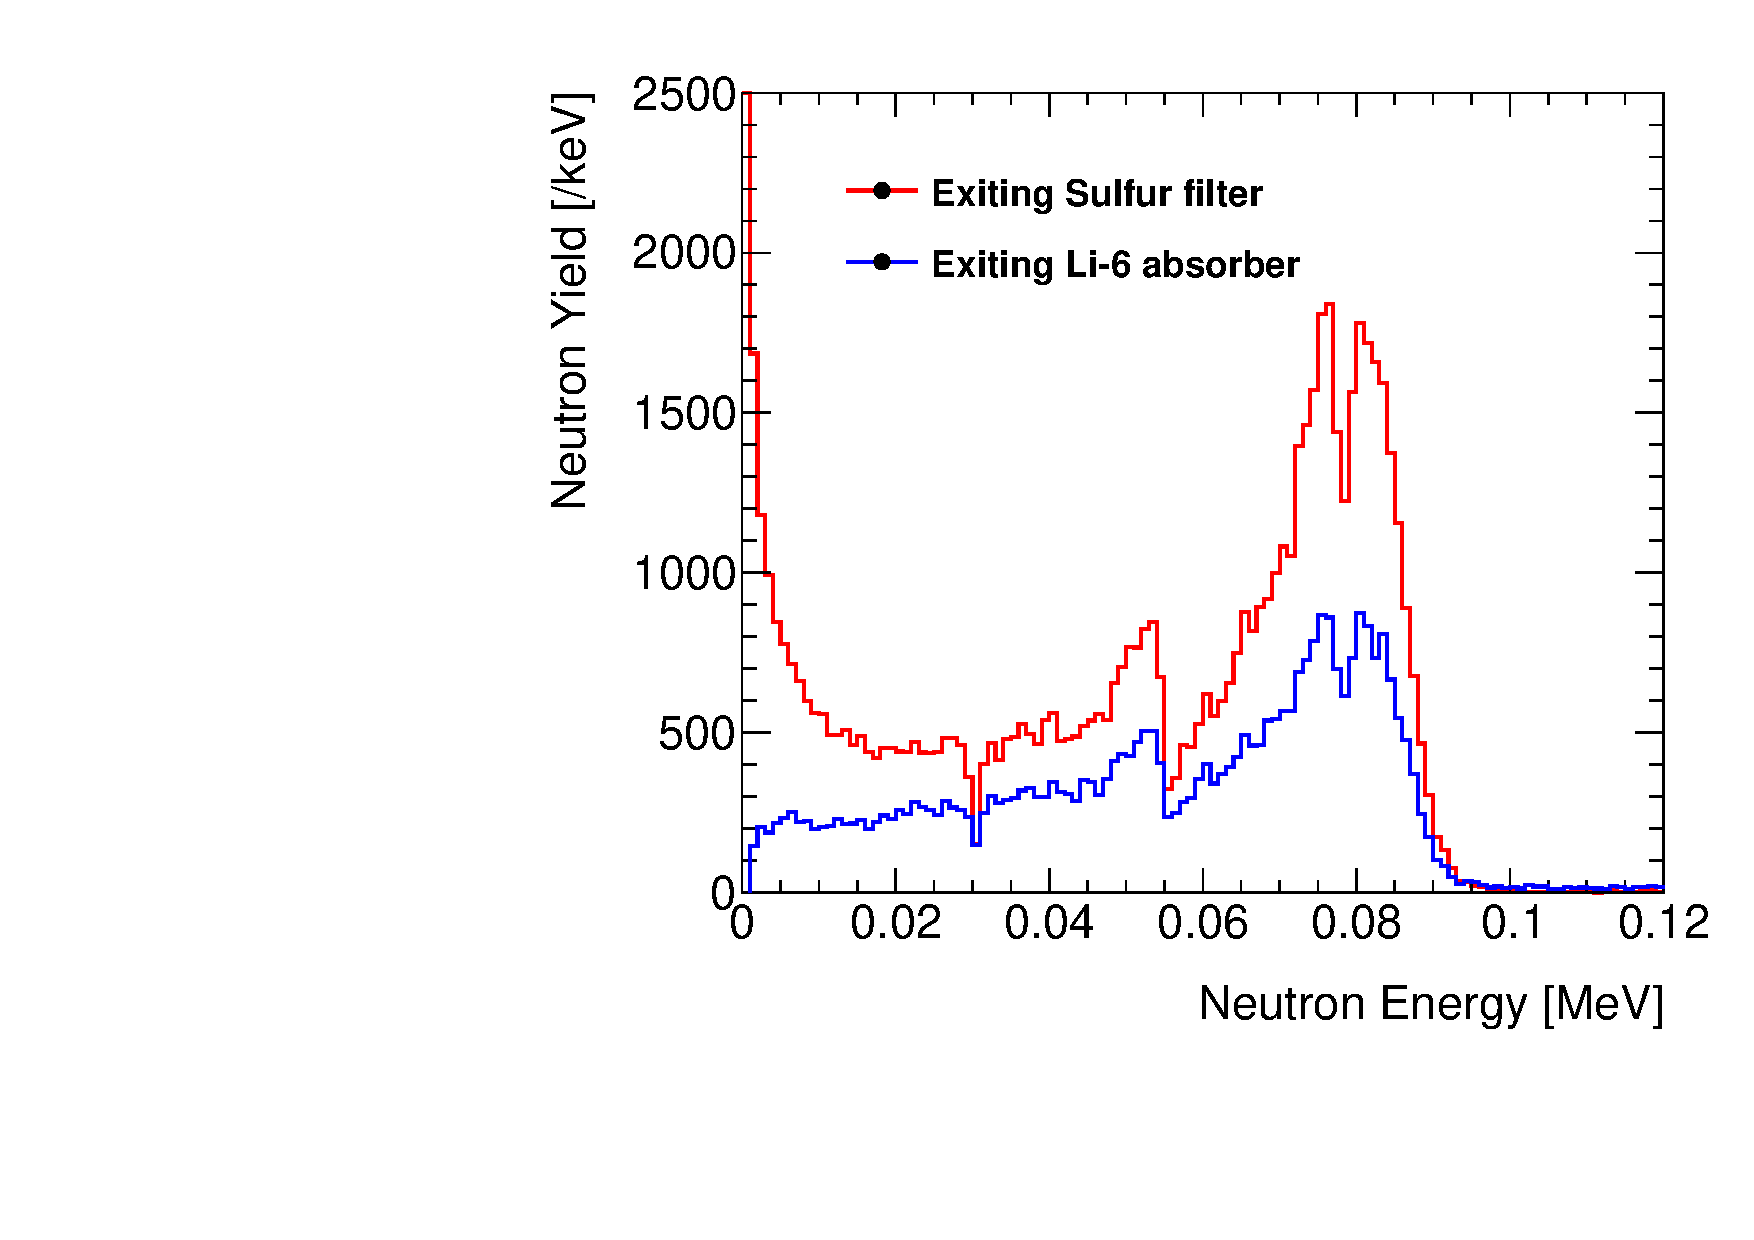
\includegraphics[width=10cm]{graphics/PNS_Energy_Moderator.pdf}
\caption{Energy of moderated neutrons produced by the Pulsed Neutron Source. Simulation is based on Design A. The total number of initial DD generator neutrons is 10$^{6}$ }
\label{fig:PNS_energy_design}
\end{figure} 

The system is expected to have a long lifetime of operation, but as the PNS system sits on top of the cryostat, with no opening to the liquid argon, it is possible to replace the system if it fails with only crane support.


%%%%%%%%%%%%%%%%%%%%%%%%%%%%
\subsubsection{Possible Measurements}
\label{sec:sp-calib-sys-pns-meas}

The 6.1~MeV $\gamma$ cascade will provide a uniform signal for neutron capture, part of the supernova signal. The source may also be used determine the relative efficiency across the detector for neutron capture, and also provide measurements of energy resolution and energy scale spatially and temporally resolved. Simulation studies are currently underway and for the second draft, we plan to include a first round of simulation results.

%\todo{Simulation studies are underway but changing rapidly. for v2 we will include a first round of studies.}







%%%%%%%%%%%%%%%%%%%%%%%%%%%%%%%%%%%%%%%%%%%%%%%%%%%%%%%

\subsection{Proposed System: Radioactive Source Calibration System}
\label{sec:sp-calib-sys-rs}

% \fixme{Call it "deployment" or "calibration" system?}
%%%%%%%%%%%%%%%%%%%%%%%%%%%%%%%

%\fixme{KM: done for now, but am not satisfied with the end of it-- Juergen did not provide measurements! SG/JM: please briefly check to make sure it is coherent? SG: done. Sent an email to Juergen with some items to be addressed.}

%\subsubsection{Physics Motivation}

Radioactive source deployment provides an in-situ source of physics signals at a known location and with a known activity that can be chosen such that there is only one calibration event per drift time window. The baseline source design probes de-excitation products (gamma-rays) which are directly relevant for detection of supernova neutrinos and $^{8}B$/hep solar neutrinos. The \dlong{rsds} (\dshort{rsds}) is the only calibration system that could probe the detection capability for single isolated solar neutrino events and study how well radiological backgrounds can be suppressed. The trigger efficiency could be studied %versus 
as a function of threshold. 

Secondary measurements from the baseline source deployment include electro-magnetic (EM) shower characterization for long-baseline $\nu_e$ CC events, electron lifetime and electric field as a function of \dword{detmodule} vertical position, individual light detector response, and determination of radiative components of the Michel electron energy spectrum from muon decays. Aside from the baseline $^{58}$Ni(n,$\gamma$)$^{59}$Ni 9 MeV gamma-ray source, other sources could be deployed with the same multi-purpose system, for example a $^{40}$Ar($\alpha,\,\gamma$)$^{44}$Ca gamma-ray source, a $^{252}$Cf and/or AmBe neutron source that probe the impact of various radiological backgrounds, like radon ($\alpha,\,\gamma$) or radiological neutrons, or simply measure the neutron tagging efficiency, useful for improved calorimetry of beam neutrino interactions. In contrast to the baseline $^{58}$Ni(n,$\gamma$)$^{59}$Ni source with 9 MeV gamma-rays, a $^{40}Ar(\alpha,\,\gamma)^{44}$Ca source producing gamma-ray energies around 15~MeV could even be deployed outside of the cryostat and probing the upper visible energy range and trigger efficiency for $^{8}B$/hep solar neutrinos. 

Both the \dshort{rsds} and the pulsed neutron source system are needed to address the integrated response of the detector for low energy physics. 
The \dword{rsds} primarily probes for trigger efficiency, the \dword{pns} tests mostly for uniformity. Response in Ar may change rapidly as a function of photon energy due to underlying nuclear physics mechanisms. A combination of 6~MeV (direct neutron capture response), 9~MeV (peak visible $\gamma$-energy of interest to \dword{snb} and $^{8}B$/hep solar neutrinos), 15~MeV (upper visible energy of $^{8}B$/hep solar neutrinos) and decay electrons ($\sim$30~MeV) is needed to map the low energy response. In terms of complementarity, radioactive sources provide a known position, known-energy single photon events that could be triggered on, while the pulsed neutron source provides a simple, potentially, non-invasive design with externally triggered multi-photon energy signature which is visible across the entire detector with a known time signature.


%%%%%%%%%%%%%%%%
\subsubsection{Design Considerations}

A composite source can be used that consists  of $^{252}$Cf, a strong neutron emitter, and $^{58}$Ni, which, via the $^{58}$Ni(n,$\gamma$)$^{59}$Ni process, converts one of the $^{252}$Cf fission neutrons, suitably moderated, to a monoenergetic \SI{9}{\MeV} photon~\cite{Rogers:1996ks}. 
The source is envisaged to be inside a cylindrical moderator with mass of about \SI{15}{kg} and a diameter of \SI{20}{\cm} such that it can be deployed via the multipurpose instrumentation ports discussed in Section~\ref{sec:calib-ports}. The activity of the radioactive source is chosen such that no more than one \SI{9}{\MeV} capture $\gamma$-event occurs during a single drift period. This forms the main requirement for this system as this allows one to use the arrival time of the measured light as a $t0$ and then measure the average drift time of the corresponding charge signal(s). Table~\ref{tab:fdgen-calib-all-reqs-rsds} lists the full set of requirements for the \dlong{rsds}.

The sources would be deployed outside the \dword{fc} within the cryostat to avoid regions with a high electric field, about \SI{30}{\cm} from the field cage. The $\gamma$-ray would need to travel about two attenuation lengths (including the \SI{10}{\cm} radius of the source body). Such high $\gamma$-energies are typically only achieved by thermal neutron capture, which invokes a neutron source surrounded by a large
amount of moderator, thus making such an externally deployed (n, $\gamma$) source \SI{20}{\cm}  to \SI{50}{\cm} % large
in diameter. 

\begin{dunetable}
[Full specifications for the radioactive source deployment system]
{p{0.45\linewidth}p{0.25\linewidth}p{0.25\linewidth}}
{tab:fdgen-calib-all-reqs-rsds}
{Full list of Specifications for radioactive source deployment system.}   
Quantity/Parameter	& Specification	& Goal		 \\ \toprowrule   
%\textbf{Proposed Radioactive Source System}	   &   &  \\ \colhline  
Distance of the source from the field cage & 30 cm & \\ \colhline
Rate of 9~MeV capture $\gamma$-events inside the source {(\it top-level requirement)} & < 1kHz & \\ \colhline 
Data volume per 10~kton & 50~TB/year & 100~TB/year \\ \colhline 
Longevity	& \dunelifetime			& > \dunelifetime   \\ \colhline    
%Stability & Match precision requirement at all places/times	&  \\ \colhline  Reliability	& Measurements as needed & Measurements as needed \\ \colhline

\end{dunetable}

In~\cite{Rogers:1996ks}, %\fixme{This needs to be restated: In Jones [4]... (with Jones being the name of the author).}
%\cite{Triumf:Nickelsource} 
%\todo{SG: reference needs fixing},
a $^{58}$Ni (n,$\gamma$) source, triggered by an AmBe neutron source,
has been successfully built, yielding high $\gamma$-energies of \SI{9}{\MeV}. DUNE %We
proposes to use a $^{252}$Cf (or AmLi as backup) neutron source with lower
neutron energies, which requires less than half of the surrounding
moderator, and making the $^{58}$Ni (n, $\gamma$) source only
\SI{20}{\cm} or less in diameter. The multipurpose instrumentation
feedthroughs at either end of the cryostat are sufficient for
this, and have an inner diameter of \SI{25}{\cm}.  The moderator
material chosen for DUNE is Delrin,\footnote{DuPont\texttrademark Delrin\textregistered, \url{http://www.dupont.com/products-and-services/plastics-polymers-resins/thermoplastics/brands/delrin-acetal-resin.html}.} which has a large enough
density to avoid flotation. Further, the end caps of the source
body are round to avoid distorting the electric field and to
eliminate the risk of the source getting stuck during deployment. 
Figure~\ref{fig:RadioactiveSource_zm40cm_xp220cm} depicts the baseline source design of a
cylindrical Delrin moderator with a diameter of \SI{20}{\cm}, a
height of \SI{40}{\cm} including half-spheres at either end with
radius of \SI{10}{\cm}, deployed at $z$=\SI{40}{\cm} leaving a gap of \SI{30}{\cm} towards the \dword{fc} and at a distance to the \dword{apa} of $x$=\SI{220}{\cm}, 
which is slightly further than mid-drift.

\begin{dunefigure}[Fish-line deployment scheme in DUNE for an encapsulated radioactive source]{fig:RadioactiveSource_zm40cm_xp220cm}{Fish-line deployment scheme in DUNE for a radioactive source encapsulated inside a cylindrical Delrin moderator body \SI{20}{\cm} in diameter and \SI{40}{\cm} high, including half-spheres with a radius of \SI{10}{\cm} at either end. A $^{252}$Cf neutron source and a natural Ni target are sealed inside at the center. The fish-line is deployed \SI{40}{\cm} outside of the \dword{fc} and \SI{220}{\cm} away from the \dword{apa} (red plane).}
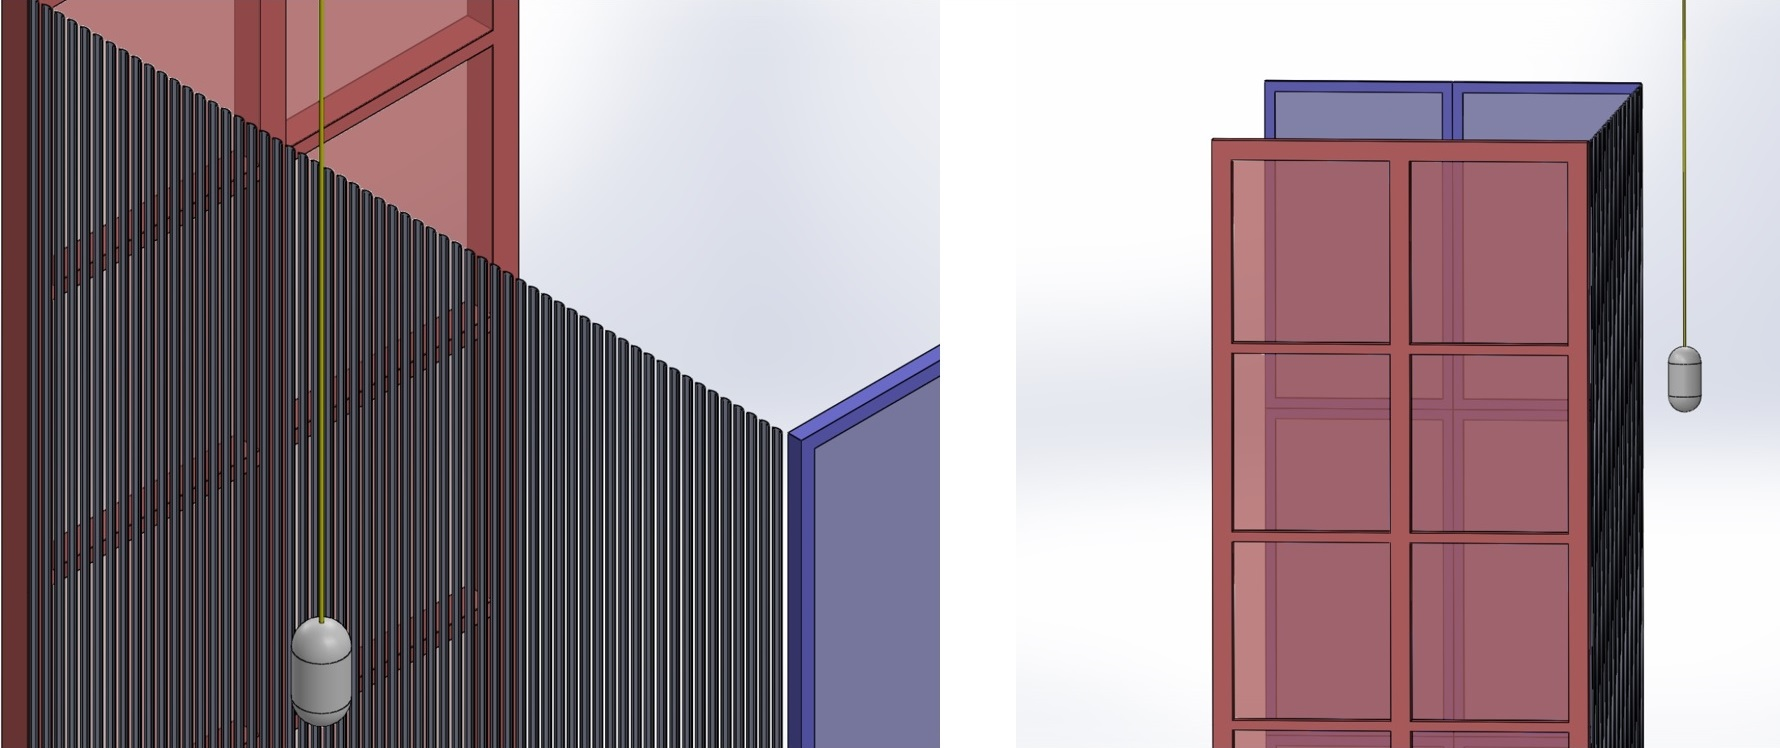
\includegraphics[width=1.0\linewidth]{RadioactiveSource_zm40cm_xp220cm.jpg}
\end{dunefigure}

% Here it is, but I don't have privileges for the bibliography

%@Misc{Triumf:Nickelsource,
%  author =   {J. Rogers, M. Andreaco, C. Moisan},
%  title =    {A $7-9$\,MeV isotropic gamma ray source for detector testing},
%  howpublished = {TRIUMF TRI-PP-96-7},
%  month =    {Apr},
%  year =     {1996},
%}

%\fixme{KM: From Juergen but I think covered by above: The activity of the radioactive source is chosen such that no more than one \SI{9}{\MeV} capture $\gamma$-ray spills into the active \dword{lartpc} region during a single \SI{2.2}{\milli\s} drift period. This allows one to use the arrival time of the measured light as $t_{0}$ and then measure the average drift time of the corresponding charge signal(s). The resulting drift velocity in turn yields the electric field strength, averaged over the variations encountered during the drifting of the charge(s). This can be repeated for each single \SI{9}{\MeV} capture $\gamma$-event that occurs during a \SI{2.2}{\milli\s} drift period and where visible $\gamma$-energy is deposited inside the active volume of the TPC. Pile-up and data read-out considerations restrict the maximally permissible event rate to less than \SI{10}{\hertz} and in turn the \SI{9}{\MeV} capture $\gamma$-rate occurring inside the radioactive source body to less than \SI{140}{\hertz}, given a spill-in efficiency into the active \dword{lar} of about \num{7}\%.}

A successfully employed multipurpose fish-line calibration
system
%~\cite{bib:deKerret2012} \todo{SG: Juergen to provide proper reference. JM: Juergen says there's no alternative public ref.} 
% JM, April 2018: We will not refer to this since the LBNC will not have access to it
%\fixme{need to add reference: "The Double Chooz Near Detector Technical Design Report" 
%Double Chooz Collaboration (H. de Kerret (APC, Paris) et al.) Oct 1, 2012. EDMS ID:I-028812 ; DocDB ID: 3403-V5 Pages 198 - 223
%(Anne can't find proper ref for this)}
 for the Double Chooz
reactor neutrino experiment has become available for DUNE after
the decommissioning of Double Chooz in 2018. The system can be
easily refitted for use in DUNE. The system will be housed inside
a purge-box that is connected via a neck to a multipurpose
calibration feedthrough with a closed gate valve on top of the
cryostat. Before deployments, the source will be gently cooled-down by blowing liquid argon boil-off onto it inside a sealed purge-box. After the source has reached 
%near liquid argon 
near-\dword{lar} temperatures, the purge-box will be evacuated by a vacuum pump to remove any residual oxygen and nitrogen which is monitored at the ppm level. Then, the entire purge-box interior is purged with boil-off liquid argon, and the pressure equalized with the gas pressure inside the detector, before the gate-valve is opened and deployments can commence. This procedure ensures that no significant impurities are introduced into the detector during a deployment and that no significant amount of liquid argon is boiled-off from the detector. 
%Also, if the source is in close proximity of an \dword{apa} wire frame, lower energetic radiological backgrounds become problematic as the source light and charge yield is reduced exponentially with distance. 

Deployed near mid-drift (in each TPC module) the \SI{9}{\MeV}
$\gamma$-ray source can illuminate the full drift length from
\dword{apa} to \dword{cpa}. The sources are retrieved from the
detector after each deployment and stored outside the cryostat following approved safety protocols, and the gate-valves are kept closed after deployments. More details on radiation safety and handling procedures are presented in Section~\ref{sec:sp-calib-rsds-safety}.

\subsubsection{Development Plan}
The major development plans for the \dlong{rsds} include
\begin{itemize}
\item Continued development of relevant simulation tools including geometry representation of the source deployment system and impact from various radiological contaminants on detector response. 
\item Studies to suppress radiological backgrounds for the calibration source.
\item Simulation studies to understand data and trigger rates.
\item A baseline design source with Delrin moderator, $^{252}$Cf neutron source, and natural nickel target, both sealed inside at the moderator's center.
\item Validation of \SI{9}{\MeV} capture $\gamma$-ray yield of source using spectroscopic measurements with the `RABBIT' germanium detector at the South Dakota School of Mines and Technology, that has an assay chamber large enough to fit the bulky moderator. 
%\fixme{Check this please. SG: check what?}
\item Validation with $^{3}$He based hodoscope at South Dakota School of Mines and Technology to ensure that the flux of neutrons escaping the moderator is not an issue; otherwise use lower energetic AmLi neutron source instead and/or more moderator material, and/or different geometric configuration of nickel target. 
\item Test gentle GAr cooling of source and validate material integrity. Measure tensile strength of braided SS-304 wire-rope at cryogenic temperatures and ensure a safety factor of one order of magnitude by adjusting number of steel braids and their diameters. Validate cryogenic shrinkage of sectional teflon sleeves, that enclose the braided steel wire-rope and electrically insulate it towards the \dword{fc}. 
\item Validation that anticipated fluid flow in \dword{lar} does not cause oscillations of the source; otherwise design vertical guide wires to be pre-installed during detector installation 
%and that they 
which will keep source in stable position during deployment along the vertical axis.
%\item A mechanical test of the Double Chooz fish-line deployment system with both an \dword{lar} and liquid nitrogen mock-up column in the high bay lab at South Dakota School of Mines and Technology. The ultimate test of the system will be done at ProtoDUNE. 
\item Explore other radioactive sources beyond the baseline $^{58}$Ni(n,$\gamma$)$^{59}$Ni 9 MeV gamma-ray source, for example a non-invasive externally employed $^{40}$Ar($\alpha,\,\gamma$)$^{44}$Ca 15~MeV gamma-ray source with $^{241}$Am that is currently being assembled at SDSMT, and that could probe from the outside of the cryostat the upper visible energy range and trigger efficiency for $^{8}B$/hep solar neutrinos. Furthermore, investigate hybrid neutron sources ($^{252}$Cf and AmBe) that emulate the kinetic neutron energy spectrum of radiological neutrons and probe the neutron tagging efficiency, useful for improved calorimetry of beam neutrino interactions and for clarification of impact of radiological neutron backgrounds. 
\end{itemize}

A successful demonstration of the \dword{rsds} in \dword{protodune2} running is the main priority for this system towards making a decision on deploying this system for the \dword{fd}. A schedule with main steps towards \dword{protodune2} deployment is shown in Table~\ref{tab:calib-rsds-sched}.

\begin{dunetable}
[Key Milestones for Commissioning RSDS in ProtoDUNE-2.]
{p{0.65\textwidth}p{0.25\textwidth}}
{tab:calib-rsds-sched}
{Key milestones towards commissioning the \dlong{rsds} in \dword{protodune2}.}  
Milestone & Date (Month YYYY)   \\ \toprowrule
Baseline \dword{rsds} design validation & January 2020 \\ \colhline 
\dword{rsds} mock-up deployment test at SDSMT & March 2020 \\ \colhline 
\dword{rsds} Design review  & May 2020 \\ \colhline
\dword{rsds} Production readiness review (PRR) & July 2020 \\ \colhline
Start of module 0 \dword{rsds} component production for \dword{protodune2} & September 2020      \\ \colhline
End of module 0 \dword{rsds} component production for \dword{protodune2} &  February 2021    \\ \colhline
\textbf{Start of \dword{protodune2} installation} & \textbf{March 2021} \\ \colhline
Start of \dword{rsds} installation &  April 2021    \\ \colhline
\dword{rsds} demonstration test at \dword{protodune2}  & April 2022\\ \colhline
\end{dunetable}

%%%%%%%%%%%%%%%%%%%%%%%%%%%%
\subsubsection{Measurement Program}
\label{sec:sp-calib-sys-src-dep-meas}

The proposed baseline 9~MeV single $\gamma$ source may also be used to test the $\gamma$ aspect of the \dword{snb} and $^{8}B$/hep solar neutrino signal along the full drift but only in the endwall regions of the detector. The source may also be used to determine the relative charge and light extraction efficiency in the vertical direction for measurements of energy resolution and energy scale. 

%SG: this is repetition
%The \dword{rsds} is the only calibration system that could probe the detection capability for single isolated solar neutrino events and study how well radiological backgrounds can be suppressed. 
Figure~\ref{fig:rsds-fig1}
%{fig:9MeVgamma_withBG_LArSoft_v08_14_00_hiLY_originCHARGEcollected_TopView}
depicts in a top view of the detector the simulated charge extraction efficiency for the baseline $^{58}$Ni(n,$\gamma$)$^{59}$Ni 9~MeV $\gamma$-ray source deployed \SI{40}{\cm} outside of the \dword{fc}, near mid-drift i.e., \SI{220}{\cm} away from the \dword{apa} in the $x$ direction, in the presence of expected background before (Figure~\ref{fig:rsds-fig1}(a)) and after (Figure~\ref{fig:rsds-fig1}(b)) applying selection cuts. The selection cuts discard each collection wire hit with less than 90~ADCU, limit wire hits to be within the width of the outer \dword{apa}, use induction wire hits to discard collection wire hits occurring further than \SI{2.2}{\m} away from the vertical deployment height, and requiring at least one occurrence per \SI{2.2}{\ms} drift-time window of a simultaneously extracted number of photoelectrons of more than 40~pes (within a \SI{50}{\ns} time window).
Figure~\ref{fig:rsds-fig1}(b)
%Figure~\ref{fig:9MeVgamma_withBG_LArSoft_v08_14_00_hiLY_originCHARGEcollected_TopView} (b) 
demonstrates that the selection cuts can reject charge from radiological backgrounds almost entirely, such that almost pure 9~MeV gamma-ray events are selected. Thus, the baseline \dword{rsds} would allow the trigger efficiency for isolated solar neutrino events to be studied, and even its dependence on the applied threshold measured. 

%SG: already stated under physics motivation, no need to repeat
%Moreover, the small electronic pulses from 9~MeV gamma-ray induced charge and light collections can be utilized to better characterize electro-magnetic (EM) showers for long-baseline $\nu_e$ CC events, as well as to determine the radiative components of the Michel electron energy spectrum from muon decays. 
%Further secondary measurements from the baseline 9 MeV gamma-ray source deployment include measuring the electron lifetime and electric field as a function of \dword{detmodule} vertical position, as well as the individual light detector response. 

Figure~\ref{fig:rsds-fig2}
%{9MeVgamma_withBG_LArSoft_v08_14_00_hiLY_DriftTimesEfield_ChargeSpectrumElectronLifetime_cut} 
shows exemplary simulated baseline \dword{rsds} measurements of the electric field strength (Figure~\ref{fig:rsds-fig2}(a)) and of the electron lifetime (Figure~\ref{fig:rsds-fig2}(b)), each for three different scenarios. The time difference between an extracted number of photoelectrons of more than 40~pes and the recorded hit times on collection wires, passing the selection cuts, defines the plotted drift-times. Precise quantities can be extracted from fitting the measured drift-time distribution to the simulation. For this, the simulated collection wire charge (before selection cuts) is re-weighted with respect to 
%(a) 
the electric field strength, and 
%(b) 
the electron lifetime, respectively. After each re-weighting of the simulation the selection cuts are then applied. Figure~\ref{fig:rsds-fig2}(a)
%{9MeVgamma_withBG_LArSoft_v08_14_00_hiLY_DriftTimesEfield_ChargeSpectrumElectronLifetime_cut} (a) 
illustrates that with this method the electric field strength could be measured at $\sim 1\%$ precision at each vertical deployment position at the endwalls. Likewise, Figure~\ref{fig:rsds-fig2}(b)
%Figure~\ref{9MeVgamma_withBG_LArSoft_v08_14_00_hiLY_DriftTimesEfield_ChargeSpectrumElectronLifetime_cut} (b) 
illustrates that the electron lifetime could be measured at few $\%$ precision at each vertical deployment position at the endwalls. 

Figure~\ref{fig:rsds-fig2}(c)
%{9MeVgamma_withBG_LArSoft_v08_14_00_hiLY_DriftTimesEfield_ChargeSpectrumElectronLifetime_cut} (c) 
illustrates that with a recorded charge spectrum (after selection cuts) it is not convincingly possible to unambiguously measure both the electron lifetime and the electric field strength. Both parameters for most part simply shift the upper falling edge of the charge spectrum further up or down. However, at each vertical \dword{rsds} deployment position at the endwalls, it is still possible to self-consistently measure both the electron lifetime and the electric field strength at $\sim 1\%$ precision: First, the electric field strength is precisely inferred from the drift-time distribution at each deployment position, second the corresponding electron lifetime is then precisely deduced from the charge distribution by using the measured electric field strength as precise constraint. 

Figure~\ref{fig:rsds-fig2plus} visualizes the simulated change of individual light detector response as a function of \dword{detmodule} vertical position when the baseline source is deployed at one of the possible endwall locations. The uniformity of the optical detection response can be probed with a full vertical scan. Wrong channel mapping, dead or noisy optical detectors could be easily identified. 

Aside from the baseline $^{58}$Ni(n,$\gamma$)$^{59}$Ni 9 MeV $\gamma$-ray source, other sources could be deployed with the same multi-purpose system, for example a $^{40}$Ar($\alpha,\,\gamma$)$^{44}$Ca gamma-ray source, a $^{252}$Cf and/or AmBe neutron source that probe the impact of various radiological backgrounds, like radon ($\alpha,\,\gamma$) or radiological neutrons, or simply measure the neutron tagging efficiency, useful for improved calorimetry of beam neutrino interactions. 

In contrast to the baseline $^{58}$Ni(n,$\gamma$)$^{59}$Ni source with 9~MeV $\gamma$-rays, a \argon40$(\alpha,\,\gamma)^{44}$Ca source producing $\gamma$-ray energies around \SI{15}{MeV} could even be deployed outside of the cryostat and probing the upper visible energy range and trigger efficiency for $^{8}B$/hep solar neutrinos. Figure~\ref{fig:rsds-fig3}
%{5MeValphaSource_zx_TDR_TopView} 
shows in a top view of the detector the widely spread interaction locations of about half a dozen $^{40}Ar(\alpha,\,\gamma)^{44}$Ca 15 MeV $\gamma$-ray events in terms of detected light (Figure~\ref{fig:rsds-fig3}(a)) and  detected charge (Figure~\ref{fig:rsds-fig3}(b)). These simulation plots depict that 15~MeV $\gamma$-rays can travel \SI{7}{\m} in liquid argon, i.e., about half the width and half the height of the detector. It is therefore possible to deploy such a \argon40$(\alpha,\,\gamma)^{44}$Ca \SI{15}{MeV} $\gamma$-ray source conveniently and non-invasive from the outside of the cryostat, from each side and from the top (assuming that underneath the cryostat there is no accessible space). This would allow for calibrating large parts of the full detector with this source. 

An external \dword{protodune} deployment can demonstrate the feasibility of the non-invasive \argon40$(\alpha,\,\gamma)^{44}$Ca \SI{15}{MeV} $\gamma$-ray source despite the lack of overburden to shield cosmic rays. In contrast to cosmic muons, \SI{15}{MeV} $\gamma$-ray induced hit clusters will start inside the detector volume, and are not tracks that begin at the detector edges. Thus, the \dword{rsds} calibration events could therefore be easily selected and the detected charge can be analyzed. The detected light, however, will be obscured from the high light level in each drift period from cosmic muons hitting \dword{protodune}. 

\begin{dunefigure}[Detected charge from 9 MeV gamma-ray source with radiological backgrounds]
%{fig:9MeVgamma_withBG_LArSoft_v08_14_00_hiLY_originCHARGEcollected_TopView}
{fig:rsds-fig1}
{In LArSoft backtracked origins of detected charge (a) without cuts and (b) with selection cuts for a simulated 9~MeV $\gamma$-ray source deployed at $z=$\SI{-40}{\cm} outside of the \dword{fc}, $x=$\SI{220}{\cm} away from the \dword{apa}, and $y=$\SI{300}{\cm} half-height of an upper endwall \dword{apa} with simulated expected radiological background, that gets almost eliminated by selection cuts.}
\centering
   (a)
   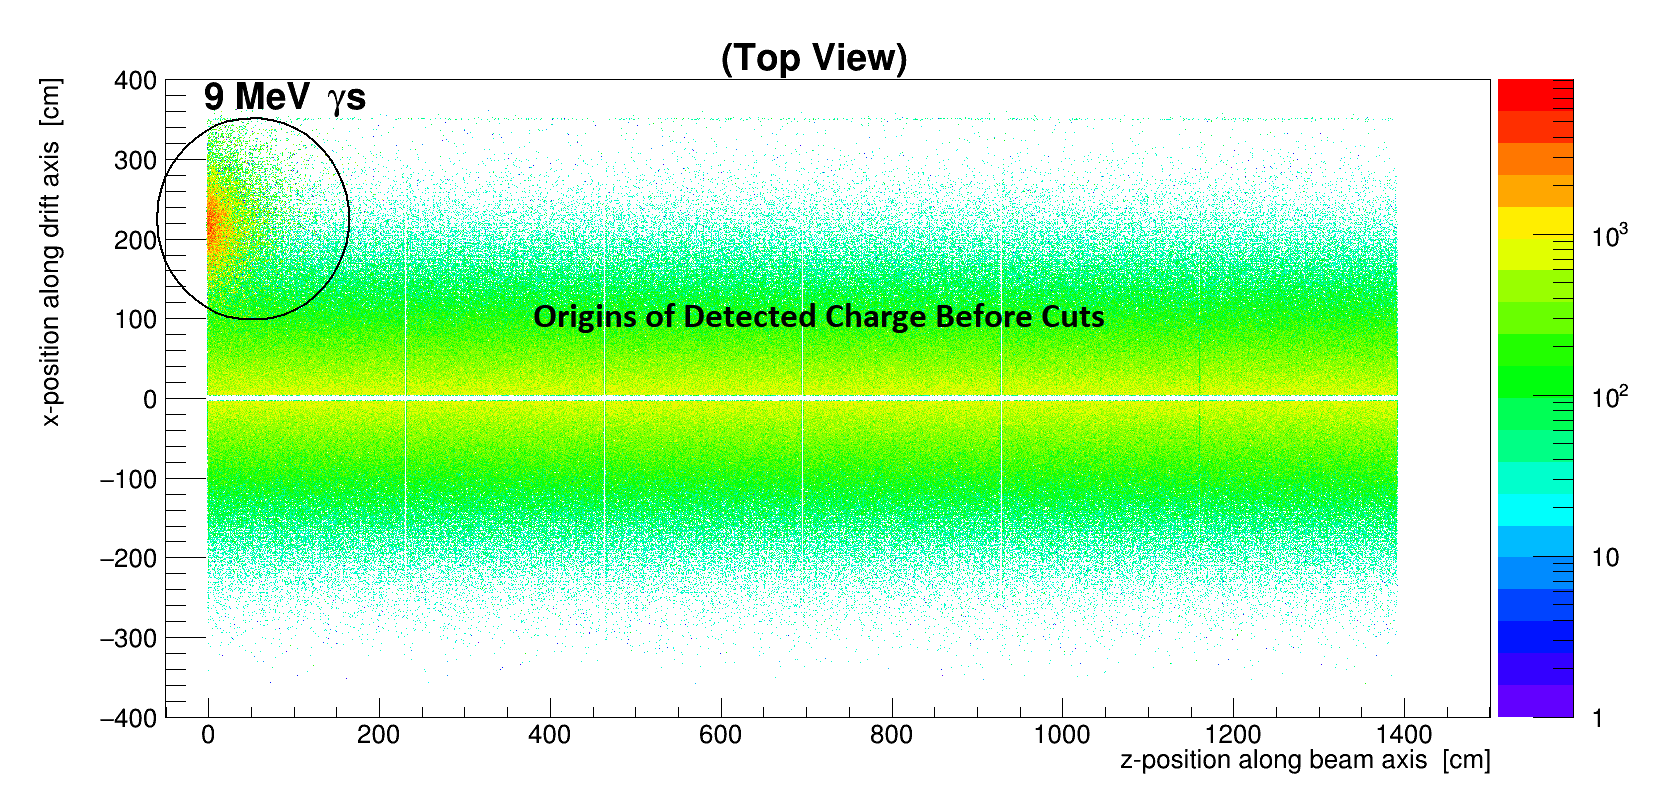
\includegraphics[width=1.0\linewidth]{9MeVgamma_withBG_LArSoft_v08_14_00_hiLY_originCHARGEcollected_TopView_TDR.png}
   (b)
   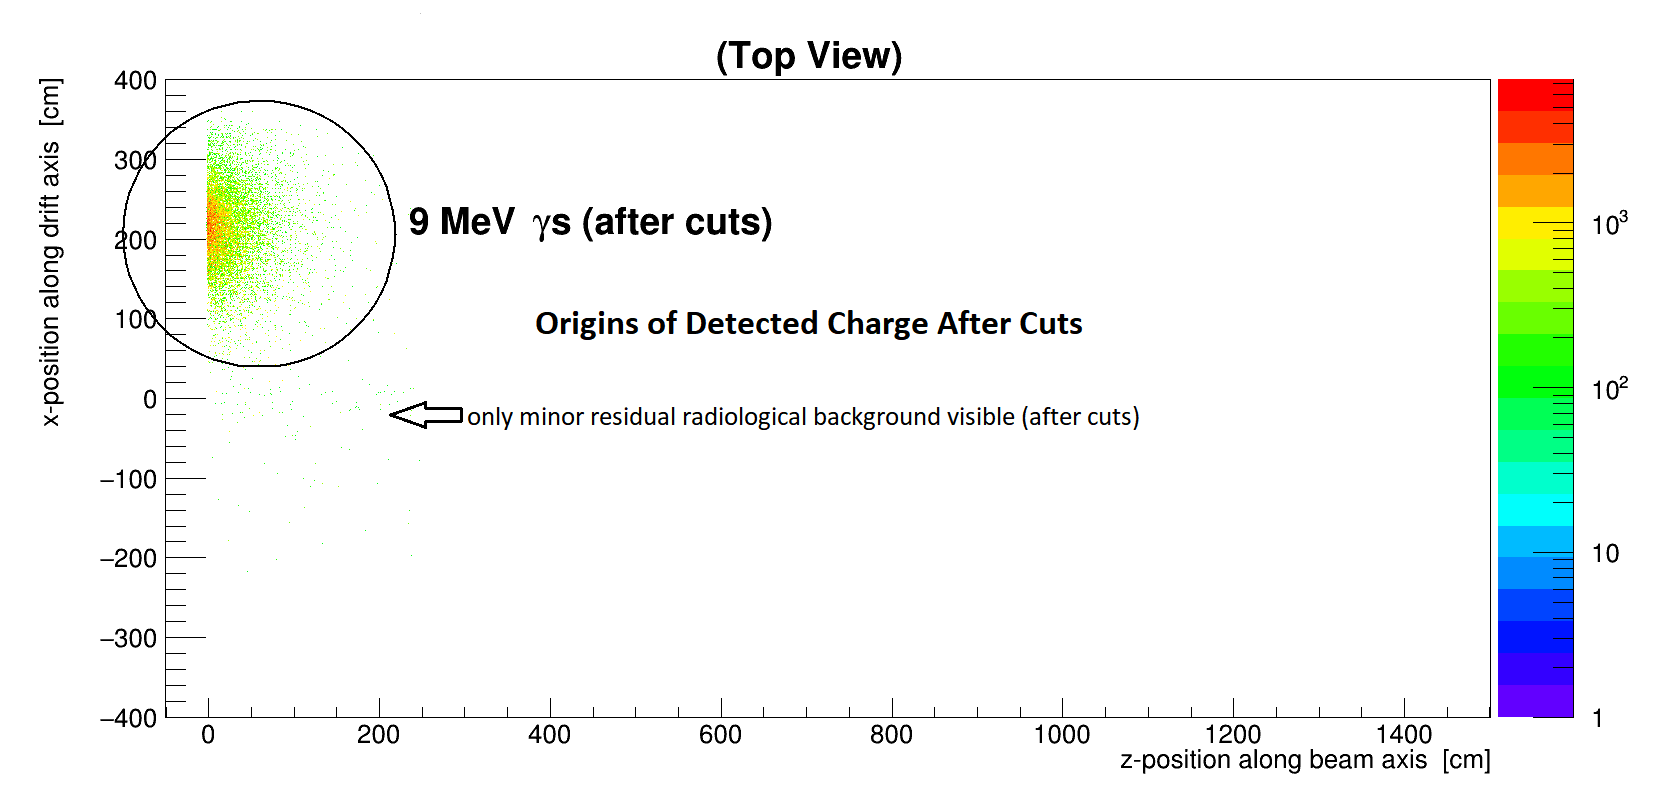
\includegraphics[width=1.0\linewidth]{9MeVgamma_withBG_LArSoft_v08_14_00_hiLY_originCHARGEcollected_TopView_cut_TDR.png}

%    \subfigure[a]{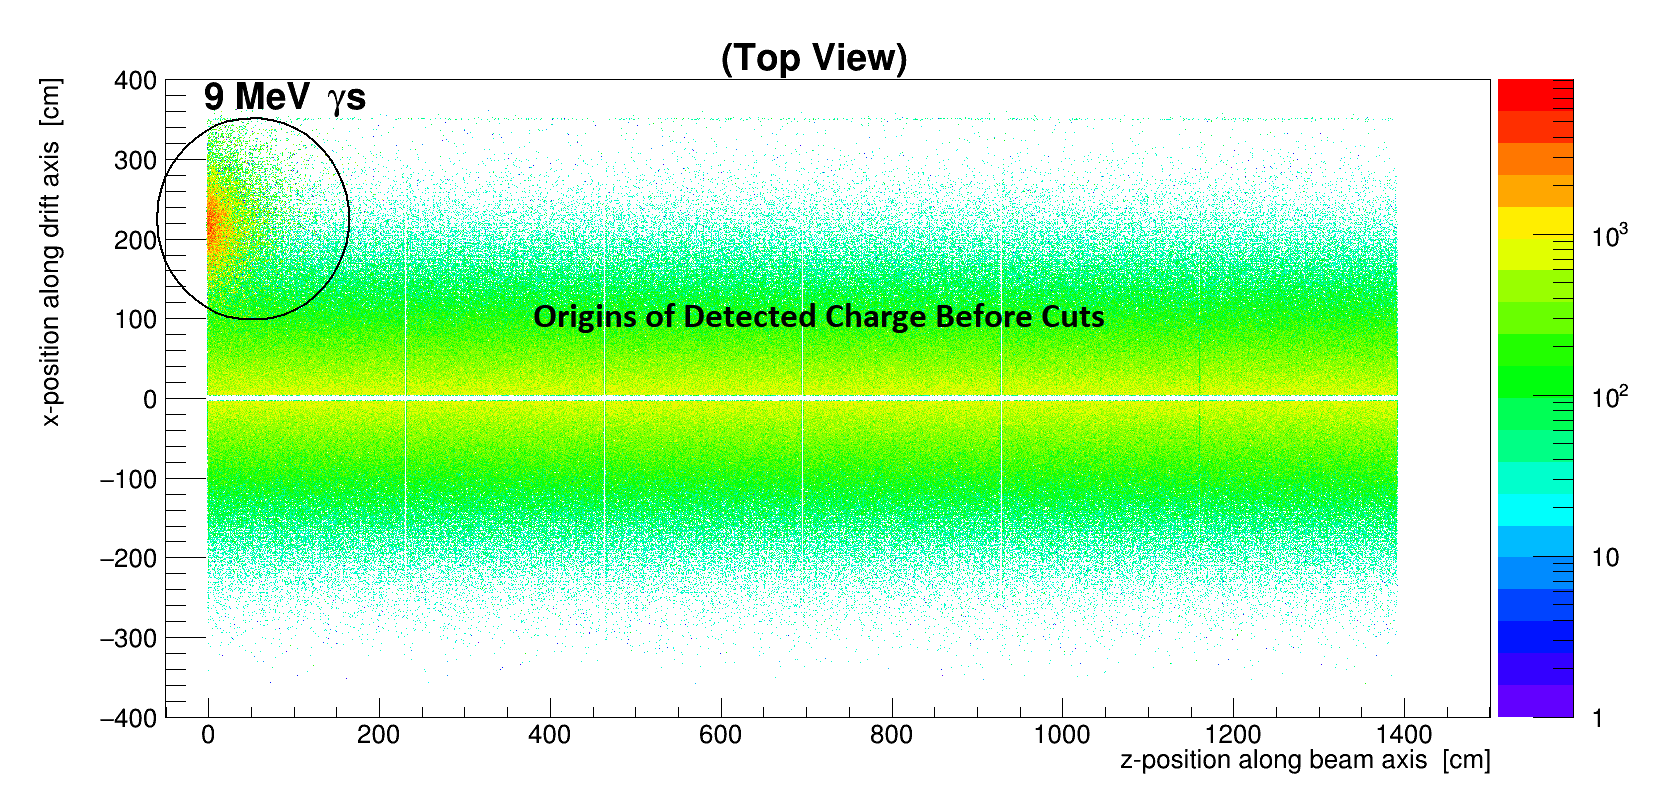
\includegraphics[width=1.0\linewidth]{9MeVgamma_withBG_LArSoft_v08_14_00_hiLY_originCHARGEcollected_TopView_TDR.png}}
%    \subfigure[b]{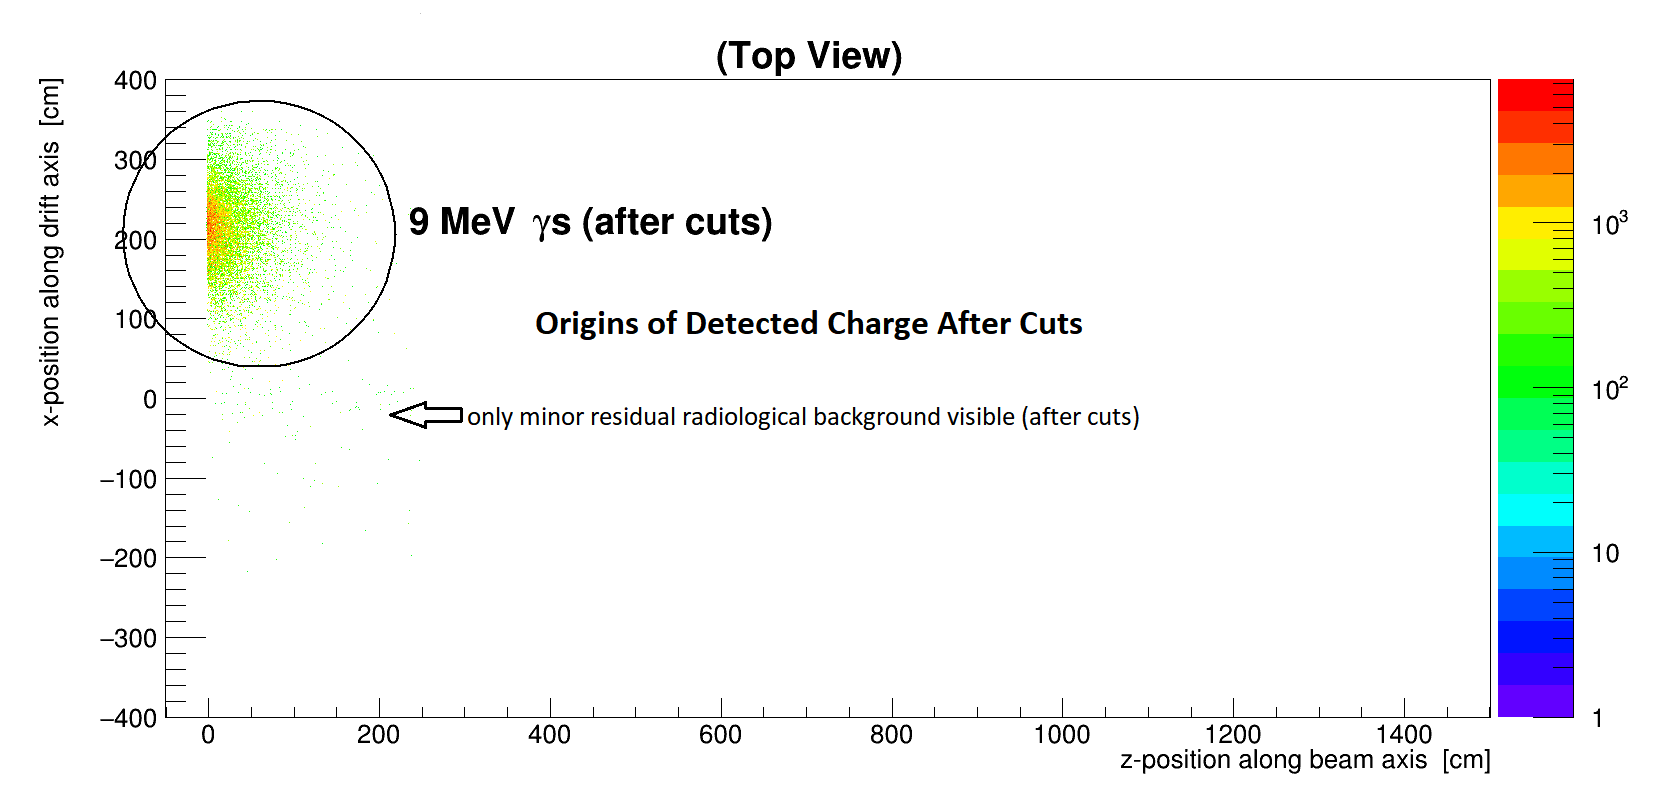
\includegraphics[width=1.0\linewidth]{9MeVgamma_withBG_LArSoft_v08_14_00_hiLY_originCHARGEcollected_TopView_cut_TDR.png}}
\end{dunefigure}

\begin{dunefigure}[Measured \efield and e$^-$ lifetime from \SI{9}{MeV} gamma; with radiological backgrounds]
{fig:rsds-fig2}
%{fig:9MeVgamma_withBG_LArSoft_v08_14_00_hiLY_DriftTimesEfield_ChargeSpectrumElectronLifetime_cut}
{Simulated measurements of (a) \efield strength from drift-time distribution, (b) electron lifetime from drift-time distribution, and (c) electron lifetime from charge distribution when electric field is unambiguously known from drift-time distribution. All spectra were created with applied selection cuts for a simulated 9~MeV $\gamma$-ray source with radiological backgrounds deployed at $z=$\SI{-40}{\cm} outside of the \dword{fc}, $x=$\SI{220}{\cm} away from the \dword{apa}, and $y=$\SI{300}{\cm} half-height of an upper endwall \dword{apa}. (Colors of histograms are matching colors of corresponding labels in each histogram.)}
\centering
    (a)
    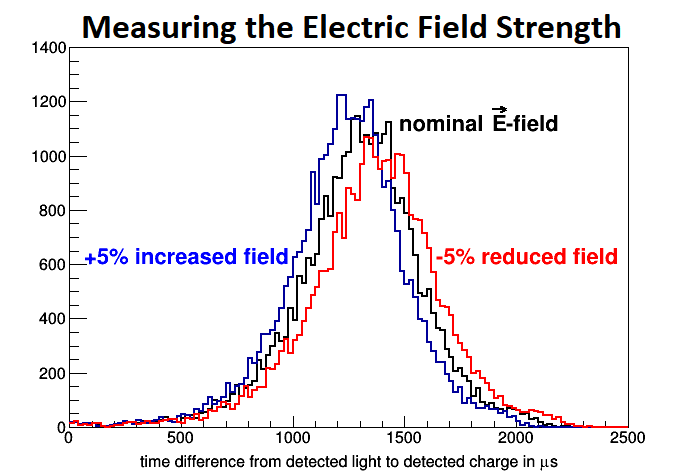
\includegraphics[width=0.45\linewidth]{9MeVgamma_withBG_LArSoft_v08_14_00_hiLY_EfieldDriftTimes_cut_TDR.png}
    (b)
    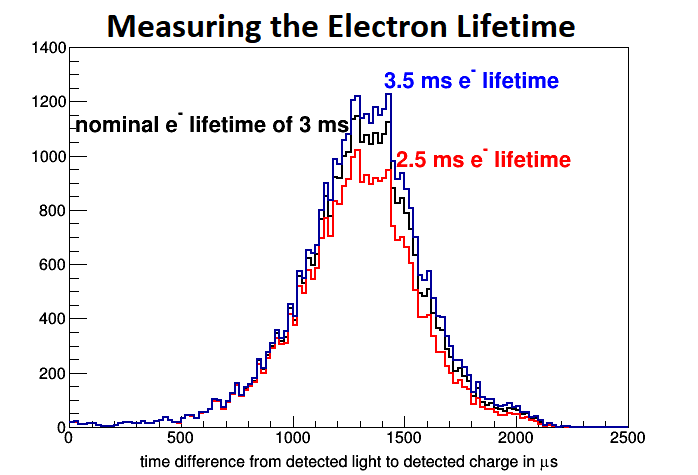
\includegraphics[width=0.45\linewidth]{9MeVgamma_withBG_LArSoft_v08_14_00_hiLY_eLifeTimeDriftTimes_cut_TDR.png}
    (c)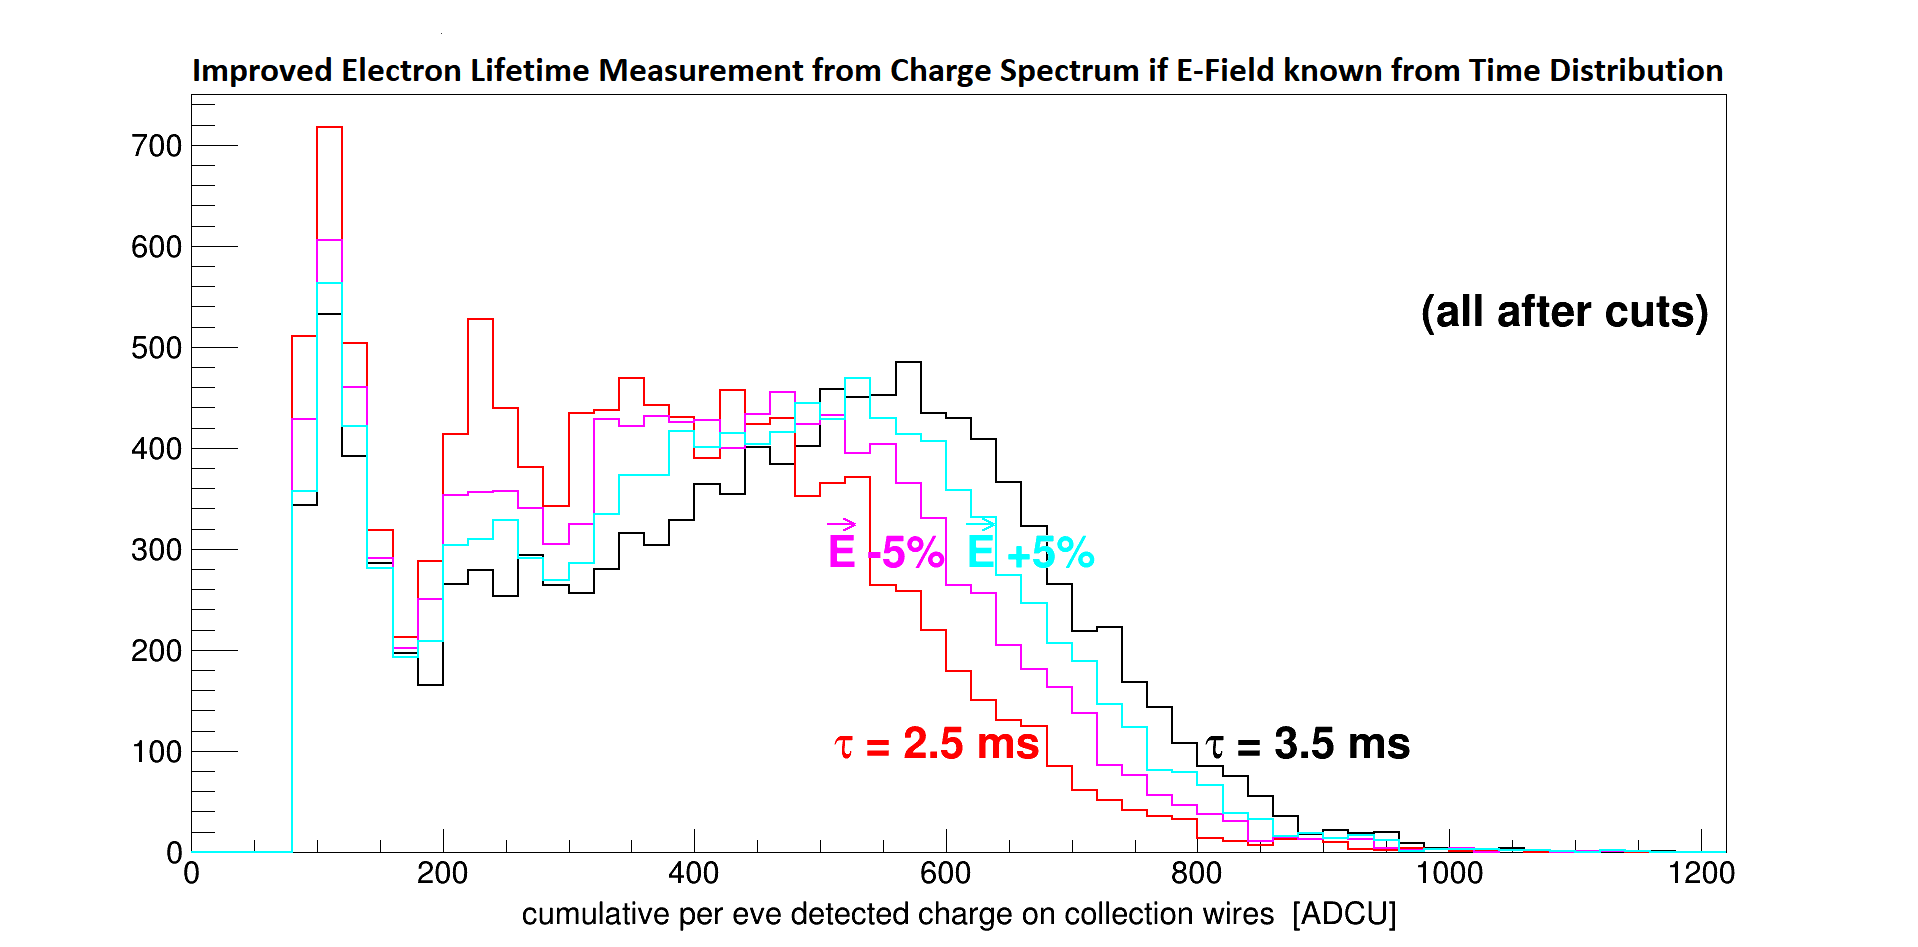
\includegraphics[width=1.0\linewidth]{9MeVgamma_withBG_LArSoft_v08_14_00_hiLY_chargeSpectrum_eLifeTimeEfield_cut_TDR.png}
    
%        \subfigure[a]{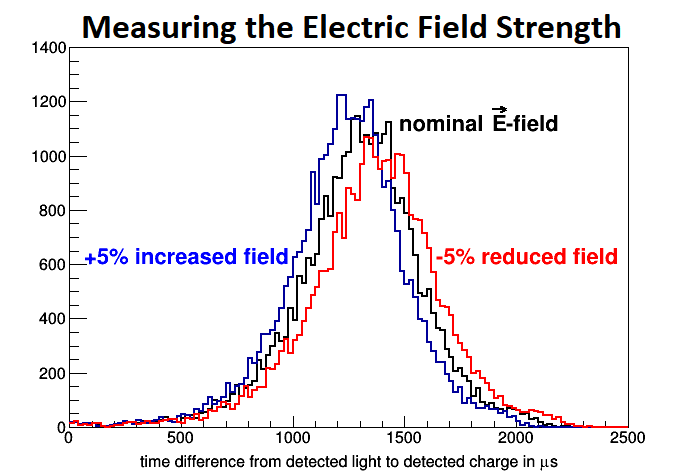
\includegraphics[width=0.45\linewidth]{9MeVgamma_withBG_LArSoft_v08_14_00_hiLY_EfieldDriftTimes_cut_TDR.png}}
%    \subfigure[b]{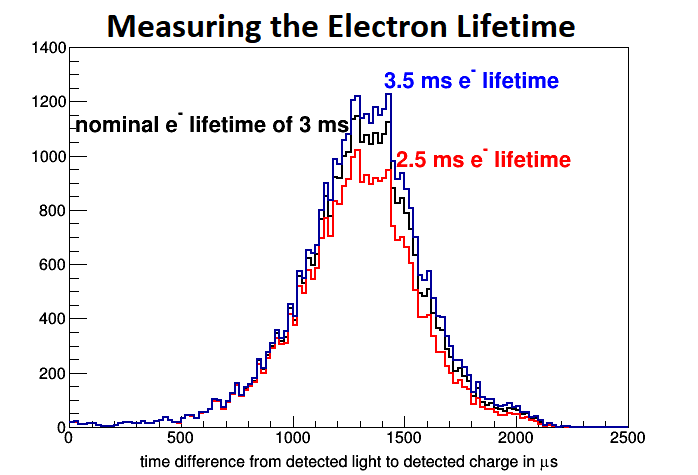
\includegraphics[width=0.45\linewidth]{9MeVgamma_withBG_LArSoft_v08_14_00_hiLY_eLifeTimeDriftTimes_cut_TDR.png}}
%    \subfigure[c]{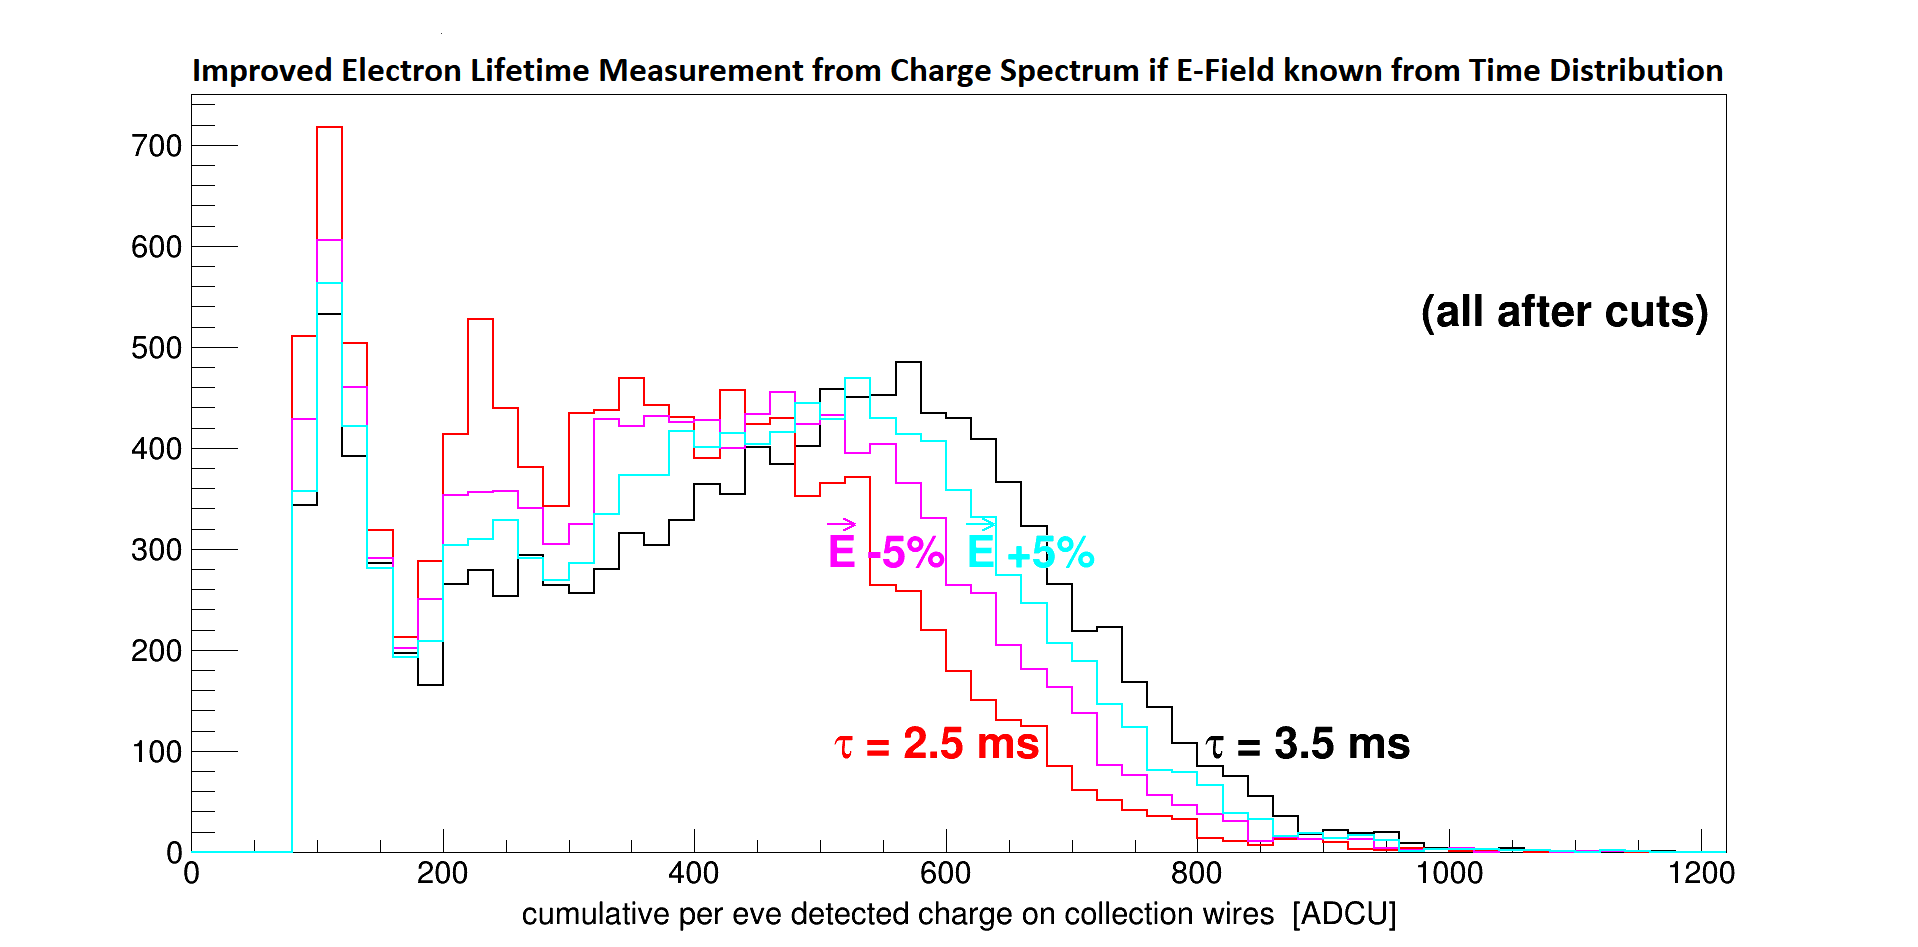
\includegraphics[width=1.0\linewidth]{9MeVgamma_withBG_LArSoft_v08_14_00_hiLY_chargeSpectrum_eLifeTimeEfield_cut_TDR.png}}
\end{dunefigure}

\begin{dunefigure}[Frequency of optical channel hits with gamma source;  with radiological backgrounds]
{fig:rsds-fig2plus}
%{fig:5MeValphaSource_zx_TDR_TopView}
{In LArSoft simulated change in frequency of optical channel hits with a simulated 9~MeV $\gamma$-ray source deployed at $z=$\SI{-40}{\cm} outside of the \dword{fc}, $x=$\SI{220}{\cm} away from the \dword{apa}, and $y=$\SI{300}{\cm} half-height of an upper endwall \dword{apa} with simulated expected radiological background.}
  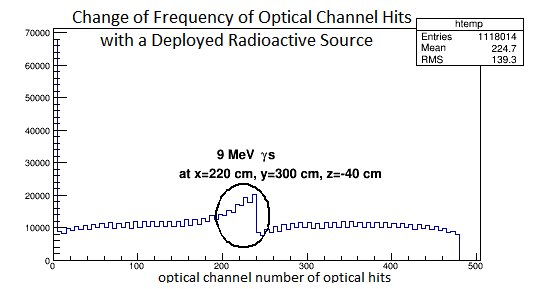
\includegraphics[width=0.6\linewidth]{ophit_opchannels_9MeVgammaSource_wBGs_LArSoft_v08_14_00_geo_v4_TDR.png}
\end{dunefigure}


\begin{dunefigure}[Detected light, charge from \SI{15}{MeV} gamma source; no radiological backgrounds]
{fig:rsds-fig3}
%{fig:5MeValphaSource_zx_TDR_TopView}
{In LArSoft backtracked origins of detected (a) photoelectrons and (b) charge for a simulated $^{40}$Ar($\alpha,\,\gamma$)$^{44}$Ca 15~MeV $\gamma$-ray source deployed at $z=$\SI{-40}{\cm} outside of the \dword{fc}, $x=$\SI{220}{\cm} away from the \dword{apa}, and $y=$\SI{300}{\cm} half-height of an upper endwall \dword{apa} without simulated expected radiological background.}
\centering
   (a)
   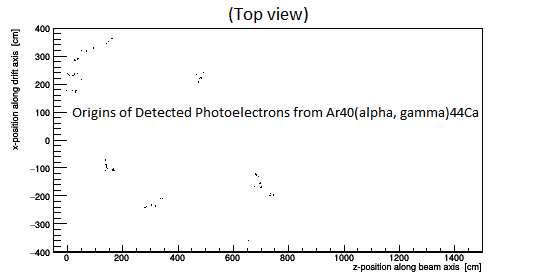
\includegraphics[width=0.455\linewidth]{5MeValphaSource_zx_pe_TDR.png}
   (b)
   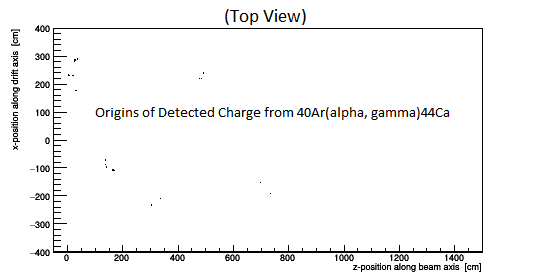
\includegraphics[width=0.455\linewidth]{5MeValphaSource_zx_adc_TDR.png}
\end{dunefigure}



\subsubsection{\dword{rsds} Design Validation}
\dword{protodune} forms the ultimate test to validate the design, operation and performance of the system. The cosmic induced background rate at \dword{protodune} is too high at the surface to detect responses to the \dword{dune} gamma source; a higher intensity source could be deployed to test the detector response and analysis method. However, tests of functionality,  reliability, and safety of the mechanical deployment system are needed to show the source can be deployed and retrieved with no issues.

\subsubsection{DAQ Requirements}
Section~\ref{sec:sp-calib-daqreq} provides an overall discussion of the Calibration and \dword{daq} interface. Here, the \dword{daq} requirements for the \dlong{rsds} are discussed. The radioactive source will not be triggerable by the \dword{mlt}.  Rather, it will deliver a tag to the \dword{mlt} and that tag will include a time stamp that can be used by the \dword{mlt} to issue a trigger command to the \dword{fe} readout.  The trigger command will have a standard readout window size of \SI{5.4}{\milli\s}, but to keep data rates manageable, the command will only be send to \dword{fe} readout buffers that are expected to be illuminated by the source. The localization of trigger commands thus reduces the data volume by \num{150}, if only one \dword{apa} is read out.

Nevertheless, if the rate of such a source is anywhere close to one per \SI{5.4}{\milli\s}, the detector would be running  continuously in the current scheme. Therefore we assume that the interaction rate in the detector is \SI{10}{\hertz} or less. The tag from the source will likely be much higher than this, because not all $\gamma$s interact in the active \dword{tpc} volume. Thus the radioactive source trigger will be a coincidence in the Module-Level Trigger between a low-energy trigger candidate from the illuminated \dword{apa}, and a source tag with a relevant time stamp.  With this rate, and with localization of events to one \dword{apa}, the total data volume would be

\begin{equation}
\num{8}~{\rm hours} \times \num{4}~{\rm FTs} \times \SI{10}{\hertz} \times \num{1.5}~{\rm Bytes}\times \SI{2}{\mega\hertz}\times \SI{5.4}{\milli\s}\times \num{2560}~{\rm channels} = \num{50}~{\rm TB/scan}.
\end{equation}

Running this calibration four times/year would yield \num{200}~TB of data in \SI{10}{\kt} per year.

\begin{dunetable}
[Calibration DAQ summary for RSDS]
{p{0.2\textwidth}p{0.15\textwidth}p{0.5\textwidth}}
{tab:calib-daq-rsds}
{Estimated \dword{daq} rate per year per \SI{10}{\kt} for the radioactive source system.}   
System & Data Volume (TB/year) & Assumptions  \\ \toprowrule
Proposed Radioactive Source System & \num{200} & Source rate < \SI{10}{\hertz}; single \dword{apa} readout,  lossless readout; \num{4} times/year   \\ 
\end{dunetable}           

\subsubsection{Risks}
The risks associated with the radioactive source system are described in Table~\ref{tab:risks:SP-FD-CAL-RSDS} along with appropriate mitigation strategies and the impact (low, medium or high risk levels) on probability, cost, and schedule post-mitigation.


% risk table values for subsystem SP-FD-CAL-RSDS
\begin{footnotesize}
%\begin{longtable}{p{0.18\textwidth}p{0.20\textwidth}p{0.32\textwidth}p{0.02\textwidth}p{0.02\textwidth}p{0.02\textwidth}}
\begin{longtable}{P{0.18\textwidth}P{0.20\textwidth}P{0.32\textwidth}P{0.02\textwidth}P{0.02\textwidth}P{0.02\textwidth}} 
\caption[Risks for SP-FD-CAL-RSDS]{Risks for SP-FD-CAL-RSDS (P=probability, C=cost, S=schedule) More information at \dshort{riskprob}. \fixmehl{ref \texttt{tab:risks:SP-FD-CAL-RSDS}}} \\
\rowcolor{dunesky}
ID & Risk & Mitigation & P & C & S  \\  \colhline
RT-SP-CAL-10 & Radioactive source swings into detector elements & Constrain the system with guide-wires & L & L & L \\  \colhline
RT-SP-CAL-11 & Radioactivity leak & Obtain rigorous source certification under high pressure and cryogenic temperatures & L & L & M \\  \colhline
RT-SP-CAL-12 & Source stuck or lost & Safe engineering margins, stronger fish-line and a torque limit in deployment system & L & M & L \\  \colhline
RT-SP-CAL-13 & Oxygen and nitrogen contamination & Leak checks before deployments & L & M & M \\  \colhline
RT-SP-CAL-14 & Light leak into the detector through purge-box & Light-tight purge box with an infrared camera for visual checks & L & L & L \\  \colhline
RT-SP-CAL-15 & Activation of the cryostat insulation & Activation studies and simulations & L & L & L \\  \colhline

\label{tab:risks:SP-FD-CAL-RSDS}
\end{longtable}
\end{footnotesize}


\begin{comment}
%SG: Old table of risks for RSDS.
\begin{dunetable}
[Calibration risks3]
{p{0.03\linewidth}p{0.4\linewidth}p{0.05\linewidth}p{0.4\linewidth}}
{tab:fdgen-calib-risks3}
{Possible risk scenarios for the radioactive source system along with mitigation strategies. The level of risk is indicated by letters ``H'', ``M'', and ``L'' corresponding to high, medium and low level risks.}   
No. & Risk  & Risk Level & Mitigation Strategy  \\ \toprowrule

10 & The deployed radioactive source can potentially swing into detector elements if not controlled or if large currents exist in the \dword{lar} & M & Guide-wires mitigate this risk.\\ \colhline

11 & Radioactivity could leak into the detector during a deployment. & L & Rigorous source certification under large pressure and cryogenic temperatures mitigates this risk.\\ \colhline

12 & The source could get stuck or lost in the detector. & L & Fish-line an order of magnitude stronger than needed to hold the weight, round edges of the moderator and a torque limit of the stepper motor will mitigate this risk.\\ \colhline

13 & Oxygen and nitrogen could get into the \dword{lar} in case the purge-box has a small leak. & M & Leak checks before deployments, purge-box in under-pressure inside w/r to the detector, will mitigate this risk.\\ \colhline

14 & Light could couple into the detector. & M &
Light-tight purge-box, internally equipped with an infra-red camera for visual checks will mitigate this risk.\\ \colhline

15 & The source activity can activate the cryostat insulation. & L & Detailed simulations/activation measurements can say what is a tolerable activity and the source activity can be chosen to be below that. \\ \colhline
\end{dunetable}
\end{comment}

\subsubsection{Installation, Integration, and Commissioning}
The first elements of the radioactive source guide system are installed before the \dword{tpc} elements on the end wall farthest from the \dword{tco} and as the last system, concurrent and coordinated with the alternative laser system (if any deployed), once the \dword{tpc} is installed before closing the \dword{tco}. The radioactive source deployment system is installed at the top of the cryostat and can be installed when \dword{dune} becomes operational.

The commissioning plan for the source deployment system will include a dummy source deployment (within 2 months of the commissioning) followed by first real source deployment (within 3 to 4 months of the commissioning) and a second real source deployment (within 6 months of the commissioning). Assuming stable detector conditions, the radioactive source will be deployed every half a year. Ideally, a deployment before and after a run period are desired so at least two data points are available for calibration. This also provides a check if the state of the system
has changed before and after the physics data run.
%If stability fluctuates for any reason (e.g., electronic response changes over time) at a particular location, one would want to deploy the source at that location once a month, or more often, depending on how bad the stability is.
It is estimated that it will take a few hours (e.g. 8 hours) to deploy the system at one feedthrough location and a full radioactive source calibration campaign might take %at least 
a week.

%\newpage
\subsubsection{Quality Control}
A mechanical test of the Double Chooz fish-line deployment system with an \dword{lar} mock-up column will be done in the high bay laboratory at South Dakota School of Mines and Technology. The ultimate test of the system will be done at \dword{protodune}. Safety checks will also be done for the source and for appropriate storage on the surface and underground. 

\subsubsection{Safety}
\label{sec:sp-calib-rsds-safety}
A composite source is used for the radioactive source system that consists  of \isotope{Cf}{252}, a strong neutron emitter, and \isotope{Ni}{58}, which, via the \isotope{Ni}{58}(n,$\gamma$)\isotope{Ni}{59} process, converts one of the \isotope{Cf}{252} fission neutrons, suitably moderated, to a monoenergetic \SI{9}{\MeV} gamma. This system also poses a radiation risk, which will be mitigated with a purge-box for handling, and a shielded storage box and an area with lockout-tagout procedures, also applied to the gate-valve on top of the cryostat. Material safety data sheets will be submitted to DUNE ES\&H and specific procedures will be developed for storage and handling of sources to meet FRCM requirements. These procedures will be reviewed and approved by SURF and Fermilab radiation safety officers. Sources that get deployed will be checked monthly to ensure they are not leaking. A designated shielded storage area will be assigned for sources and proper handling procedures will be reviewed periodically. A custodian will be assigned to each shielded source.
 

%%%%%%%%%%%%%%%%%%%%%%%%%%%%%%%%%%%%%%%%%%%%%%%%%%%%%%%
%\section{Additional Systems Considered: External Muon Tracker}
%\label{sec:sp-calib-addl}
 
%%%%%%%%%%%%%%%%%%%%%%%%%%%%
%\subsection{External Muon Tagger}
%\fixme{you can't have just one subsection; if it's only the muon tagger, then let's put this in the section heading}
%\input{vol-sp/ch-sp-emt}

%%%%%%%%%%%%%%%%%%%%%%%%%%%%%%%%%%%%%%%%%%%%%%%%%%%%%%%
%\section{Cryostat Configuration for Calibration}
%\label{sec:sp-calib-cryocfg}


%%%%%%%%%%%%%%%%%%%%%%%%%%%%%%%%%%%%%%%%%%%%%%%%%%%%%%%  Anne changed from subsection to section
\section{DAQ Requirements}
\label{sec:sp-calib-daqreq}
%\fixme{SG: Done. JM: Done. (changed "DC" to continuously).\\
%KM/JM: Plesae check. Waiting on two things from Josh (What is "DC" used in RAS section; and which section he is referring to in the first two paragraphs?\\
%JM: Probably the DAQ Chapter of the TDR. Need to check w/ Tim/Sam if this is the right reference.}
 
%\section{DAQ Requirements}
%\label{sec:sp-calib-daqreq}

The calibration systems must interface with the DUNE data acquisition system, discussed in detail in Section~\ref{sec:daq}.
The primary interface with calibrations will be through the DUNE timing system, which is responsible for providing synchronization across all subsystems and absolute time stamps, as well as for distributing triggers. Whenever possible, it is preferred that subsystems like calibrations are triggered {\it by} the DAQ rather than providing a trigger {\it to} the DAQ. Therefore the calibration systems must be designed to accept such triggers (which will have the form of a time stamp for when a trigger should occur) and it must have a way of accepting general timing information so that it is synchronized to the rest of DUNE.

Each calibration system will nevertheless be handled slightly differently, and each will have a different way for the DAQ to handle its data.  The calibration systems could easily dominate the entire data volume for DUNE, and thus exceptions to the standard triggering and readout discussed in Section~\ref{sec:daq} are needed. We discuss below these details and the associated differences.
           
\begin{dunetable}
[Calibration DAQ summary]
{p{0.2\textwidth}p{0.15\textwidth}p{0.5\textwidth}}
{tab:calib-daq}
{Estimated DAQ rates per year per 10~kton for various calibration systems.}   
System & Data Volume (TB/year) & Assumptions  \\ \toprowrule
Ionization Laser System & 185 & 800k laser pulses, 10x10x10 cm voxel sizes, a 100~$\mu$s zero suppression window (lossy readout), and 2 times/year  \\ \colhline
Neutron Source System & 84 & 10$^{6}$~neutrons/pulse, 1000 neutron captures/m$^{3}$, 1300 observed neutron captures per pulse, 6~times/year  \\ \colhline
Proposed Radioactive Source System & 200 & Source rate < 10~Hz; single fragment readout,  lossless readout; 4 times/year   \\ \colhline

\end{dunetable}           
           
\subsubsection{Laser System}

%The proposed laser source is the only practical way to unambiguously measure the electric field vectors within the detector. 
The \efield vector from ionization laser calibration is determined by looking at the deflection of crossing laser tracks within detector voxels. The voxels are currently estimated at the size of $10\times10\times10~{\rm cm}^3$. Because any given laser track
illuminates many such voxels, one laser pulse can be used for multiple
measurements---essentially the number that matters is the area of each voxel.
The number of total laser ``events'' are estimated to be 800,000---about half the rate of cosmic rays, and thus nominally a substantial total data volume.

Fortunately, unlike every other event type in the detector, the laser track has both a reasonably well known position and time; thus tight zero-suppression can be applied for both collection and induction plane wires. %Brett Viren suggests that 
A 100~$\mu$s zero suppression window is estimated to be wide enough to
avoid windowing problems in the induction plane wire deconvolution process, and we
therefore assume such a window for the laser pulses. Note that the zero
suppression happens {\it after} the trigger, not at the front-end or in the DAQ
readout; thus the rate that the laser can be run will have to take into account
the bandwidth through the Event Builder (where the zero-suppression would
occur). From the standpoint of data volume, however, the total assuming the
100~$\mu$s zero-suppression window is:
\begin{equation}
800,000/{\rm scan/10~kton} \times 100\mu{\rm s} \times 1.5{\rm Bytes/sample}\times 2~{\rm MHz}\times 384000~{\rm channels}   = 92~{\rm TB/scan/10~kton}   
\end{equation}

If such a calibration scan were done twice/year, then the total annual data volume for the laser is 184~TB/year/10~kton.

\subsubsection{Pulsed Neutron Source}
%\todo{SG: JW to update this text and the number in the DAQ table 1.3.}
%There are two radioactive sources suggested to provide low-energy calibration data for DUNE: a neutron generator source, and a $\gamma$ source. 

The pulsed neutron source system creates a burst of neutrons which
%, because of the interesting neutron cross section of argon, 
get captured throughout a large fraction of the total cryostat volume. From a triggering and data volume
standpoint, this is very convenient: the existing scheme of taking 5.4~ms of data for each trigger means all of these neutrons will be collected in a single DUNE event. Thus the data volume is simply 6.22~GB times the total number of such pulses, but these are likely to be few: a single burst can produce thousands of neutrons whose $t_0$ is known up to the neutron capture time of 200~$\mu$s or so.


Typically, a commercial $DD$ neutron generator produces 10$^{5}$ - 10$^{8}$ neutrons/pulse, depending on the adjustable pulse width. The current assumption for neutron yield from the $DD$ generator is 10$^{6}$ neutrons per pulse\footnote{Ideal assumption based on $DD$ generators that produce highest neutron yield with a pulse width less than 100~$\mu$s. Such type of $DD$ generators are being developed in labs; commercial devices may require further development to reach this level of performance.}. With the current deployment designs in figure~\ref{fig:PNS_source_design}, about 1300 neutron captures per $DD$ generator pulse are expected to be observed inside a 10~kt module. As the suggested number for localized energy calibration is 1000 neutron captures per m$^{3}$, a total number of 4600 pulses would be needed for the calibration of a 10~kt module. Assuming there will be two identical Pulsed Neutron Sources operating in synchronization mode, 2300 pulses are needed for each calibration run. Therefore, the total data volume per run would be
\begin{equation}
2300~Pulses \times 1.5~{\rm Bytes}\times
2~{\rm MHz}\times 5.4~{\rm ms}\times384000~{\rm channels} = 14~{\rm TB/run}.
\end{equation}
Running the Pulsed Neutron Source calibration system every two months would result in a total data volume of 84~TB per 10~kton per year and running 12 times/year would result in 168~TB/year per 10~kton. 

\subsubsection{Proposed Radioactive Source System}

The proposed $\gamma$ source is somewhat more complicated to handle in the DAQ, depending on its rate. An initial proposal suggests 8 hour runs at four feedthroughs, and because only a single APA is being illuminated typically, the Module Level trigger could reduce the total data rate by issuing trigger
commands only to the readout of the currently active APA. Nevertheless, if the rate of such a source is anywhere close to one per 5.4~ms, the detector would be running 
continuously 
%in ``DC'' 
in the current scheme. Therefore we assume that the
interaction rate in the detector is 10~Hz or less.  With this rate, and with localization of events to one APA, the total data volume would be
\begin{equation}
8~{\rm hours} \times 4~{\rm FTs} \times 10~Hz \times 1.5~{\rm Bytes}\times
2~{\rm MHz}\times 5.4~{\rm ms}\times2560~{\rm channels} = 50~{\rm TB/scan}.
\end{equation}
Running this calibration 4 times/year would yield 200~TB of data in 10~kton per year.





\begin{comment}
%SG: This is not under the scope of this chapter. Needs to be moved to physics. 
\subsubsection{Intrinsic Radioactivity}

        Mike Mooney has suggested using the intrinsic $^{39}$Ar as a
calibration source. This has many advantages over either of the radioactive
source calibrations, in particular the known level of $^{39}$Ar, its uniform
distribution in the detector, and the fact that it is always there and
therefore integrates correctly over the detector livetime. The difficulty is
that because any individual $^{39}$Ar event's $x$ position is not known
(because there is no $t_0$, the distribution of these events must be used to
make measurements, thus requiring fairly high statistics.

        Mooney's proposal is that roughly 250,000 $^{39}$Ar can provide a 1\%
measurement of electron lifetime. (Note that 1\% is a reaonable goal;
if the lifetime and maximum drift time are the same, this results
in a 2\% uncertainty on energy scale which would begin to compromise DUNE's
physics program). This number of events is easily obtained with the existing
random triggers as well as every other trigger source excluding laser pulses
and front-end calibrations.

        Like all other parameters that must be calibrated, however, what is not
clear is what the spatial and temporal variations will be in the detector.
Other LAr TPCs have performed lifetime calibrations daily (using cosmic rays
primarily), and a pixelization of 1~m$^2$ is not unreasonable, leading to a
need for 250,000 events for every m$^2$ in the detector each day, or about a
1~Hz trigger rate.

        In the existing scheme, this would be overwhelmingly the dominant
source of data. Thus either the pixelization would need to be reduced (say, to
each of the TPC volumes) or a zero-suppression scheme would have to be used.
Such a zero-suppression scheme would happen post-trigger---for example, running
random triggers at 1~Hz and based upon that trigger type, zero suppressing
signals. In the current scheme, this would happen in the Event Builder but at
1~Hz the data rate would be too high. To do zero suppression upstream---say in
the APA-level readout---based on the trigger type will likely require more
hardware resources.
\end{comment}

%\subsection{External Muon Tracker}

%        An External Muon Tracker (EMT) has also been proposed, likely as a scintillator-bar telescope at the front face of the detector. The EMT would be intended to trigger on rock muons and provide a known entry position and direction for these. It is thus the only way to test reconstruction in the DUNE FD for a sample of events in the same energy regime as the beam events.

%        Because the EMT is measuring events that will already be triggered by the TPC, the additional data volume comes only from the scintillator counters themselves. Because the only information needed for these events is the time of a hit in each counter, and because only four counters are likely to be hit by each muon (two planes of $x$ and $y$), the additional data rate from the EMT is very small.  If we limit ourselves to just the rock muons and assume that four counters are hit resulting in 4 12-bit words/counter (one charge and one time each, plus the counter ID and a local timestamp, then we get a yearly total data volume of
%\begin{equation}
%735{\rm year/10 ktonne} \times 24~{\rm B/event} = 17.6~{\rm kB/year}   
%\end{equation}

%%%%%%%%%%%%%%%%%%%%%%%%%%%%%%%%%%%%%%%%%%%%%%%%%%%%%%% Anne changed from subsection to section
\section{Validation of Calibration Hardware Systems}
\label{sec:sp-calib-val}

%%%%%%%%%%%%%%%%%%%%%%%%%%%%
%\subsection{Validation of Calibration Hardware Systems}

All calibration designs presented in the previous section require full system validation before being deployed in the \dword{dune} \dword{fd}. Here, we describe the validation of a complete baseline design and some of the alternative designs described in the Appendix.

Although laser calibration systems are being operated in other \dword{lartpc} experiments (e.g., \dword{microboone}, future \dword{sbnd} runs), they have stringent requirements in terms of mechanical and optical precision , long-term reliability, laser track length, performance of the \dword{lbls}, \dword{daq} interface, and effect on \efield, especially due to the \dword{fc} penetration. 
%with alternative design options
All of these lead to corresponding goals for a test installation and operation in \dword{pdsp} that could be done in the post-LS2 run. As Figure~\ref{fig:protoDUNESP_topView_marked} shows, \dword{pdsp} has ports of the same size as the \dword{dune} \dword{fd} that could be used for these tests. If a pair of ports can be used, then one could even have crossing tracks within a single drift volume. If one of the ports external to the \dword{tpc} can be used, then we would test the double-rotary alternative system described in Section~\ref{sec:sp-calib-laser-alter} and aimed at improving the coverage from the end-wall locations.

\begin{dunefigure}[Top view of the \dshort{pdsp} cryostat showing various penetrations]{fig:protoDUNESP_topView_marked}
{Top view of the \dword{pdsp} cryostat showing various penetrations. Ports marked in red are free and could be used to test the calibration systems. The four largest ports have the same diameter (\SI{250}{\milli\m}) as the calibration ports of DUNE \dword{fd}, and are located over the \dword{tpc}. The largest ports at the right side corners of the cryostat are the human access ports.}
\includegraphics[height=4.0in]{protoDUNESP_topView_marked.png}
\end{dunefigure}

The goal for validation would be to test all aspects of the system design, installation, alignment, operation, interfaces with \dword{daq}, and analysis, among others. \dword{pdsp}, because it is located at the surface, could measure the \efield map with cosmic rays to compare with the one from the laser system to improve the analysis methods or identify weak aspects in the design. An important design parameter is the length of a laser track. Our design assumes that \SI{20}{\m} is possible. \dword{microboone} has demonstrated only up to \SI{10}{\m}, but the track could be longer, depending on laser intensity. Measurements are limited by the size of the detector, but one way to gain information on longer tracks is to make a scan with low laser intensities, so that the end of the track is  visible, and register how the maximum obtained track length scales with intensity. An extrapolation to the \dword{dune} \dword{fd} laser intensity would tell us the maximum length possible. Such a measurement could also be done at \dword{microboone} or \dword{sbnd}.

An important aspect of the development plan, to be carried out at \dword{pdsp2}, is the characterization of the charge created by the laser beam ionization as a function of distance travelled in the \dword{lar} and the laser beam intensity. This dependence is thought to be affected by self-focusing effects due to the high light intensity, but it can be studied by measuring the collected charge distribution from a series of tracks close, and parallel, to the \dword{apa}s in order to break any correlations with the electron lifetime. This measured charge function could then be used with tracks in different directions to obtain a measurement of electron lifetime, which would significantly increase the capabilities of the laser system. 

The pulsed neutron source is a new idea never used in other experiments, so a \dword{pdsp2} test is essential. The corner human access ports similar to the ones in the \dword{dune} \dword{fd} could be used for this test.


In addition to dedicated hardware validation runs at \dword{pdsp2}, other \dword{lar} experiments provide ample opportunities to develop and validate calibration tools and techniques, especially those relevant to the hardware being deployed. For example, the \dword{microboone} experiment is currently leading the development of analysis methods using laser data to extract an \efield map. Energy calibration techniques and related software tools are also being developed at various experiments (\dword{microboone}, ICARUS, \dword{lariat}, \dword{protodune}) that involve estimating and propagating uncertainties like \efield distortions, recombination, and other effects into physics signals. Other calibration related developments include \dword{daq} and calibration database design, all of which are being improved at \dword{sbn} and \dword{protodune}.
 


%%%%%%%%%%%%%%%%%%%%%%%%%%%%%%%%%%%%%%%%%%%%%%%%%%%%%%%
\section{Organization and Management}
\label{sec:sp-calib-org}


The calibration consortium was formed in November 2018 as a joint single and dual phase consortium, with a consortium leader and a technical leader. Figure~\ref{fig:orgchart} shows he organization of the consortium. The calibration consortium board currently comprises institutional representatives from 11 institutions as shown in Table~\ref{tab:gen-calib-org}. The consortium leader is the spokesperson for the consortium and responsible for the overall scientific program and management of the group. The technical leader of the consortium is responsible for managing the project for the group. 

The consortium's initial mandate is the design and prototyping of a laser calibration system, a neutron generator, and possibly a radioactive source system, so the consortium is organized into three working groups, each dedicated to one system. Each group has a designated working group leader.
The \dword{tdr} editors are responsible for the overall editing and delivery of the \dword{tdr} document.


\begin{dunefigure}[Organizational chart for the calibration consortium]{fig:orgchart}
{Organizational chart for the calibration consortium.}
\includegraphics[height=3.0in]{orgchart.png}
\end{dunefigure}


\begin{dunetable}
[Calibration Consortium Institutions]
{lc}
{tab:gen-calib-org}
{Current Calibration Consortium Board Institutional Members and Countries.}
Member Institute     &  Country       \\
LIP & Portugal \\ \colhline
University of Bern (Bern) & Switzerland \\ \colhline
University of Tennessee, Knoxville (UTK) & USA \\ \colhline
Michigan State University (MSU) & USA \\ \colhline
Colorado State University (CSU) & USA \\ \colhline
University of Iowa & USA \\ \colhline
University of Hawaii (Hawaii) & USA \\ \colhline
University of Pittsburgh (Pitt) & USA \\ \colhline
Boston University (BU) & USA \\ \colhline
University of California, Davis (UC Davis)& USA \\ \colhline
South Dakota School of Mines and Technology (SDSMT) & USA \\ 
\end{dunetable}

In addition, Figure~\ref{fig:orgchart} shows several liaison roles currently being established 
%\todo{These are being established after we have had initial interfaces and critical issues clarified} 
to facilitate connections with other groups and activities:
\begin{itemize}
    \item Detector integration and installation,
    \item Electrical and safety issues,
    \item \dword{daq},
    \item Computing,
    \item Cryogenic instrumentation and slow controls (CISC),
    \item Cold electronics,
    \item High voltage,
    \item Photon Detection System.
\end{itemize}

%\fixme{KM adjusted above from "planned" to state will exist by Summer 2019}

Currently, new institutions are added to the consortium  following an expression of interest from the interested institute and upon obtaining consensus from the current consortium board members.

%if the consortium board members agree, new members are added from other institutions if the new institutions express an interest through a petition to the board.

%There are 11 institutes in the Consortium and, as the activities progress from design to prototyping, formalization of a Consortium Board is also planned.

%%%%%%%%%%%%%%%%%%%%%%%%%%%%%%%%%%%%%%%%%%%%%%%%%%%%%%%

\section{Interfaces}
\label{sec:sp-calib-intfc}


Interfaces between calibration and other consortia have been identified and appropriate documents have been developed. %We plan to have first full drafts of the interface documents by June 2019. 
The documents are currently maintained in the \dword{cern} Engineering and Equipment Data Management Service (EDMS) database, with a \dword{tdr} snapshot kept in the \dword{dune} document database (DocDB).
%The documents are currently maintained in the the \dword{cern} EDMS database
\dword{dune} document database (DocDB). %\fixme{This has not been defined in either the common glossary or in the glossary for this document.}
%\todo{documents being prepared now}
A brief summary is provided in this section. Table~\ref{tab:fdgen-calib-interfaces} lists the interfaces and corresponding DocDB document numbers. 
The main systems calibration has interfaces with are \dword{hv}, \dword{pds}, and \dword{daq}, and the important issues that must be considered are listed below.

\begin{description}
    \item[HV] Evaluate the effect of the calibration hardware on the \efield due to laser system periscopes and \dword{fc} penetration. %This needs to be done for the alternative design described in the appendix, in which the \dword{fc} is penetrated, but should also be done in the baseline design, for which there is no penetration of the \dword{fc}. 
    %\fixme{This is not clear. FC penetrations for laser? is that a second evaluation that must be made with the effect of the incident laser beam being a third evaluation? Basically, the previous phrase must be a complete sentence with full content.} 
    Evaluate the effect of the incident laser beam on the \dword{cpa} material (Kapton); Integrate the hardware of the %alternative 
    photoelectron laser system (targets) and the \dword{lbls} (diodes) within the \dword{hv} system components. Ensure that the radioactive source deployment is in a safe field region and cannot do mechanical harm to the \dword{fc}.
    \item[PDS] Evaluate long term effects of laser light, even if just diffuse or reflected, on the scintillating components (\dword{tpb} plates) of the \dword{pds}; establish a laser run plan to avoid direct hits; evaluate the effect of laser light on alternative \dword{pds} ideas, such as having reflectors on the \dwords{cpa}; validate light response model and triggering for low energy signals. 
    %\fixme{Note how PDS is phrased. The other two items should be phrased similarly. Begin with a verb (evaluate, establish, evaluate, validate). Then follow each item in the list with a semicolon as in this section.}
    \item[DAQ] Evaluate \dword{daq} constraints on the total volume of calibration data that can be acquired; develop strategies to maximize the efficiency of data taking with data reduction methods; study how to implement a way for the calibration systems to receive trigger signals from \dword{daq} to maximize supernova live time. More details on this are presented in Section~\ref{sec:sp-calib-daqreq}.
    %\item[Computing] Evaluate any additional semi-offline processing needs. Coordinate needs for calibration databases. 
\end{description}

Integrating and installing calibration devices will interfere with other devices, requiring coordination with the appropriate consortia as needed. Similarly, calibration will have significant interfaces at several levels with cryostat and facilities in coordinating resources for assembly, integration, installation, and commissioning (e.g., networking, cabling, safety). Rack space distribution and interaction between calibration and systems from other consortia will be managed by \dword{tc} in consultation with those consortia.

\begin{dunetable}
[Calibration system interfaces]
{p{0.14\textwidth}p{0.40\textwidth}p{0.14\textwidth}}
{tab:fdgen-calib-interfaces}
{Calibration Consortium Interface Links.}   
\small
Interfacing System & Description & Reference \\ \toprowrule
\dshort{hv}	&
effect of calibration hardware (laser and radioactive source) on \efield and field cage; laser light effect on \dshort{cpa} materials, field cage penetrations; attachment of positioning targets to HV supports 
& \citedocdb{7066} 
\\ \colhline
\dword{pds}	& 
effect of laser light on \dshort{pds}, reflectors on the \dshort{cpa}s (if any); validation of light response and triggering for low energy signals 
& \citedocdb{7051}
\\ \colhline
\dshort{daq}	& 
DAQ constraint on total volume of the calibration data; receiving triggers from DAQ
& \citedocdb{7069}  
\\ \colhline
\dshort{cisc} &
multi-functional \dshort{cisc}/calibration ports; space sharing around ports; fluid flow validation; slow controls and monitoring for calibration quantities 
& \citedocdb{7072} 
\\ \colhline
TPC Electronics	         &  
Noise, electronics calibration
& \citedocdb{7054}  
\\ \colhline
\dshort{apa}	&
\dshort{apa} alignment studies using laser and impact on calibrations
& \citedocdb{7048} 
\\ \colhline
Physics	&
tools to study impact of calibrations on physics
& \citedocdb{6865}  
\\ \colhline
Software and Computing	  &
Calibration database design and maintenance
& \citedocdb{6868} 
\\ \colhline
TC Facility              &   
Significant interfaces at multiple levels   
& \citedocdb{6829}   \\ \colhline
TC Installation     	  &     
Significant interfaces at multiple levels
& \citedocdb{6847}    \\ 

\end{dunetable}



%%%%%%%%%%%%%%%%%%%%%%%%%%%%%%%%%%%%%%%%%%%%%%%%%%%%%%%
\section{Cost and Labor}
\label{sec:sp-calib-cost}


%\fixme{KM/JM: Done; SG check?}
%KM: I am OK with this, let's see what the editors hate. \fixme{SG: done checking; 1. photoelectron laser missing from the table. Added it. 2. Updated the text to clearly state what the cost estimates include; 3. added some description for labor and a table with placeholders for actual labor hours. 4. The way it is currently split in the cost table, using the same rows will be tricky for labor hours. E.g. for the laser itself, no significant labor is associated. So, for the labor table, although it inconsistent with the cost table, I listed each of our devices as one entity. check if you are okay with this. Alternatively, we can lump everything into one system for the cost table as well so both tables are consistent which is what is expected from main editors. 5. I added a new category for labor, "physics & simulation" as those hours will also need to accounted for. }

\begin{dunetable}
[Calibration System Cost Summary]
{p{0.15\textwidth}p{0.1\textwidth}p{0.15\textwidth}p{0.4\textwidth}}
{tab:calib-cost}
{Cost estimates for different calibration subsystems.  All cost estimates include packing and shipping costs.}   
System & Quantity & Cost (under development) (k\$ US) & Description \\ \toprowrule
laser & 17 & - & high intensity laser source for laser system  \\ \colhline
laser optics module & 20 & -&  insulator ingress into detector and flange interface, mirrors, power, cables for laser system, and positioning system \\ \colhline
Photoelectron system & 4000 & - & includes targets to be mounted, both dots and strips, along with optical fibers to illuminate the photoelectric targets on two cathode planes, on both sides of each  cathode plane \\ \colhline 
DD generator device  & 2 &- & neutron source for pulsed neutron source system. \\ \colhline
Other PNS components  & 2 & - & includes moderator, surrounding shielding and neutron monitor \\ \colhline
%laser device & 17 & \num{50.0} & Laser system \\ \colhline
%feedthrough interface & 20 & \num{100.0} & Laser system; includes insulator ingress into detector and flange interface, mirrors \\ \colhline
%DD generator device  & 2 & \num{102.5} & Pulsed Neutron Source \\ \colhline
%Moderator  & 2 & \num{25.1} & Pulsed Neutron Source: materials to degrade neutrons to correct energy \\ \colhline
%Shielding & 2 & \num{24.0} & Pulsed Neutron Source: surrounding shielding \\ \colhline
% Monitor  & 2& \num{16.7} & Pulsed Neutron Source: Neutron monitor (device) and colimator (materials)  \\ \colhline
\end{dunetable}

\begin{dunetable}
[Calibration labor]
{p{0.25\textwidth}p{0.15\textwidth}p{0.1\textwidth}p{0.08\textwidth}p{0.08\textwidth}p{0.1\textwidth}p{0.08\textwidth}}
{tab:calib-labor}
{Estimate of labor hours for each category of personnel for different calibration subsystems.}
System  & Faculty/Scientist & Post-doc & Student & Engineer & Technician  &  \textbf{Total}\\ \toprowrule
& (hours) & (hours)& (hours)& (hours)& (hours)& (hours)\\ \toprowrule
Ionization Laser system & -& -& -& -& - & - \\ \colhline
Photoelectron Laser system & -& -& -& -& - & - \\ \colhline
Laser positioning system & -& -& -& -& - & - \\ \colhline
Pulsed Neutron Source system & -& -& -& -& - & - \\ \colhline
Physics \& Simulation & -& -& -& -& - & - \\ \colhline
\end{dunetable}

%\todo{SG: need quantity for photoelectron laser in the table 1.6.} KM: Quantity added from Jelena.
Table \ref{tab:calib-cost} shows the current cost estimates for the calibration subsystems. It also shows the quantity associated with each subsystem and a brief description of what is included in the cost estimate. The cost estimates only include materials and supplies (M\&S) and packing and shipping, but not labor and travel costs. To serve one SP detector module, there are 20 ports for the laser (see Figure~\ref{fig:ftmap}); 14 ports will each need one laser and one feedthrough interface, but for the 6 ports central to the cryostat, one laser will service two ports. According to simulation studies, two pulsed neutron systems are needed for one SP module.

Labor costs depend on personnel category (e.g., faculty, student, technician, post-doc, engineer) and vary by region and institution, so costs are quantified using labor hours needed to fulfill a given task. Table~\ref{tab:calib-labor} provides estimates of labor hours for each subsystem. 
%, for a total of \num{95010} labor hours for all calibration tasks. 



%The costs of equipment and materials and supplies for the baseline systems are described in Table~\ref{tab:calibcostsumm}. To serve one SP detector module, there are 20 ports for the laser (see figure~\ref{fig:ftmap}); 14 ports will each need one laser and one feedthrough interface, but for the 6 ports central to the cryostat, one laser will service two ports. Two pulsed neutron systems are needed for one SP module. % The total cost of the baseline calibration systems therefore is \$3.4M.
%\fixme{Add estimate of laser positioning system, DAQ/computers, racks? cables?}
%\fixme{Jose to get a cost from Jelena for position system, and photoelectron }


%%%%%%%%%%%%%%%%%%%%%%%%%%%%%%%%%%%%%%%%%%%%%%%%%%%%%%%

\section{Risks}
\label{sec:sp-calib-risks}


%%%%%%%%%%%%%%%%%%%%%%%%%%%%%%%%%%%%%%%%%%%%%%%%%%%%%%%
\section{Quality Control}
\label{sec:sp-calib-qc}


%%%%%%%%%%%%%%%%%%%%%%%%%%%%%%%%%%%%%%%%%%%%%%%%%%%%%%%
\section{Safety}
\label{sec:sp-calib-safe}


%%%%%%%%%%%%%%%%%%%%%%%%%%%%%%%%%%%%%%%%%%%%%%%%%%%%%%%
\section{Installation, Integration and Commissioning}
\label{sec:sp-calib-iic}



%%%%%%%%%%%%%%%%%%%%%%%%%%%%%%%%%%%%%%%%%%%%%%%%%%%%%%%
\section{Institutional Responsibilities}
\label{sec:sp-calib-resp}


%%%%%%%%%%%%%%%%%%%%%%%%%%%%%%%%%%%%%%%%%%%%%%%%%%%%%%%
\section{Schedule and Milestones}
\label{sec:sp-calib-sched}

